\pdfminorversion=4
\documentclass[a4paper]{book}

\usepackage[utf8]{inputenc}
\usepackage[french]{babel}
\usepackage{graphicx}
\usepackage[margin=3cm]{geometry}
\usepackage{amsmath}
\usepackage{amssymb}

\usepackage{pdfpages}

\usepackage{array}
\usepackage{url}
\usepackage{booktabs}

\usepackage{natbib}
\usepackage[nottoc,notlot,notlof]{tocbibind}


\usepackage[hidelinks]{hyperref}
%\usepackage[usenames,dvipsnames]{xcolor}
%% \hypersetup{
%%     colorlinks,
%%     linkcolor={blue!70!black},
%%     citecolor={blue!50!black},
%%     urlcolor={blue!80!black}
%% }

\usepackage{framed}
\usepackage{eurosym}
\usepackage{color}

\usepackage{algorithm}
\usepackage[noend]{algpseudocode}
\definecolor{algocoul}{rgb}{0,0,0.75}
\definecolor{algocom}{rgb}{.75,.25,0}
\floatname{algorithm}{Algorithme}
\usepackage{listings}


%\usepackage{algorithm}
%\usepackage{algorithmicx}
%\floatname{algorithm}{Algorithme}
%\definecolor{algocoul}{rgb}{0,0,0.75}
%\definecolor{algocom}{rgb}{.75,.25,0}
%% \renewcommand{\algorithmiccomment}[1]{{\small \textcolor{algocom}{// #1}}}
%% \renewcommand{\algorithmicrequire}{\textbf{Préconditions:}}
%% \renewcommand{\algorithmicensure}{\textbf{Postconditions:}}
%% %\renewcommand{\algorithmiccomment}[1]{\{#1\}}
%% \renewcommand{\algorithmicend}{\textbf{fin}}
%% \renewcommand{\algorithmicif}{\textbf{si}}
%% \renewcommand{\algorithmicthen}{\textbf{alors}}
%% \renewcommand{\algorithmicelse}{\textbf{sinon}}
%% \renewcommand{\algorithmicto}{\textbf{à}}
%% \renewcommand{\algorithmicelsif}{\algorithmicelse\ \algorithmicif}
%% \renewcommand{\algorithmicendif}{\algorithmicend\ \algorithmicif}
%% \renewcommand{\algorithmicfor}{\textbf{pour}}
%% \renewcommand{\algorithmicforall}{\textbf{pour tout}}
%% \renewcommand{\algorithmicdo}{\textbf{faire}}
%% \renewcommand{\algorithmicendfor}{\algorithmicend\ \algorithmicfor}
%% \renewcommand{\algorithmicwhile}{\textbf{tant que}}
%% \renewcommand{\algorithmicendwhile}{\algorithmicend\ \algorithmicwhile}
%% \renewcommand{\algorithmicreturn}{\textbf{retourner}}

\newcommand{\AlgoName}[1]{\textcolor{algocoul}{\tt #1}}
\newcommand{\Group}[1]{{\left({#1}\right)}}
\newcommand{\AlgoArgs}[1]{$\Group{#1}$}

\usepackage{tikz}
\usepackage{tikz-timing}
\usepackage{tkz-graph} 
\usetikzlibrary{arrows,shapes.gates.logic.US,shapes.gates.logic.IEC,calc,shapes.geometric,positioning,babel}
\tikzset{
  multiplexer/.style={
    draw,
    trapezium,
    shape border uses incircle, 
    shape border rotate=270,
    minimum size=18pt
  }  
}

\tikzset{
    alu/.style={trapezium,
            trapezium angle=26,
            shape border rotate=180,
            minimum width=3cm,
            minimum height=2cm,
            trapezium stretches=true,
            append after command={%
                    \pgfextra
                        \draw (\tikzlastnode.top left corner) --
                           (\tikzlastnode.top right corner) -- 
                           (\tikzlastnode.bottom right corner) -- 
                           ($(\tikzlastnode.bottom right corner)!.666!(\tikzlastnode.bottom side)$)--
                           ([yshift=-1cm]\tikzlastnode.bottom side)--
                           ($(\tikzlastnode.bottom side)!.334!(\tikzlastnode.bottom left corner)$)--
                           (\tikzlastnode.bottom left corner)--
                           (\tikzlastnode.top left corner);
                    \endpgfextra}},
}




\usepackage[europeanresistors, siunitx]{circuitikz}

\newcommand{\todo}[1]{\textcolor{red}{#1}}


\title{Architecture des ordinateurs}
\author{Jeremy Fix}
\date{\today}


\begin{document}

% http://tex.stackexchange.com/questions/107637/repeated-division-converting-from-base-10-to-another-base


\newcount\total
\newcount\lasttotal
\newcount\targetbase

\def\digittoalpha#1{%
    \ifcase#1\relax0\or1\or2\or3\or4\or5\or6\or7\or8\or9%
    \or a\or b\or c\or d\or e\or f\or g\or h\or i\or j\or k\or l\or m%
    \or n\or p\or p\or q\or r\or s\or t\or u\or v\or w\or x\or y\or z\else?\fi%
}

\def\baseconversiontable#1#2{%
    \begin{tikzpicture}[every node/.style={minimum width=1cm, minimum height=0.5cm}, x=1cm,y=0.5cm]
    %
    \total=#1%
    \targetbase=#2
    \def\newnumber{}
    %
    \pgfmathloop
    \ifnum\total<1
    \else
        %
        \ifnum\pgfmathcounter>1
            \node at (\pgfmathcounter, -\pgfmathcounter+1) (tmp) {\the\targetbase};
            \draw (tmp.north west) |- (tmp.south east);
            %
            \node at (\pgfmathcounter-1, -\pgfmathcounter) (tmp) {\pgfmathparse{int(-\total*\targetbase)}\pgfmathresult};
            \draw (tmp.south west) -- (tmp.south east);
            %
            \pgfmathparse{int(\lasttotal-\total*\targetbase)}%
            \let\digit=\pgfmathresult
            \node at (\pgfmathcounter-1, -\pgfmathcounter-1) [text=red] {\digit};
            \edef\newnumber{\digit\newnumber}
        \fi
        %
        \ifnum\total<\targetbase
            \edef\currentdigit{\uppercase{\digittoalpha{\the\total}}}%
            \edef\newnumber{\currentdigit\newnumber}
            \ifnum\total>9
              \edef\currentdigit{\noexpand\rm{\currentdigit}}%
            \fi
            \node at (\pgfmathcounter, -\pgfmathcounter) [text=red]  {\the\total};
            %\color{black}\the\total(\color{red}\currentdigit\color{black})
            %};
        \else
            \node at (\pgfmathcounter, -\pgfmathcounter) {\the\total};
        \fi
        \lasttotal=\total
        \divide\total by\targetbase
    \repeatpgfmathloop    
    \draw [->] (\pgfmathcounter-1,-\pgfmathcounter-1) -- ++(-0.5,0); 
    %\node [anchor=west] at (1, -\pgfmathcounter-2) {$#1=\newnumber_{\the\targetbase}$};
    \end{tikzpicture}   
}




\frontmatter
\maketitle


\pagebreak

\mbox{~}
\vfill Ce support de cours a été réalisé, notamment, grâce aux outils suivants :
\begin{itemize}
\item Latex/TeXLive 2013 (\url{https://www.tug.org/texlive/})
\item GNU Emacs (\url{https://www.gnu.org/software/emacs/}) et l'extension Flyspell (\url{http://www-sop.inria.fr/members/Manuel.Serrano/flyspell/flyspell.html})
\item Ubuntu 14.04 (\url{http://www.ubuntu.com/})
\item inkscape (\url{https://inkscape.org}) , ipe 7.1.8 (\url{http://ipe.otfried.org/}), tikz (\url{http://pgf.sourceforge.net/}), l'extension circuitikz (\url{http://www.ctan.org/tex-archive/graphics/pgf/contrib/circuitikz}), l'extension tikz-timing (\url{https://www.ctan.org/pkg/tikz-timing})
\item logisim (version originale: \url{http://www.cburch.com/logisim/index.html}, fork utilisé ici: \url{https://github.com/lawrancej/logisim})
\item une machine à café
\end{itemize}

Ce support de cours est accompagné de sujets de TP réalisés sous logisim. Les sujet sont disponibles à l'adresse \url{http://malis.metz.supelec.fr/~fix_jer}. 


\pagebreak
\tableofcontents
%\pagebreak

%%%%% Notes
%%\chapter{Notes}

\section{structure}
\begin{itemize}
\item 3 x 1h30 : 10/09 et 15/09
\item 1BE et 1 TL : séquenceur manuel , séquenceur microprogrammé
\item 2 x 1h30 : procédure, pile, language d'assemblage : 23/09
\item 1 BE : stack ptr et procédures
\item 2 x 1h30 : mémoires, interruptions, aller plus vite (pipeline, ...) : 28/09
\item 1 BE interruption , 1TL ordonnanceur
\end{itemize}


\section{notes}

\begin{itemize}
\item Carl burch \url{http://www.toves.org/cso/}
\item sur la stack :  \url{http://duartes.org/gustavo/blog/post/journey-to-the-stack/}
\item pierre yves rochat : \url{http://www.pyr.ch/dokuwiki/doku.php?id=doc_uc}
\item ce que doit aborder les cours d'info (notamment l'archi) \url{http://www.acm.org/education/CS2013-final-report.pdf}
\item design pas à pas d'une archi, simu sous logisim : \url{http://db.grinnell.edu/sigcse/sigcse2013/Program/viewAcceptedProposal.pdf?sessionType=paper&sessionNumber=39}
\item sur les segments : \url{http://www.pmzone.org/chapter04.html}
\end{itemize}

un 8086 (1978) avait 29 000 transistors ,5Mhz, 0.33 MIPS ; un P4(2003) : 44 millions de transistors, 4GHz, 5000 MIPS;(L09 de 6.004). Ces deux implémentations utilisent le ISA x86. ISA : contrat entre le software et l'hardware : définition fonctionnelle des opérations et des possibilités de stockage et description précise de la manière dont le software peut invoquer et utiliser ces instructions. C'est un niveau d'abstraction qui décrit ce que le matériel peut réaliser mais pas comment il le réalise. A l'heure actuelle, deux principales ISA : x86 et ARM (Advanced Risk Machine). Il y a une inertie dans les ISA tout simplement parce que beaucoup d'énergie et d'argent à été dépensé dans l'écriture de programmes répondant à ces contrats, pas forcément parce que ce sont les meilleures ISA.\\

Pour le design de l'instruction set, des expériences ont été réalisées pour estimer le nombre .... Hennesssy, Patterson par exemple a calculer le nombre d'ALU, de LOAD, de STORE pour gcc, tex, spice .. Ca motive par exemple la définition d'un ADDC ajout d'une constante versus un LOAD constante dans un registre et ajoute à un autre registre.



\section{Tests Tikz}

\begin{tikzpicture}
\node[alu] (alu) {ADDER($n$)};
\draw (alu.south) -- ++(-90:5mm) node [below] (out) {$S$};
\draw (alu.20) -- ++(0:5mm) node [right] {$C[0]$};
\draw (alu.50) -- ++(90:5mm) node [above] {$B[n-1:0]$};
\draw (alu.130) -- ++(90:5mm) node [above] {$A[n-1:0]$};
\draw (alu.130) -- ++(90:5mm) node [above] {$A[n-1:0]$};
\node[left=8mm of out] (carry) {$C[n]$};
\draw (carry) |- (alu.200);
\end{tikzpicture}

\section{mise en page}

Pour placer des figures côte à côte :

\begin{figure}
   \begin{minipage}[c]{.46\linewidth}
figure shtruc \\\centering a)
   \end{minipage} \hfill
   \begin{minipage}[c]{.46\linewidth}
figure blop\\\centering b)
   \end{minipage}
\caption{ a) Machin b) bidule.}
\end{figure}




%%%%% Introduction
%% \chapter{Introduction}

\begin{itemize}
\item Introduction très générale sur l'histoire des ordinateurs, 
\item automatisation des calculs, machines de pascal, architecture de von neumann
\item les grandes familles d'architectures qu'on trouve dans les appareils : PC de bureau, stations, smartphone, tablettes, et autres
\item architecture générale d'un ordinateur : micro-processeur, mémoires, bus, ..
\item le cours porte principalement sur les micro-processeurs
\end{itemize}





\mainmatter

%%%%% Codage, arithmétique binaire
\chapter{Codages et opérations binaires}

%% \section{Notes}

%% \begin{itemize}
%% \item \textbf{Un mot binaire ne représente pas forcément un nombre donc bien parler de mot binaire}
%% \item voir \url{http://www.cs.umd.edu/class/sum2003/cmsc311/Notes/} sur comment expliquer la différente entre la représentation et la valeur ainsi que tout les trucs sur les représentations des nombres, normes,etc..
%% \item voir \url{http://www.groupes.polymtl.ca/circuits-logiques/help/Chapitre07.pdf} cours d'archi justement
%% \item \url{http://www.groupes.polymtl.ca/circuits-logiques/php/manuel.php}
%% \end{itemize}

\section{Représentation des entiers naturels}

On va ici s'intéresser à la représentation d'un entier naturel. Quand on parle de représentation, il faut bien distinguer le représentant du représenté, et cette distinction est valable quel que soit le langage utilisé et quel que soit l'objet à représenter. Sur la figure \ref{fig:numeration}, vous trouverez différents symboles pour représenter des nombres, utilisés par les Egyptiens, les Mésopotamiens et les Shadoks.

\begin{figure}[htbp]
\begin{tabular}{ccc}
\includegraphics[width=0.25\linewidth]{Figs/Egypte/1527.pdf}&
\includegraphics[width=0.45\linewidth]{Figs/Mesopotamie/1527.pdf}&

\includegraphics[width=0.25\linewidth]{Figs/Shadock/dessin.pdf}\\
a) & b) & c)
\end{tabular}
\caption{\label{fig:numeration}a) Les egyptiens utilisaient un système additif. Chaque symbole représente une puissance de 10 et est répété autant de fois que nécessaire avec, en partant de la droite : les unités, les dizaines, les centaines et les milliers. Ici, nous avons la représentation de 1527. b) Les Mésopotamiens utilisaient un système mixte additif et positionnel en base 60 il y a environ 4000 ans. Chaque nombre entre 1 et 59 (le zéro allait bientôt apparaître) possède un symbole (en fait, les nombres 1, .. 9 puis 10, 20, .. 50 possède chacun leur symbole, les autres nombres 11, 12, ...49, 51, 52 .. sont construits à partir des premiers) et c'est sa position qui détermine la puissance de 60 à lui affecter. Ici, nous avons la représentation de $1527 = (20 + 5) * 60^1 + (20 + 7) * 60^0$. Source : \protect\url{https://fr.wikipedia.org/}. c) Le nombre Bu-Zo-Ga-Mu dans le système de numération Shadok, en base 4, soit le nombre $99 = 1.4^3 + 2.4^2 + 0.4 + 3$.}
\end{figure}

Les Egyptiens par exemple représentaient les nombres en base 10 avec un système additif: un symbole est affecté à chaque puissance de 10 et le nombre représenté est égal à la somme des valeurs des symboles. Comme chaque puissance de dix possède un unique symbole la représentant, la position des symboles n'influence pas la valeur représentée. Les Mésopotamiens utilisaient un système mixte positionnel et additif : un symbole est affecté aux unités et aux dizaines entre 1 et 59, ces symboles sont regroupés par paquet dont la valeur est égale à la somme des valeurs des symboles et chaque groupe de symboles se voit affecté une puissance de 60 croissante de droite à gauche. Sur la figure \ref{fig:numeration}b, il y a deux paquets de symbole; le paquet le plus à droite code 20 + 7, et le paquet le plus à gauche 20 + 5. La valeur représentée est donc décodée en affectant la puissance $60^0$ à 27 et $60^1$ à 25 ce qui nous donne : $60 * 25 + 27 = 1527$. On utilise encore de nos jours différentes bases pour représenter des nombres: la base 10 mais aussi les bases 24 et 60 pour les heures, minutes et secondes ou les angles en degrés et comme on va le voir, les bases 2, 8 et 16 sont très utilisées en informatique. Avant de se focaliser exclusivement sur les représentations en base 2 et 16, je vous propose un petit détour assez général par les représentations positionelles en base $p$ qui va nous permettre d'introduire quelques notions qu'on spécialisera ensuite sur les bases qui nous intéressent.


\subsection{Représentation en base p}

On s'intéresse maintenant uniquement aux systèmes positionnel. Dans un système positionnel en base $p \in \mathbb{N}, p \geq 2$, un entier naturel $n$ s'écrit de manière unique sous la forme$(a_{k-1}a_{k-2}\cdots a_{1}a_{0})_p$ avec $\forall i, a_i \in [0, p-1], a_{k-1} \neq 0$. La valeur associée à cette représentation est donnée par :
\begin{eqnarray*}
n = \sum_{i=0}^{k-1} a_i p^i
\end{eqnarray*}
Par exemple, en base $10$ la représentation $34$ a pour valeur $34$ ($a_1 = 3, a_0 = 4$) puisque~:
\begin{eqnarray*}
34 = 3. 10^1 + 4. 10^0
\end{eqnarray*}
On a l'habitude de travailler en base $10$ et on ne précise donc jamais la base dans laquelle on travaille mais il faut faire attention au fait que la valeur d'une représentation dépends de sa base. Par exemple si $34$ est interprété en base $16$, sa valeur vaut $3.16^1 + 4.16^0 = 52$. C'est pour cette raison qu'on précisera la base $p$ d'une représentation en notant $34_{10}$ pour la représentation de $34$ en base 10, ou $34_{16}$ pour la représentation de $52$ en base $16$. Quand la base n'est pas spécifiée, c'est qu'on considère la représentation en base $10$.\\

Posons nous maintenant la question du changement de la base d'une représentation. Nous savons déjà passer de la représentation en base $p$ à la représentation en base 10 :
\begin{eqnarray*}
n = \sum_{i=0}^{k-1} a_i p^i
\end{eqnarray*}
Étant donnée la représentation en base $10$ d'un entier naturel $n$, sa représentation en base $p$ s'obtient quand à elle en appliquant des divisions Euclidiennes successives par $p$. En effet, il suffit de noter que~:
\begin{eqnarray*}
n = \sum_{i=0}^{k-1} a_i p^i = a_0 + p.(\sum_{0}^{k-2} a_{i+1} p^{i+1})
\end{eqnarray*}
Le reste de la division Euclidienne de $n$ par $p$ est donc $a_0$, le premier chiffre de la représentation de $n$ en base $p$. En répétant l'opération sur le quotient, on obtient tout les chiffres de la représentation de $n$ en base $p$. Par exemple :\\

\begin{tabular}{>{\centering\bfseries}m{2in} >{\centering}m{1in}}
$1527_{10} = <27><25>_{60}$
&\baseconversiontable{1527}{60}\\
\end{tabular}

Je n'ai pas utilisé, dans l'exemple précédent, les symboles mésopotamiens dans la représentation en base 60, et j'ai plutôt regroupé les chiffres de la représentation par des $<.>$.\\

%Évidemment, on aimerait effectuer des opérations sur les nombres. On a tous appris à calculer en base 10, qu'en est-il des opérations en base $b$ ?


%% \begin{algorithm}
%% \renewcommand{\algorithmicrequire}{\textbf{Entrée:} $n \in \mathbb{N}$, $b \in \mathbb{N}, b \geq 2$}
%% \renewcommand{\algorithmicensure}{\textbf{Sortie:} $}
%% \caption{Algorithme pour calculer la représentation en base $b$ d'un entier $n$.\label{algo:int_to_b}}
%% \begin{algorithmic}
%% \STATE toto
%% \end{algorithmic}
%% \end{algorithm}

\subsection{Représentation binaire, p=2}

Lorsque la base $p=2$, on parle de représentation binaire. On utilise alors uniquement les chiffres ou \emph{bits} $0$ et $1$. Par exemple, la représentation binaire du nombre $n = 421$ est~:\\
\begin{tabular}{>{\centering\bfseries}m{2in} >{\centering}m{1in}}
$421 = 110100101_2$
&\baseconversiontable{421}{2}\\
\end{tabular}

Pour retrouver la valeur représentée, il suffit d'appliquer la formule $\sum_i a_i p^i$. Comme, en binaire, $a_i \in \{0, 1\}$, cela revient à sommer les puissances de deux pour lesquelles $a_i = 1$ :\\

\begin{small}
\centering\begin{tabular}{c|c|c|c|c|c|c|c|c|c}
Puissance de 2 & $2^8 = 256$ & $2^7 = 128$ & $2^6 = 64$ & $2^5 = 32$ & $2^4 = 16$ & $2^3= 8$ & $2^2=4$ & $2^1 = 2$ & $2^0 = 1$\\
\hline
$421_{10}$  &   1 &  1 & 0 & 1 & 0 &0 &1 &0 &1 
\end{tabular}
\end{small}

Et on a bien $421 = 256 + 128 + 32 + 4 + 1$. La représentation binaire est parfois notée avec le préfixe $0b$. On notera alors : $421 = 0b110100101$. Une représentation binaire sur $k$ bits peut représenter les entiers dans $[0, 2^k-1]$. Par exemple, sur $32$ bits, on peut représenter la plage d'entiers $[0, 4.294.967.295]$. Dans la représentation binaire $a_{k-1}\cdots a_0$, le premier bit $a_{k-1}$ est appelé \textbf{bit de poids fort} et le dernier bit $a_0$ est appelé \textbf{bit de poids faible}. Un regroupement de $8$ bits est appelé un octet (\emph{byte} en anglais). Un mot de 32 bits contient donc 4 octets. Un octet ($1$o) peut représenter des entiers naturels dans le domaine $[0, 255]$. On utilise couramment en informatique des multiples de l'octet : le kilooctet ($1$ko = $1024$o = $2^{10}$ o), le megaoctet ($1$Mo = $1024$ko=$2^{20}$o), le gigaoctet ($1$Go = $1024$Mo) et de plus en plus fréquemment le téraoctet ($1$To = $1024$Go). Par exemple, les disques durs grand public atteignent facilement en 2015 une capacité de quelques téraoctets.

\subsection{Représentation hexadécimale, p=16}

Lorsque la base $p=16$, on parle de représentation hexadécimale. Pour n'utiliser qu'un seul symbole par chiffre, on utilise par convention un mélange de chiffres et de lettres $0, 1, \cdots, 9, A, B, \cdots, F$ pour représenter les valeurs $0, 1, ... 9, 10, ... 15$. Par exemple, la représentation hexadécimale de $421$ est~:\\

\begin{tabular}{>{\centering\bfseries}m{2in} >{\centering}m{1in}}
$421 = 1A5_{16}$
&\baseconversiontable{421}{16}\\
\end{tabular}

La représentation hexadécimale est parfois notée avec le préfixe $0\times$. On notera alors $421 = 0\times1A5$.

\subsection{Raccourcis de conversion binaire/hexadécimal}

Comme la base hexadécimale est multiple de la base binaire $16 = 2^4$, on peut très facilement passer d'une représentation binaire à une représentation hexadécimale et vice versa. Il suffit pour cela de grouper les bits par paquets de 4~:
\begin{eqnarray*}
421_{10} =  (\overbrace{0001}^{(1}\quad\overbrace{1010}^{A}\quad\overbrace{0101}^{5)_{16}})_2
\end{eqnarray*}
Pour la conversion hexadécimale vers binaire, il suffit de mettre bout à bout les représentations binaires de chacun des chiffres de la représentation hexadécimale.

\subsection{Codage Binary Coded Décimal et Codage de Gray}

On verra un peu plus tard que pour certaines utilisations, d'autres codage que ceux présentés jusque maintenant sont très pratiques. Le codage BCD ``Binary Coded Decimal'' est, disons, un système à deux niveaux. Pour construire la représentation BCD du nombre 421, on met simplement bout à bout les représentations binaires sur 4 bits\footnote{Il faut 4 bits pour représenter tous les chiffres de 0 à 9} de chacun des chiffres 4, 2, 1 (d'où le nom décimal codé binaire):
\begin{eqnarray*}
421 = \overbrace{0100}^{4} \overbrace{0010}^{2} \overbrace{0001}^{1}
\end{eqnarray*}
On verra un peu plus tard que ce codage est particulièrement adapté lorsqu'on souhaite afficher des nombres. Dans une représentation binaire naturelle disons, les chiffres des unités, dizaines, etc.. sont complètement mélangés. Si on veut afficher un entier (sur un afficheur 7 ségments, comme on le verra en TP), il est nécessaire de dissocier les représentations de chacun des chiffres, ce que permet le codage BCD.\\


Le codage de Gray a été introduit dans les années 1950. Contrairement au codage binaire introduit précédemment, il n'y qu'un et un seul bit qui change entre la représentation des valeurs $n$ et $n+1$. Vous trouverez ci-dessous une comparaison entre un codage binaire comme introduit précédemment et le code de Gray.

\begin{center}
\begin{tabular}{c|c|c}
valeur & représentation binaire & représentation de Gray\\
\hline
0  & 000 & 000 \\
1  & 001 & 001 \\
2  & 010 & 011 \\
3  & 011 & 010 \\
4  & 100 & 110 \\
5  & 101 & 111 \\
6  & 110 & 101 \\
7  & 111 & 100
\end{tabular}
\end{center}


Il a été introduit notamment pour éviter des états transitoires indésirables lorsqu'on incrémente un nombre\footnote{Avec une représentation binaire, si un circuit incrémenteur n'a pas la même lattence pour modifier les valeurs des bits, on pourrait, en allant de $001_2$=1 à $010_2$=2, passer par la représentation $011_2$=3, ce qui n'est pas le cas avec le codage de Gray puisqu'un seul bit change à chaque étape} et s'avère également très pratique lorsqu'on est amené à simplifier des expressions booléennes avec des tableaux de Karnaugh.


\section{Opérations arithmétiques sur les représentations non signées}

L'addition de nombres représentés en base $p$ se fait comme on a l'habitude en base 10. On commence par additionner les chiffres ``les plus à droite'' et on propage l'éventuelle retenue. Par exemple, en binaire, l'addition $4_{10} = 1_{10} + 3_{10} = 001_2 + 011_2 = 100_2$ s'écrit\footnote{En toute rigueur, nous devrions utiliser un symbole différent pour représenter l'addition entre les représentations dans différentes bases puisque ces opérations travaillent sur des éléments provenant d'ensembles différents} :\\
\begin{center}
\begin{tabular}{cccc}
& $0^1$ & $0^1$ & $1$ \\
+&$0$ & $1$ & $1$\\
\hline
 &$1$ &$0$ &$0$ 
\end{tabular}
\end{center}
Comme il y a unicité des représentations en base $p$, vous pouvez aussi tout à fait passer par la base $10$ pour faire vos calculs et retourner ensuite en base $p \geq 2$~:
\begin{eqnarray*}
(p-1)_p + (p-1)_p = (p-1)_{10} + (p-1)_{10} = p_{10} + (p-2)_{10} = (1<p-2>)_p
\end{eqnarray*}
Concentrons nous maintenant sur la base $p=2$ puisque je ne vous cache pas que nous allons essentiellement nous intéresser aux opérations arithmétiques binaires. Commençons par construire la table d'addition de deux bits en dissociant le reste de la retenue (Table \ref{table:addition_2bits}):
\begin{table}[h!]
\centering\begin{tabular}{cc}
\begin{tabular}{cc|cc}
$a$ & $b$ & Retenue & Reste\\
\hline
0 & 0 & 0 & 0\\
0 & 1 & 0 & 1\\
1 & 0 & 0 & 1\\
1 & 1 & 1 & 0
\end{tabular}&
\begin{tabular}{ccc|cc}
$a$ & $b$ & $r$& Retenue & Reste\\
\hline
0 & 0 & 0 & 0 & 0\\
0 & 1 & 0 & 0 & 1\\
1 & 0 & 0 & 0 & 1\\
1 & 1 & 0 & 1 & 0\\
0 & 0 & 1 & 0 & 1\\
0 & 1 & 1 & 1 & 0\\
1 & 0 & 1 & 1 & 0\\
1 & 1 & 1 & 1 & 1
\end{tabular}
\end{tabular}
\caption{\label{table:addition_2bits} Tables d'addition de deux bits avec éventuellement une retenue. Chacun des résultats peut se diviser en une retenue et un reste. Par exemple $1_2 + 1_2 + 1_2$ produit le reste $1_2$ et la retenue $1_2$.}
\end{table}

Les résultats de ce tableau d'addition peuvent être divisés en deux parties : la retenue et le reste. Par exemple, $0_2 + 0_2$ produit la retenue $0_2$ et le reste $0_2$ alors que $1_2 + 1_2$ produit la retenue $1_2$ et le reste $0_2$. D'ailleurs, de manière générale, notez qu'en base $p\geq 2$, la retenue sera toujours 0 ou 1 puisque $(p-1)_p + (p-1)_p = (1<p-2>)_p$ et $(p-1)_p + (p-1)_p + 1_p = (1<p-1>)_p$; ce qui donne par exemple : $9 + 9 = 18$,$9+9+1=19$; $F_{16} + F_{16} = 1E_{16}$; $F_{16} + F_{16} + 1 = 1F_{16}$; $1_2 + 1_2 = 10_2$ et $1_2 + 1_2 + 1_2 = 11_2$.

Nous pouvons maintenant introduire un algorithme calculant l'addition de deux entiers naturels et travaillant directement sur les représentations binaires de ces entiers. L'algorithme \ref{algo:addition_binaire} n'est rien d'autre que l'addition telle qu'on l'a apprise à l'école, c'est à dire posée.

\begin{algorithm}
\caption{\AlgoName{Addition de deux entiers naturels représentés en binaire} \label{algo:addition_binaire}}
\begin{algorithmic}[1]
%\REQUIRE Deux entiers $a = (a_{n-1}...a_0)_2$, $b=(b_{n-1}...b_0)_2$ codés sur $n$ bits
%\ENSURE La représentation $(c_n c_{n-1} ... c_0)_2$ sur \textbf{n+1 bits} de $c = a + b$
\Function{Addition}{$a$, $b$}
\State $r\gets 0$
\For{$i=0$ à $n-1$}
\State $c_i = \text{reste}(a_i + b_i + r)$
\State $r = \text{retenue}(a_i + b_i + r)$
\EndFor
\State $c_n = r$
\State \Return $(c_n c_{n-1} .. c_ 0)$
\EndFunction
\end{algorithmic}
\end{algorithm}

En sommant deux représentations sur $n$ bits, on peut avoir besoin de $n+1$ bits pour représenter le résultat tel que le bit de poids fort soit non nul. Par exemple $11_2 + 01_2 = 100_2$. Dans ce cas, on dira que le résultat est le résultat sur $n$ bits, le $n+1$ ième bit étant appelé la retenue (\emph{carry}). Par exemple le résultat sur $2$ bits de $11_2 + 01_2$ est $00_2$ avec une retenue $r=1$.

L'algorithme d'addition \ref{algo:addition_binaire} est naïf et nécessite de répéter $n$ fois les opérations ``retenue'' et ``reste''. Des algorithmes plus performants, comme l'algorithme de Kogge-Stone permettent de réaliser cette opération en un nombre d'étapes de l'ordre de $K \times \log(n)$ avec $K$ une certaine constante indépendante de $n$.\\

La soustraction peut se poser de la même façon, mais cette fois-ci avec l'emprunt de la retenue si besoin. Je vous représente ci-dessous les différentes étapes pour calculer la soustraction binaire $100_2 - 001_2$ :
\begin{center}
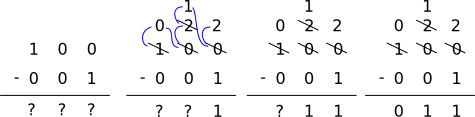
\includegraphics[width=0.5\linewidth]{Figs/entiers_soustraction.pdf}
\end{center}
Dans la soustraction, $100_2 - 001_2$, la première opération $0_2 - 1_2$ nécessite d'emprunter une retenue qui est propagée jusqu'au premier chiffre non nul (jusqu'aux ``centaines''). L'emprunt d'une retenue aux ``centaines'' annule le chiffre des ``centaines'', fait apparaître un deux aux ``dizaines'' (puisque $2^3 = 2.2^2$) auquel on emprunte également une retenue. On finit par faire la soustraction $2 - 1 = 1$. On fait exactement la même chose en base 10, lorsqu'une centaine vaut 10 dizaines et qu'une dizaine vaut 10 unités :
\begin{center}
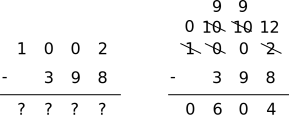
\includegraphics[width=0.5\linewidth]{Figs/entiers_soustraction_base10.pdf}
\end{center}
Comment faire quand la première opérande est plus petite que la deuxième ? Nous allons le voir dans un instant en introduisant des représentations pour les entiers relatifs, dont une particulièrement adaptée pour faire des opérations de soustraction sur les entiers.\\

La multiplication en base $p$ se fait, comme on a appris à l'école, en la posant. En binaire, la multiplication est encore plus simple puisqu'elle repose uniquement sur des décalages et des additions. En effet $11_2 \times 1_2 = 11$, $11_2 \times 10_2 = 110$, ..; Ainsi : $11_2 \times 11_2 = 11_2 \times 1_2 + 11_2 \times 10_2 = 11_2 + 110_2 = 1001_2$ (on retrouve bien $3 \times 3 = 9$). Pour la division, on peut aussi procéder en posant la division en base 2 comme on a appris à la poser en base 10.


%% Attention, l'opération peut générer une retenue résiduelle. Par exemple, avec des représentations binaires sur 3 bits, l'addition 5 + 3 = 8 génère une retenue :\\
%% \begin{center}
%% \begin{tabular}{cccc}
%% & 1 & 0 & 1 \\
%% +&0 & 1 & 1\\
%% \hline
%% (1) &0 &0 &0 
%% \end{tabular}
%% \end{center}


\section{Représentations et opérations avec un nombre fixé de bits}

Jusqu'à maintenant, on ne s'est pas trop soucié du nombre de bits à utiliser pour construire des représentations. Après tout, $10_2 = 2$, $100_2=4$, $1000=8$, ... et on pourrait se dire qu'il suffit d'utiliser un nombre de bits suffisant pour représenter une valeur. Sauf que pour réaliser physiquement un ordinateur, il faut se fixer le nombre de bits qu'on va utiliser. Par exemple, les ordinateurs dits ``32 bits'' et ``64 bits'' utilisent respectivement des représentations des entiers sur 32 et 64 bits. Se fixant un nombre de bits $n$, on ne peut pas représenter plus de $2^n$ valeurs différentes. Le plus petit entier naturel représentable est $0$ et le plus grand entier représentable est $\sum_{i=0}^{n-1} 2^i = 2^n - 1$. Par exemple, sur une machine 32 bits, les entiers naturels sont limités à la plage $[0, 4.294.967.295]$.

\section{Représentation des entiers relatifs}

Le problème de la représentation des entiers négatifs a connu plusieurs réponses au début du développement des ordinateurs. Nous allons notamment voir deux représentations simples (la représentation par offset et la représentation par valeur signée) mais qui ont chacune un inconvénient avant d'introduire la représentation par complément qui s'est imposée. Le problème de la représentation des nombres négatifs consiste à trouver une représentation des entiers relatifs sur $n$ bits qui permettent de réaliser facilement le codage/décodage en base 10 et les opérations arithmétiques.

\subsubsection{Codage par offset}

Le codage par offset (\emph{excess-K}, \emph{offset binary}) est la façon la plus simple de représenter des entiers négatifs et positifs. Il consiste à représenter l'entier le plus négatif par $\overbrace{000\cdots 0}^{k \mbox{ bits}}$ et l'entier le plus positif par $\overbrace{111\cdots 1}^{k\mbox{ bits}}$. Par convention, on représente la plage des entiers $[-2^{k-1}, 2^{k-1}-1]$ (qui contient $2^k$ valeurs). Par exemple, la table ci-dessous donne le codage des entiers par offset pour $k=3$ bits~:
\begin{center}
\begin{tabular}{c|c|c|c|c|c|c|c|c}
Entier $n$ & -4 & -3 & -2& -1 & 0 & 1 & 2 & 3\\
\hline
Codage par offset & $000_{2K}$ & $001_{2K}$ & $010_{2K}$ & $011_{2K}$ & $100_{2K}$ & $101_{2K}$ & $110_{2K}$ & $111_{2K}$
\end{tabular}
\end{center}
Pour coder un entier relatif $n \in [-2^{k-1}, 2^{k-1}-1]$, on commence par lui ajouter $K=2^{k-1}$ et on calcule la représentation non signée de l'entier positif $n+2^{k-1}$. C'est le fait d'ajouter cette constante $K = 2^{k-1}$ qui donne le nom de codage par offset. Remarquez qu'on pourrait choisir une valeur d'offset différente de $2^{k-1}$ pour déplacer arbitrairement, selon les besoins, la plage des entiers représentés. Pour décoder la valeur en base $10$ d'un nombre codé par offset $a_{k-1}a_{k-2}\cdots a_{1}a_{0}$, il suffit de décoder la valeur comme si nous représentions un entier non signé et de soustraire au résultat l'offset K, en d'autres termes~:
\begin{eqnarray*}
 n = \sum_{i=0}^{k-1} a_i 2^i - 2^{k-1}
\end{eqnarray*}
En codage par offset, l'entier $n=0$ est toujours représenté par un $1$ sur le bit de poids fort et des zéros sinon : $0 = 1\overbrace{0\cdots 0}^{k-1\mbox{ bits}}$. On remarquera que les entiers strictement négatif ont un bit de poids fort nul alors que les entiers positifs ont un bit de poids fort égal à 1.

L'addition avec des représentations par offset nécessite un circuit différent de l'addition des représentations non signées. En effet, si nous posons l'addition comme nous l'avons fait avec les représentations non signées, on obtient $(-1)_{2K} + (1)_{2K} = (-4)_{2K}$ :

\begin{center}
\begin{tabular}{ccccc}
  & 0 & 1 & 0 & $011_{2K} = -2$\\
+ & 1 & 0 & 1 & $101_{2K}= 1$\\
\cline{0-3}
  & 1 & 1 & 1 & $111_{2K} = 3$
\end{tabular}
\end{center}

La représentation par offset n'a pas que des inconvénients. Elle a au moins un avantage, les opérations de comparaison sont très simples. Pour savoir si un nombre est plus grand qu'un autre, il suffit de comparer les représentations bit à bit de gauche à droite, c'est à dire le même circuit que pour comparer des représentations non signées\footnote{Un peu plus tard, nous introduisons le codage par complément à deux qui nécessite un circuit différent pour comparer les représentations non signées d'une part et les représentations signées d'autre part}. Dés que deux bits diffèrent, on peut dire quel nombre est plus grand que l'autre :

\begin{algorithm}
\caption{\AlgoName{Comparaison de deux représentations codées par offset} \label{algo:comparaison_offset}}
\begin{algorithmic}[1]
\Function{Comparaison}{$a$, $b$}

\State{$i \gets n-1$}
\While{$a_i == b_i$ et $i \geq 0$}
\State $i \gets i - 1$
\EndWhile
\If{$i < 0$}
\State \Return $a$ égal à $b$
\ElsIf{$a_i = 1$}
\State \Return $a$ plus grand que $b$
\Else
\State \Return $a$ plus petit que $b$
\EndIf
\EndFunction
\end{algorithmic}
\end{algorithm}


%% \begin{algorithm}
%% \caption{\AlgoName{Comparaison de deux représentations codées par offset} \label{algo:comparaison_offset}}
%% \begin{algorithmic}[1]
%% \REQUIRE Deux entiers $a = (a_{n-1}...a_0)_2$, $b=(b_{n-1}...b_0)_2$ codés sur $n$ bits par décalage
%% \STATE{Initialiser $i = n-1$}
%% \WHILE{$a_i == b_i$ et $i \geq 0$}
%% \STATE $i = i - 1$
%% \ENDWHILE
%% \IF{$i < 0$}
%% \RETURN $a$ égal à $b$
%% \ELSIF{$a_i = 1$}
%% \RETURN $a$ plus grand que $b$
%% \ELSE
%% \RETURN $a$ plus petit que $b$
%% \ENDIF
%% \end{algorithmic}
%% \end{algorithm}

\subsubsection{Codage par valeur signée}

Le codage par valeur signée (\emph{sign-magnitude}) consiste à réserver le bit de poids fort pour coder le signe ($a_{k-1} = 0$ pour les entiers positifs et $a_{k-1}=1$ pour les entiers négatifs) et le reste de la représentation $a_{k-2}\cdots a_0$ pour représenter la valeur absolue de l'entier en représentation non signée. L'entier $n=0$ admet alors deux codages $0\overbrace{0\cdots 0}^{k-1\mbox{ bits}}$ (0 positif) ou $1\overbrace{0\cdots 0}^{k-1\mbox{ bits}}$ (0 négatif). Il reste donc un nombre pair de nombres en excluant 0 et un codage sur $k$ bits code donc la plage $[-2^{k-1}+1, 2^{k-1}-1]$. Par exemple, la table ci-dessous donne la codage des entiers par valeur signée pour $k=3$ bits~:

\begin{center}
\begin{tabular}{c|c|c|c|c|c|c|c|c}
Entier $n$ & -3 & -2& -1 & 0 & 1 & 2 & 3 \\
\hline
Codage par valeur signée & $111_{2s}$ & $110_{2s}$ & $101_{2s}$ & $100_{2s}$\mbox{ ou } $000_{2s}$ & $001_{2s}$ & $010_{2s}$ & $011_{2s}$
\end{tabular}
\end{center}

Cette représentation a le désavantage d'avoir deux représentations pour le $0$; Lorsqu'on doit vérifier si un résultat est nul, il faut se comparer à deux représentations possibles. Plus gênant, les opérations arithmétiques nécessitent des circuits différents des opérations arithmétiques sur les représentations non signées. En effet, si on utilise l'addition sur les représentations non signées, le résultat de $1 + (-1)$ est incorrect~:
\begin{eqnarray*}
1 + (-1) = (001)_{2s} + (101)_{2s} = (110)_{2s} = -2
\end{eqnarray*}


%% \subsection{Complément réduit et complément vrai}

%% On va introduire deux notions qui vont nous permettre de définir une représentation astucieuse des entiers négatifs qui facilitera les opérations arithmétiques sur les entiers relatifs\footnote{et se faisant les soustractions sur les entiers positifs}. Ces notions sont les notions de complément réduit et de complément. Le \textbf{complément réduit} d'une représentation en base $p$ $(a_{k-1}...a_0)_p$ est simplement la représentation $(b_{k-1}...b_0)_p$ formée des chiffres $a_i$ complémentés à $p-1$:
%% \begin{eqnarray*}
%% (b_{k-1}...b_0)_p &=&\overline{(a_{k-1}...a_0)_p}\\
%% \forall i, b_i &=& p - 1 - a_i
%% \end{eqnarray*}
%% Nous noterons $(b_{k-1}...b_0)_p = \overline{(a_{k-1}...a_0)_p}$. Par exemple, le complément réduit en base 2 de la représentation $010_2$ est $101_2$ : $\overline{010_2} = 101_2$. Remarquez qu'avec une représentation binaire, il suffit de changer les 0 en 1 et les 1 en 0. \\

%% Lorsqu'un nombre et son complémentaire réduit sont additionnés, on obtient toujours le nombre $(<p-1><p-1>...)_p$. Par exemple $010_2 + \overline{010_2} = 101_2 + 010_2 = 111_2$.\\


%% Nous avons ici utilisé une représentation sur 3 bits, mais nous aurions très bien pu considérer une représentation sur 4 bits ($0010_2$ dont le complément réduit est $1101_2$), sur 5 bits ($00010_2$ dont le complément réduit est $11101_2$), etc...\\

%% Le \textbf{complément} d'une représentation en base $p$ $(a_{k-1}...a_0)_p$ est calculé à partir du complément réduit auquel on ajoute $1$. On notera alors $\overline{(a_{k-1}...a_0)_p}^+ = \overline{(a_{k-1}...a_0)_p} + 1$:
%% \begin{eqnarray*}
%% \overline{(a_{k-1}...a_0)_p}^+ &=& \overline{(a_{k-1}...a_0)_p} + 1\\
%% (b_{k-1}...b_0)_p &=&\overline{(a_{k-1}...a_0)_p}\\
%% \forall i, b_i &=& p - 1 - a_i
%% \end{eqnarray*}

%% \textbf{Pourquoi le complément se comporte comme le négatif du nombre ?}
%% Voir \url{http://www.cs.umd.edu/class/sum2003/cmsc311/Notes/Data/twoscomp.html} pour différentes vues sur le complément à deux qui permet d'expliquer : 1) pourquoi additionner soustraire marche comme additionner des non signés avec la deuxième opérande complémenté, 2) pour complémenter est une involution (fof = id) , ..

%% voir peut être aussi \url{http://igoro.com/archive/why-computers-represent-signed-integers-using-twos-complement/}

\subsection{Complément réduit et complément vrai}

Les deux représentations introduites précédemment (par offset et par valeur signée) ont chacune l'inconvénient de nécessiter des circuits spécialisés (différents de ceux impliqués pour les opérations sur les représentations non signées) pour les opérations arithmétiques. Posons nous donc la question de la représentation des entiers négatifs de la manière suivante : soit une représentation $a_{k-1} ... a_0$ d'un entier $a$ , quelle doit être la représentation $b_{k-1}...b_0$ de la valeur $-a$ de telle sorte que l'addition posée donne $\overbrace{0000}^{k\mbox{ bits}}$ ?\\

\begin{center}
\begin{tabular}{ccccc}
  & $a_{k-1}$ & $a_{k-2}$ & $\cdots$ & $a_0$\\
+ & $b_{k-1}$ & $b_{k-2}$ & $\cdots$ & $b_0$ \\
\hline
  & 0        &  0       &  0       & 0
\end{tabular}
\end{center}

Si on prends $b_i = 1-a_i$ et qu'on ajoute $1$ au résultat , alors :
\begin{center}
\begin{tabular}{ccccc}
  & $a_{k-1}$ & $a_{k-2}$ & $\cdots$ & $a_0$\\
+ & $1-a_{k-1}$ & $1-a_{k-2}$ & $\cdots$ & $1-a_0$ \\
\hline
  & 1        &  1       &  1       & 1\\
+ & 0        & 0        & 0        & 1\\
\hline
(1)& 0     & 0          &0          &0
\end{tabular}
\end{center}
On appelle \textbf{complément à un} de la représentation $a_{k-1}....a_0$, la représentation $(1-a_{k-1})..(1-a_0)$. Le codage par complément à un sur k bits d'un nombre négatif s'obtient en inversant tout les bits (remplacer les 0 par des 1 et les 1 par des 0) de la représentation non signée de sa valeur absolue sur k-1 bits. Par exemple, avec k=3 bits :
\begin{eqnarray*}
3 = 011_2 ; -3 = 100_2
\end{eqnarray*}
On appelle \textbf{complément à deux} de la représentation $a_{k-1}....a_0$, la représentation $(1-a_{k-1})..(1-a_0) + 1$. Le codage par complément à deux s'obtient simplement en inversant tout les bits (pour construire le complément à un) et à ajouter $1$ au résultat. La table ci-dessous donne le codage des entiers par complément pour $k=3$ bits:

\begin{center}
\begin{tabular}{c|c|c|c|c|c|c|c|c|c}
Entier $n$ & -4 & -3 & -2& -1 & 0 & 1 & 2 & 3 \\
\hline
Codage par complément à un & - & 100 & 101 & 110 & 111 ou 000 & 001 & 010 & 011\\
\hline
Codage par complément à deux & 100 & 101 & 110 & 111 & 000 & 001 & 010 & 011
\end{tabular}
\end{center}

Notez que pour la représentation de ``0'', on part de ``000'', on calcule son complément à 1, soit ``111'' auquel on ajoute 1 en gardant le résultat sur 3 bits et donc en ignorant la retenue. Quelques exemples supplémentaires :
\begin{eqnarray*}
42 = 0010\quad1010 \stackrel{\mbox{complément à un}}{\Rightarrow} 1101\quad0101  \stackrel{\mbox{+1}}{\Rightarrow} 1101\quad0110 = -42\\
-42 = 1101\quad0110\stackrel{\mbox{complément à un}}{\Rightarrow} 0010\quad1001  \stackrel{\mbox{+1}}{\Rightarrow} 0010\quad1010 = 42
\end{eqnarray*}

Le ``complément à un'' donne deux représentations du $0$ et permet de représenter la plage des entiers $[-2^{k-1}+1, 2^{k-1}-1]$. La représentation par complément à deux ne donne qu'une représentation du $0$ et permet de représenter les entiers $[-2^{k-1}, 2^{k-1}-1]$. Le bit de poids fort d'un nombre négatif est à 1, le bit de poids fort d'un nombre positif est à 0.\\

On retiendra les étapes de conversion suivante. Pour convertir un entier $n \in [-2^{k-1}, 2^{k-1}-1]$ dans sa représentation en complément à deux :
\begin{itemize}
\item Si $n \geq 0$, on calcule sa représentation non signée
\item Si $n < 0$, on calcule la représentation non signée de $-n$, on inverse tout les bits et on ajoute 1
\end{itemize}
Pour calculer la valeur décimale d'une représentation par complément $a_{k-1}....a_0$ :
\begin{itemize}
\item si $a_{k-1} = 0$, le nombre est positif et sa valeur est $\sum_{i=0}^{k-2} a_i 2^i$,
\item si $a_{k-1} = 1$, le nombre est négatif. Sa valeur absolue est calculée en complémentant la représentation $(1-a_{k-2})..(1-a_0) + 1$ et en calculant sa valeur.
\end{itemize}
On peut aussi directement calculer la valeur décimale d'une représentation par complément à deux grâce à la formule : $(a_{k-1}....a_0)_2 = -a_{k-1}2^{k-1} + \sum_{i=0}^{k-2} a_i 2^i$.


%% Le complément à deux d'un nombre $a = 0a_{k-2}\cdots a_0$ se calcule par~:
%% \begin{eqnarray*}
%% \overbrace{2^{k-1} + \sum_{i=0}^{k-2} (1-a_i)2^i}^{\mbox{complément à un}} + 1 &=& 1 + 2^{k-1} + \sum_{i=0}^{k-2} (1-a_i) 2^i\\
%% &=& 2 + \sum_{i=0}^{k-2} 2^i + \sum_{i=0}^{k-2} (1-a_i) 2^i\\
%% &=& 2 + \sum_{i=0}^{k-2} (2 - a_i) 2^i
%% \end{eqnarray*}


\section{Opérations arithmétiques sur les représentations signées}


\subsection{Additions/Soustractions}
% voir \url{https://en.wikipedia.org/wiki/Method_of_complements} sur comment faire des opérations avec les trois représentations sign-magnitude, one complement, two complement

Nous considérons ici uniquement la représentation par complément à deux, car, comme nous l'avons esquissé précédemment, cette représentation facilite les opérations arithmétiques. L'addition en complément à deux se réalise de la même façon que l'addition sur les représentations non signées :

\begin{tabular}{ccc|cc}
$a$ & $b$ & $r$& Retenue & Reste\\
\hline
0 & 0 & 0 & 0 & 0\\
0 & 1 & 0 & 0 & 1\\
1 & 0 & 0 & 0 & 1\\
1 & 1 & 0 & 1 & 0\\
0 & 0 & 1 & 0 & 1\\
0 & 1 & 1 & 1 & 0\\
1 & 0 & 1 & 1 & 0\\
1 & 1 & 1 & 1 & 1
\end{tabular}

\begin{algorithm}
\caption{\AlgoName{Addition de deux entiers relatifs représentés en complément à deux} \label{algo:addition_binaire_2complement}}
\begin{algorithmic}[1]
\Function{Addition}{$a$, $b$}

\Require Deux entiers $a = (a_{n-1}...a_0)_2$, $b=(b_{n-1}...b_0)_2$ codés sur $n$ bits
\Ensure La représentation $(c_{n-1} ... c_0)_2$ sur \textbf{n bits} de $c = a + b$
\State{$r \gets 0$}
\For{$i=0$ à $n-1$}
\State $c_i \gets \text{reste}(a_i + b_i + r)$
\State $r \gets \text{retenue}(a_i + b_i + r)$
\EndFor
%\State \todo{et la retenue et l'overflow ?}
\State \Return $(c_n c_{n-1} .. c_ 0)$
\EndFunction
\end{algorithmic}
\end{algorithm}



%% \begin{algorithm}
%% \caption{\AlgoName{Addition de deux entiers relatifs représentés en complément à deux} \label{algo:addition_binaire_2complement}}
%% \begin{algorithmic}[1]
%% \REQUIRE Deux entiers $a = (a_{n-1}...a_0)_2$, $b=(b_{n-1}...b_0)_2$ codés sur $n$ bits
%% \ENSURE La représentation $(c_{n-1} ... c_0)_2$ sur \textbf{n bits} de $c = a + b$
%% \STATE{Initialiser $r = 0$}
%% \FOR{$i=0$ \TO $n-1$}
%% \STATE $r = \text{retenue}(a_i + b_i + r)$
%% \STATE $c_i = \text{reste}(a_i + b_i + r)$
%% \ENDFOR
%% \STATE \todo{et la retenue et l'overflow ?}
%% \RETURN $(c_n c_{n-1} .. c_ 0)$
%% \end{algorithmic}
%% \end{algorithm}

Par exemple, pour réaliser l'opération $3 + (-2)$ sur $k=3$ bits, on commencera par construire les représentations par complément à deux de $3$ et $-2$ :
\begin{itemize}
\item[] $3 = (011)_2$
\item[] $2 = (010)_2 \Rightarrow (-2) = (110)_2$
\end{itemize}
et on posera l'addition :

\begin{tabular}{cccc}
& 0 & 1 & 1\\
+& 1 & 1 & 0 \\
\hline
(1) & 0 & 0 & 1
\end{tabular}

La valeur décimale de la représentation en complément à deux $001$ est : $-0\times 2^3 + 1 = 1$. Calculons maintenant $2 + (-3)$ :
\begin{itemize}
\item[] $3 = (011)_2 \Rightarrow (-3) = (101)_2$
\item[] $2 = (010)_2$
\end{itemize}
et on pose l'addition :

\begin{tabular}{cccc}
& 1 & 0 & 1\\
+& 0 & 1 & 0 \\
\hline
(0) & 1 & 1 & 1
\end{tabular}

La valeur décimale de la représentation en complément à deux $111$ est : $-1\times 2^3 + 1 + 2 + 4 = -1$. On trouve également la valeur décimale en complémentant $\overline{111_2} + 001_2= 001_2 = 1$ et en retournant l'opposé.

Utilisant un nombre fixé de bits pour représenter les valeurs, certaines opérations peuvent conduire à des résultats faux. Lorsque le résultat d'une opération arithmétique est plus petit que le plus entier représentable ou plus grand que le plus grand entier représentable, on peut avoir un dépassement de capacité (\textbf{overflow}). Le dépassement de capacité apparaît lorsque l'addtion de deux nombres positifs conduit à la représentation d'un nombre négatif ou lorsque l'addition de deux nombres négatifs conduit à la représentation d'un nombre positif; il ne peut jamais apparaître lors de l'addition d'un nombre positif et d'un nombre négatif. Par exemple, si on additionne $3 + 3$ sur $k=3$ bits, un dépassement de capacité se produit :

\begin{tabular}{cccc}
& 0 & 1 & 1\\
+& 0 & 1 & 1 \\
\hline
(0) & 1 & 1 & 0
\end{tabular}

En effet $110_2$ est la représentation en complément à deux du nombre négatif $-6 \neq 3 + 3$. Le problème apparaît aussi en additionnant des nombres négatifs, $(-3) + (-3)$ sur $k=3$ bits. Les représentations en complément à deux de $-3$ étant $101_2$, l'addition donne:

\begin{tabular}{cccc}
& 1& 0 & 1\\
+& 1 & 0 & 1 \\
\hline
(1) & 0 & 1 & 0
\end{tabular}

La représentation $010_2$ a pour valeur $2 \neq -6$ en complément à deux. Dans le cas précédent, il y a overflow et génération d'une retenue mais il n'y a pas équivalence entre les deux. L'exemple ci-dessous conduit à la génération d'une retenue sans pour autant qu'il y ait dépassement de capacité.
\begin{tabular}{ccccc}
    & 0 & 1 & 1 & $3_2$\\
+   & 1 & 1 & 0 & $(-2)_2$\\
\hline
(1) & 0 & 0 & 1 & $1_2$
\end{tabular}

Une règle que je ne détaillerais pas est qu'il y a dépassement de capacité si et seulement si la retenue entrante lors du calcul du bit le plus à gauche (le bit de signe) est différente de la retenue sortante. Nous ne détaillerons pas plus le débordement de capacité mais c'est un aspect à prendre en compte lorsqu'on réalise des circuits réalisant ces opérations arithmétiques.

%\subsection{Mutliplication/Division}


%\subsection{Généralisation de la méthode des complément en base $p$}



\section{Représentation des nombres réels : virgule fixe et virgule flottante}

\subsection{Représentation par virgule fixe (\emph{fixed-point})}

On va maintenant rapidement présenter des représentations de nombres réels en introduisant la représentation à virgule fixe et la représentation à virgule flottante. Pour comprendre la représentation par virgule fixe, commençons par regarder un exemple en décimal. Le nombre décimal $26.5$ peut se décomposer, en étendant ce que nous avons fait lorsque nous avons introduit la représentations des entiers naturels, de la manière suivante :
\begin{eqnarray*}
26.5 = 2 \times 10^1 + 6 \times 10^0 + 5 \times 10^{-1}
\end{eqnarray*}
Si on utilise maintenant une représentation binaire, on peut affecter à chacune des positions une puissance de $2$ : $2^2, 2^1, 2^0, 2^{-1}, 2^{-2}, ...$. Le seul problème est de savoir o{\`u} placer la virgule lorsqu'on voit la représentation $110101$. Si la virgule se trouve à la fin du mot, alors $110101_2 = 2^0 + 2^2 + 2^4 + 2^5 = 53$. Si la virgule se trouve juste avant la fin du mot, disons $11010.1$, alors : $11010.1 = 2^{-1} + 2^1 + 2^3 + 2^4 = 26.5$. Il n'y a pas d'autre choix que de se fixer une convention en précisant le nombre de bits $n_e$ utilisés pour représenter la partie entière et le nombre de bits $n_f$ utilisés pour représenter la partie fractionaire. Une représentation à virgule fixe avec $n_e$ bits pour la partie entière et $n_f$ bits pour la partie fractionaire sera notée $Q<n_e>.<n_f>$. Par exemple, $Q2.14$ utilise $2$ bit pour la partie entière et $14$ bits pour la partie fractionnaire avec une représentation sur $16$ bits en tout.

Pour construire la représentation à virgule fixe du nombre réel $26.5$, on isolera la partie entière $26$ et la partie fractionnaire $.5$ La partie entière s'écrit $26 = 16 + 8 + 2 = (11010)_2$ et la partie fractionnaire $0.5 = 2^{-1}$. Avec une représentation à virgule fixe $Q7.1$, le réel $26.5$ s'écrit $00110101$. On peut remarquer que certaines opérations s'effectuent très simplement avec une représentation par virgule fixe. Par exemple, multiplier par 2 la représentation $00110101$ revient à décaler la représentation à gauche et à construire sur $8$ bits la représentation $01101010$ dont la valeur\footnote{la formule pour calculer la valeur s'applique ici parce que la valeur en positive. Si des nombres négatifs sont représentés, comme décrit un peu plus loin, il faudra faire attention au bit de signe}, dans une représentation $Q7.1$ est :
\begin{eqnarray*}
\sum_{i=0}^{k-1} a_i 2^{i-n_f} &=& 0\times 2^{-1} + 1 \times 2^0 + 0 \times 2^1 + 1 \times 2^2 + 0 \times 2^3 + 1 \times 2^4 + 1 \times 2^5 + 0 \times 2^6\\
 &=& 1 + 4 + 16 + 32 = 53
\end{eqnarray*}

Remarquez que pour calculer la valeur décimale d'une représentation $Q<n_e><n_f>$, il suffit d'interpréter la représentation comme une représentation d'un entier naturel et de multiplier la valeur décimale trouvée par $2^{-n_f}$ puisque :
\begin{eqnarray*}
\sum_{i=0}^{k-1} a_i 2^{i-n_f} = 2^{-n_f} \sum_{i=0}^{k-1} a_i 2^{i}
\end{eqnarray*}
Et on retrouve à droite de l'équation le terme $\sum_{i=0}^{k-1} a_i 2^{i}$ pour calculer la valeur décimale d'un \textbf{entier naturel}.

Comme pour la représentation des entiers négatifs utilisait le complément à deux, la représentation des nombres négatifs en virgule fixe utilise également le complément à deux. Par exemple, en notation à virgule fixe $Q4.2$, le réel $3.5$ s'écrit : $3.5 = 2^1 + 2^0 + 2^{-1} = 001110_2$. Son complément à deux est $-3.5 = 110010_2$. On peut alors calculer $5.25 - 3.5$ :

\begin{tabular}{cccccccr}
& 0 & 1 & 0 & 1 & 0 & 1 & (5.25)\\
+ & 1 & 1 & 0 & 0 & 1 & 0 & (-3.5)\\
\hline
(1) & 0& 0& 0& 1 & 1 & 1 & (1.75)
\end{tabular}

Et dans le sens inverse, en notant que $-5.25 = 101011_2$:

\begin{tabular}{cccccccr}
& 1 & 0 & 1 & 0 & 1 & 1 & (-5.25)\\
+ & 0 & 0 & 1 & 1 & 1 & 0 & (3.5)\\
\hline
(0) & 1& 1& 1& 0 & 0 & 1 & (-1.75)
\end{tabular}

Comme le bit de poids fort de $111001_2$ est égal à un, le nombre est négatif, son opposé est représenté par le complément à deux de $\overline{111001_2} + 1_2 = 000111_2$ dont la valeur avec la représentation Q4.2 est bien $1\times 2^0 + 1 \times 2^{-1} + 1 \times 2^{-2} = 1.75$. Pour calculer directement la valeur décimale $a$ d'une représentation signée à virgule fixe $a_{k-1}...a_0$ dans un système $Q<n_e><n_f>$, il faut utiliser une formule similaire au calcul de la valeur d'un entier d'une représentation en complément à deux :
\begin{eqnarray*}
a_{10} = 2^{-n_f} (-a_{k-1} 2^{k-1} + \sum_{i=0}^{k-2} a_i 2^i), k = n_e + n_f
\end{eqnarray*}
La valeur signée de $111001_2$ est $-7$, donc la valeur de $111001_2$ dans le système $Q4.2$ est $2^{-2} \times (-7) = -1.75$.

Pour finir, remarquez que les opérations arithmétiques sur les représentations à virgule fixe sont identiques aux opérations arithmétiques sur les entiers, contrairement aux opérations arithmétiques sur les représentations à virgule flottante que nous allons voir dans un instant. Cela conduit parfois à préférer cette représentation dans des applications de traitement du signal.


\subsection{Représentation par virgule flottante (\emph{floating-point})}

Dans les années 1980-1990, le standard IEEE-754 a été introduit pour représenter les nombres réels avec une représentation dite à virgule flottante. Une version mise à jour a été proposée en 2008 \citep{IEEE754}. Le standard a été mis au point pour apporter un certain nombre de garanties quand aux erreurs introduites par le fait qu'on travaille en précision finie. Ce standard permet également de représenter l'ensemble étendu des réels auquel est ajouté des nombres spéciaux qNan et sNan : $S = \mathbb{R} \cup \{-\infty, \infty\} \cup \{\mbox{sNan}, \mbox{qNan}\}$. Les ``nombres'' sNan et qNan permettent de gérer des exceptions en représentant les résultats d'opérations telles que 0/0, $\infty/\infty$, $\sqrt{x}, x < 0$, ... .

La représentation par virgule flottante est basée sur la notation scientifique des nombres. La notation scientifique d'un nombre décimal est de la forme :
\begin{eqnarray*}
\mbox{En base 10} : x = \pm m \times 10^{e}, m \in [0, 10[, e \in \mathbb{Z} 
\end{eqnarray*}
Dans cette notation, $m$ est appelé la mantisse, et $e$ l'exposant. Il existe des valeurs pour lesquelles plusieurs représentations sont possibles dans cette notation. Par exemple, $1245 = 1.245 \times 10^3 = 0.1245 \times 10^4 = 0.01245 \times 10^5$. Dans le standard IEEE, les représentations $0.1245 \times 10^4$, $0.01245 \times 10^5$, ..., i.e. telles que $m \in [0, 1[$, sont appelées \textbf{les représentations dénormalisées} de la valeur $1245$. La représentation $1.245 \times 10^3$, i.e. telle que $m \in [1, 10[$, est appelée \textbf{la représentation normalisée} de la valeur $1245$. La chose importante à noter ici est qu'\textbf{il peut exister plusieurs représentations dénormalisées mais une unique représentation normalisée}\footnote{Cela veut notamment dire que pour comparer deux nombres en virgule flottante, il faudra s'assurer de normaliser les représentations et ne pas faire une comparaison bit à bit naïvement}. Un nombre fixé de bits étant utilisé pour représenter la mantisse ($m=1.245$, $m=0.1245$, $m=0.01245$), la représentation normalisée est celle qui utilise au mieux l'espace de représentation puisque les représentations dénormalisées occupent de l'espace inutilement pour représenter les $0$ en tête du nombre. Néanmoins, ces représentations dénormalisées permettent d'accroître le domaine représentable puisque $e$ est borné. Prenons un exemple, si l'exposant $e \in [-128, 127]$ et supposons qu'on s'autorise $3$ chiffres pour représenter la mantisse. Si nous considérons uniquement des représentations normalisées, le plus petit nombre positif non nul représentable est $1.00 \times 10^{-128}$. En autorisant des représentations dénormalisées, le plus petit nombre positif non nul représentable est $0.01 \times 10^{-128}$.


En généralisant à n'importe quelle base $p$, la notation scientifique s'écrit :
\begin{eqnarray*}
\mbox{En base p} : x = \pm m \times p^{e}, m \in [0, p[, e \in \mathbb{Z} 
\end{eqnarray*}
et en binaire, on a la propriété intéressante que la mantisse est toujours comprise dans l'intervalle $[0, 2[$, i.e. le bit de poids fort de la mantisse est $0$ ou $1$ :
\begin{eqnarray*}
\mbox{En base 2} : x = \pm m \times 2^{e}, m \in [0, 2[, e \in \mathbb{Z} 
\end{eqnarray*}

Pour représenter un nombre réel sous la forme d'une séquence de bits, il faut représenter :
\begin{itemize}
\item le signe : 1 bit suffit
\item la mantisse sur $n_m$ bits
\item l'exposant sur $n_e$ bits
\end{itemize}
pour un total de $k = 1 + n_m + n_e$ bits. Le standard IEEE-754 introduit plusieurs standards $binary-k$ en précisant la taille des mots pour représenter la mantisse et l'exposant, en voici quelques un~:
\begin{itemize}
\item binary-16 : $k=16$ bits, 1 bit de signe, $n_e = 5$ bits pour l'exposant, $n_m=10$ bits pour la mantisse
\item binary-32 : $k=32$ bits, 1 bit de signe, $n_e = 8$ bits pour l'exposant, $n_m=23$ bits pour la mantisse
\item binary-64 : $k=64$ bits, 1 bit de signe, $n_e = 11$ bits pour l'exposant, $n_m=52$ bits pour la mantisse
\end{itemize}
Schématiquement, une représentation à virgule flottante se présente comme ci-dessous :

\begin{center}\begin{tabular}{|c|c|c|}
\hline
signe S (1 bit)& exposant E ($n_e$ bits)& mantisse M ($n_m$ bits)\\
\hline
\end{tabular}
\end{center}
La valeur $v$ de cette représentation s'obtient alors comme suit :
\begin{itemize}
\item Si $E = 11\cdots 1_2 = 2^{n_e} - 1$ et $M = 00\cdots 0_2 = 0$, alors $v = (-1)^S \infty$,
\item Si $E= 11\cdots 1_2 = 2^{n_e} - 1$ et $M \neq 0$, alors $v \in \{\mbox{qNan}, \mbox{sNan}\}$,
\item Si $E = 00\cdots 0_2 = 0$ et $M = 00\cdots 0_2 = 0$, alors $v = (-1)^S 0$, i.e. ($\pm 0$),
\item Si $E = 00\cdots 0_2 = 0$ et $M \neq 0$, alors nous avons une représentation dénormalisée et 
$$v = (-1)^S . 2^{1-K} M . 2^{-m_n}$$ avec $K = 2^{n_e-1}-1$,
\item Si $E \in [1, 2^{n_e} - 2]$, alors nous avons une représentation normalisée et 
$$v = (-1)^S . 2^{E - K} (1 + M . 2^{-m_n})$$
avec $K = 2^{n_e-1}-1$
\end{itemize}

\subsection{Exemple de la représentation en virgule flottante binary-16}

Dans cette partie, on se propose de regarder un peu plus en détails les valeurs représentées par un standard particulier, le standard binary-16, pour le codage des réels en virgule flottante. On donne dans la table ci-dessous quelques examples de représentations binaires binary-16 ainsi que la valeur représentée. Pour rappel, dans le standard binary-16, on utilise une représentation sur 16 bits avec $1$ bit de signe, $n_e=5$ bits pour l'exposant, $n_m=10$ bits pour la mantisse. Pour le codage de l'exposant, l'excès est $K = 15$. L'exposant peut donc prendre des valeurs dans $[-14, 15]$

\begin{center}\begin{table}[htbp]
\begin{tabular}{ccc|c|c}
\multicolumn{3}{c}{Représentation binary-16} & Valeur représentée & Note\\
Signe & Exposant & Mantisse & & \\
\hline\hline
0&00000&0$\cdots$0 & +0 & \\
1&00000&0$\cdots$0 & -0 & \\
s&00000&0$\cdots$01 & $(-1)^s 2^{-14} 1.2^{-10} = (-1)^s 2^{-24}$ & Plus petit réél dénormalisé\\
s&00000&0$\cdots$10 & $(-1)^s 2^{-14} 2.2^{-10} = (-1)^s 2^{-23}$ & Second plus petit réel\\
s&00000&1$\cdots$11 & $(-1)^s (2^{-14} - 2^{-24})$ & Plus grand réel dénormalisé\\
s&00001&0$\cdots$00 & $(-1)^s 2^{1-15} = (-1)^s 2^{-14}$ & Plus petit réel normalisé \\
s&11110&1$\cdots$11 & $(-1)^s 2^{15} (2 - 2^{-10})$& Plus grand réel normalisé \\
s&11111&0$\cdots$00 & $(-1)^s \infty$ & \\
x&11111& M, $M \neq 0$ & NaN (sNan ou qNan) & Exception, e.g 0/0, ..
\end{tabular}
\caption{Quelques exemples de représentation binaire du standard binary-16 de la norme IEEE-754 et de la valeur représentée. Dans les représentations binaires, le chiffre "x" indique 0 ou 1 indifféremment, i.e. signifie que la valeur de ce chiffre n'est pas pris en compte.}
\end{table}
\end{center}

Pour donner un ordre de grandeur en base 10~: $2^{-24} \approx 6.10^{-8}$, $2^{15} (2-2^{-10}) = 65504$.
%% A priori on utilise le excess K pour la représentation de l'exposant.

%% On a vu jusqu'à maintenant comment représenter des nombres entiers naturels et relatifs. On aimerait aussi pouvoir représenter en binaire des nombres réels. 
%% \begin{itemize}
%% \item artihmétique à virgule fixe : von Neumann dans les années 1950
%% \item arithmétique à virgule flotante : introduite par Zuse dans les années 1940, 1950
%% \item a priori on ne maitrise pas bien les arrondis avec les floating points contrairement au fixed point. Certains logiciels utilisent plutôt le fixed point pour cette raison
%% \item \url{http://www.cs.umd.edu/class/sum2003/cmsc311/Notes/Data/float.html} : présente la norme IEEE-754 ; aussi une raison de l'exposant en excess -K : il dit que les comparaisons sont plus simples que si on utilisait du complément à deux. mais donc j'imagine aussi que ça ne gène pas pour d'autres opérations sur les exposants... en gros comment gères t'on les opérations sur ces floatants ?
%% \end{itemize}




\section{Représentation des caractères}

En informatique, une information est codée exclusivement par des séquences de 0 et 1. On a vu précédemment comment coder des entiers et des réels en binaire mais on a également besoin de trouver un moyen de coder du texte (caractères '0', '1', 'A', 'é'; ponctuation ! , ? espace, .. ; symboles spéciaux comme \euro, \$, @) comme une séquence de 0 et 1. Pour coder/décoder des caractères, il faut se mettre d'accord sur le nombre de bits utilisés pour représenter un caractère (pour pouvoir ségmenter une longue séquence de 0 et de 1 en caractères) et sur une table associant un mot binaire à un caractère. Dans les années 1980-1990, il y avait plusieurs normes pour coder les caractères qui sont apparues à travers le monde: l'ASCII aux Etat-unis, le KOI8-R en Russie, ... Ces normes proposaient d'encoder les caractères sur 7 ou 8 bits mais le fait que les normes soient nées indépendemment les unes des autres rendait les systèmes difficilement interopérables et très spécifiques (en Russe, il faut pouvoir représenter l'alphabet cyrillique). Par exemple, l'ASCII (American Standard Code for Information Interchange) développé aux Etat-Unis, utilise 7 bits (128 valeurs possibles) pour coder des caractères dont les codes apparaissent sur la table suivante\footnote{La table ASCII est produite par Victor Eijkhout}. 

\input{ascii.tex}

Vous l'aurez remarqué, il nous manque nos caractères accentués; en effet, les américains n'utilisent pas de caractères accentués; et bien sûr bien d'autres caractères manquent pour satisfaire toutes les langues. Il y a eu donc une flopée de normes dont notamment les normes ISO-8859-x, avec x variant de 1 à 16, chacune encodant des caractères d'une langue différente, sur 8 bits. Par exemple, la norme ISO 8859-1 couvre les caractères de la plupart des langues européennes, la norme ISO 8859-5 couvre l'alphabet cyrillique, ... Les normes ISO étendent la norme ASCII en utilisant les mêmes 128 premiers caractères. Comme la norme ISO propose un encodage sur 8 bits, il y a 128 caractères supplémentaires à utiliser. En pratique ces 128 caractères supplémentaires ne sont pas tous utilisés mais en tout cas, en fonction de la norme considérée, ils ne représentent pas la même valeur; Quelques caractères des différentes normes ISO-8859-x sont représentés sur la figure \ref{fig:iso8859}.

\begin{figure}[htbp]
\begin{center}
\includegraphics[width=0.5\columnwidth]{Figs/iso8859.png}
\end{center}
\caption{\label{fig:iso8859}Extrait des normes ISO-8859-x disponibles. Source: \protect\url{https://fr.wikipedia.org/wiki/ISO_8859}.}
\end{figure}

Plus récemment, un nouveau format, issu du standard Unicode et de la norme ISO 10646, commence à s'imposer : le format UTF-8. Ce format code tout les caractères possibles en utilisant un nombre variable de mots de 8 bits (le format UTF-8 accepte jusqu'à 4 octets). 


\section{Un exemple}

Pour terminer cette partie, j'aimerais revenir sur la différence entre une valeur et son représentant. Si on considère la séquence binaire ci-dessous (représentée en hexadécimal pour rester compact):
\begin{center}
$(626F6E6A6F757221)_{16}$
\end{center}
elle peut représenter plusieurs valeurs :
\begin{itemize}
\item la chaîne de caractères ``bonjour!'' si je considère que la séquence représente des caractères codés en ASCII
\item la valeur 7 093 009 341 547 377 185 si je considère que la séquence représente un entier codé sur 64 bits
\item l'image \includegraphics[width=0.3\linewidth]{Figs/code_img.pdf} si je considère que chaque bloc de 8 bits code le niveau de gris d'un pixel considéré comme noir pour 0 et blanc pour 255,
\item ....
\end{itemize}

%% import numpy as np
%% import matplotlib.pyplot as plt
%% z = np.array([int(ord(c)) for c in 'bonjour!'])
%% z = z.reshape((1,8))
%% plt.figure(facecolor='white')
%% plt.imshow(z, interpolation='None', cmap='gray')
%% plt.axis('off')
%% plt.savefig("code_img.pdf",bbox_inches='tight')
%% plt.show()


%% \section{Codage minimal et codage robuste}

%% \subsection{Codage minimal}

%% Jusqu'à maintenant, nous avons imposé aux représentations d'avoir une taille fixe et nous verrons plus tard que cela facilite la réalisation matérielle d'une machine manipulant ces représentations. Mais, si la question était posée sous la forme ``quel codage utiliser pour représenter un message avec le plus petit nombre de bits ?'', la réponse serait un peu différente de ce que nous avons présenté précédemment. Une réponse est fournie dans le cadre de la théorie de l'information introduite par Shannon dans les années 1940-1950. Ce serait bien trop ambitieux pour ce cours que de présenter ce sujet. 

%% La figure \ref{fig:distribution_francais} représente la distribution des lettres dans un corpus d'un peu plus d'un million de documents en Français. On y voit clairement que la lettre ``e'' est sur-représentée. L'idée derrière un codage de taille variable est d'utiliser une séquence binaire de taille $n_c$ pour représenter le caractère ``c'' de telle sorte que $n_c$ décroit quand la fréquence d'apparition $f_c$ du caractère ``c'' augmente.

%% \begin{figure}
%% 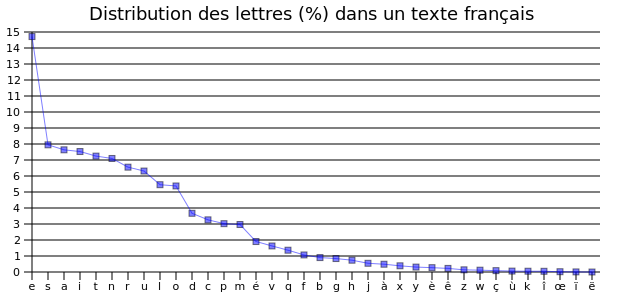
\includegraphics[width=0.75\linewidth]{Figs/frequence_lettres_francais.svg}
%% \caption{\label{fig:distribution_francais}Distribution des lettres calculés à partir d'un corpus de plus d'un million de lettres.}
%% \end{figure}

%% On pourra par exemple utiliser un codage de la forme :
%% \begin{tabular}{cc}
%% Caractère & Représentation \\
%% e & 0\\
%% s & 10\\
%% a & 110\\
%% i & 1110\\
%% ... & ...
%% \end{tabular}

%% \subsection{Codage robuste}

%% Supposons maintenant que le critère pour trouver un codage pour un message soit sa robustesse .... 



%%%%% Elements de circuits logiques

\chapter{La couche physique et la couche logique}

Nous venons de voir comment coder des informations en binaire. Nous allons ici nous intéresser à la manière de manipuler ces représentations et notamment proposer des algorithmes permettant d'effectuer des opérations arithmétiques sur les représentations binaires des nombres. Pour le moment, on ne sait faire ces opérations que sur le papier mais, pour automatiser des calculs, il faut mettre au point des mécanismes physiques (mécaniques, électroniques, optiques) réalisant ces opérations. On commencera par introduire le transistor qui est l'élément majeur des circuits électroniques que nous allons présenter\footnote{Un microprocesseur des années 1970 comptait quelques milliers de transistor. En 2015, les microprocesseurs multi-coeurs contiennent une dizaine de milliards de transistors ($10.10^{9}$). Source : \protect\url{https://en.wikipedia.org/wiki/Transistor_count}} et très vite, nous en ferons l'abstraction en introduisant les portes logiques à partir desquelles nous élaborerons différents circuits particuliers qui nous permettrons de construire notre première architecture.

\section{Un peu d'électronique}

Avant de voir plus en détails comment se construit un ordinateur, il faut introduire quelques éléments d'électronique pour comprendre comment représenter physiquement un bit ainsi que des circuits électroniques permettant de manipuler ces signaux. Ces circuits vont principalement reposer sur le transistor et nous allons voir pourquoi ce composant est particulièrement bien adapté. 

%Attention, les circuits électroniques présentés dans les sections suivantes sont à considérer comme des \textbf{circuits de principe}. Bien qu'il soient valables, ils ne sont pas utilisés en pratique pour réaliser les fonctions qu'on va présenter pour diverses raisons de performances. Je vous suggère de vous diriger vers un véritable cours d'électronique pour en savoir plus à ce sujet.

\subsection{Niveaux logiques et valeurs de tension}

La représentation d'un bit se fait en électronique par des niveaux de tension. Disons\footnote{Les circuits logiques utilisent généralement des tensions entre 0V et 3.3V ou entre 0V et 5V. On utilise ici 1V à titre d'illustration.}, par exemple, $0$V pour un bit au niveau bas $b=0$ et $1$V pour un bit au niveau haut $b=1$. Cela étant dit, quel est l'état binaire d'une tension à $0.75$ V? probablement $b=1$; $0.25$ V ? probablement $b=0$ et qu'en est-il de $0.49$V et $0.51$V ? A cause des défauts de fabrication, des perturbations possibles de l'environnement du circuit, il est nécessaire d'introduire des tolérances et de définir des domaines de tension acceptable pour définir chacun des niveaux logiques. Les circuits électroniques que nous allons considérer vont transformer des tensions d'entrées $V_{in}$ en des tensions de sortie $V_{out}$ (fig. \ref{fig:VTC}a) et la fonction reliant les deux est appelée \textbf{fonction caractéristique de transfert} (\emph{Voltage Transfer Characteristics}).

\begin{figure}[htbp]
\centering\begin{tabular}{cc}
\includegraphics[width=0.5\linewidth]{Figs/vtc.pdf}& 
\includegraphics[width=0.5\linewidth]{Figs/VTC_connect.pdf}\\
a) & b)
\end{tabular}
\caption{\label{fig:VTC} a) Vision schématique d'un circuit transformant une tension $V_{in}$ en une tension $V_{out}$. La fonction reliant les deux est la fonction caractéristique de transfert. b) Des marges de bruit doivent être introduites pour garantir le bon fonctionnement de composants interconnectés. }
\end{figure}

Les fabricants définissent des domaines pour les entrées et sorties dans lesquels ils garantissent le fonctionnement de leur circuit :
\begin{itemize}
\item pour les entrées :
\begin{itemize}
\item $v_{il}$ : tension maximale d'entrée pour que le composant la considère à l'état bas $b_{in} = 0$
\item $v_{ih}$ : tension minimale d'entrée pour que le composant la considère à l'état haut $b_{in} = 1$
\end{itemize}
\item pour les sorties :
\begin{itemize}
\item $v_{ol}$ : tension maximale de sortie que le composant produit pour une sortie à l'état bas $b_{out} = 0$
\item $v_{oh}$ : tension minimale de sortie que le composant produit pour une sortie à l'état haut $b_{out} = 1$
\end{itemize}
\end{itemize}

%\todo{Quelques exemples de valeur vil, vol, ... à partir des liens en commentaire dans le latex}.\\


Quelle que soit la fonction réalisée par le circuit, le fabricant garantie que si l'entrée représente un état binaire valide ($V_{in} \in [0, v_{il}] \cup [v_{ih}, V_{cc}]$), alors la sortie représentera un état binaire valide ($V_{out} \in [0, v_{ol}] \cup [v_{oh}, V_{cc}]$). Par ailleurs, pour prendre en compte les imperfections de son circuit, les tolérances de sortie sont plus strictes que les tolérances d'entrée : une sortie est considérée à l'état haut si $v_{out} \geq v_{oh} > v_{ih}$ et à l'état bas si $v_{out} \leq v_{ol} < v_{il}$. En effet, considérons que nous interconnections deux composants comme sur la figure~\ref{fig:VTC}b. Différentes sources de bruit dûes à l'environnement du circuit conduisent au fait que le potentiel de sortie $V_{oA}$ est différent du potentiel d'entrée $V_{iB}$. Le potentiel de sortie $V_{oA}$ ne doit pas être vu comme un potentiel constant mais comment étant perturbé par un certain bruit. Si on définit $v_{ol} = v_{il}$, et que $V_{oA} = v_{ol}$, i.e. la tension maximale pour indiquer un niveau logique bas en sortie de A, la perturbation peut conduire à ce que ce niveau bas soit considéré comme invalide pour le composant B. C'est donc pour garantir qu'une sortie valide demeure une entrée valide, malgré le bruit de transimission, qu'on impose à ce que $v_{ol} < v_{il}$ et $v_{oh} > v_{ih}$. Les différences $v_{il} - v_{ol}$ et $v_{oh} - v_{ih}$ sont appelées \emph{marges de bruit}. Il y aurait beaucoup d'autres choses à dire sur la compatibilité des circuits interconnectés mais nous nous arrêterons là dans ce cours et je vous renvois vers un cours d'électronique pour en savoir plus. 

%\begin{figure}[htbp]
%\centering\includegraphics[width=0.5\linewidth]{Figs/VTC_connect.pdf}
%\caption{\label{fig:VTC_connect} Des marges de bruit doivent être introduites pour garantir le bon fonctionnement de composants interconnectés.}
%\end{figure}

\begin{figure}[htbp]
\centering\includegraphics[width=0.5\linewidth]{Figs/vtc_forbidden_labels.pdf}\includegraphics[width=0.5\linewidth]{Figs/vtc_forbidden.pdf}
\caption{\label{fig:VTC_forbidden} Les domaines interdits pour la fonction caractéristique de transfert sont représentés en rouge. Quelle que soit la fonction réalisée par le circuit, la fonction caractéristique de transfert devra toujours éviter les domaines interdits pour s'assurer qu'une entrée valide donne toujours une sortie valide. La fonction représentée en noir est une fonction valide.}
\end{figure}

Pour en revenir à un seul composant, notez que rien n'interdit de produire une sortie valide si l'entrée est invalide. Cela conduit ainsi à définir des domaines interdits pour la fonction caractéristique de transfert comme illustré sur la figure \ref{fig:VTC_forbidden}, domaines dans lesquels il est interdit de faire passer la fonction de transfert caractéristique.

Raisonner avec la fonction caractéristique de transfert permet d'identifier une caractéristique des circuits permettant de manipuler des ``représentations binaires'' : ce circuit doit utiliser des composants non linéaires. Au début de l'informatique, dans les années 1930-1940, on utilisait des relais électromécaniques comme par exemple le relais de Joseph Henry illustré sur la figure~\ref{fig:relay}.

\begin{figure}[htbp]
\centering\includegraphics[width=0.5\linewidth]{eps/relay.jpg}
\caption{\label{fig:relay} Relai électromécanique de Joseph Henry. Branchons $v_{out}$ sur la patte 1, $v_{cc}$ sur la patte 4, la masse sur la patte 5 et $v_{in}$ sur la bobine, on obtient alors un inverseur. Si $v_{in}=0$, la languette métallique 10 relie la patte 1 à la patte 4 donc $v_{out}=v_{cc}$. Si $v_{in} = v_{cc}$, le champ magnétique de la bobine conduit à placer la languette métallique 10 en contact avec la pièce 12 et donc $v_{out}=0$. Illustration de \url{http://history-computer.com}.}
\end{figure}

En pratique, les relais sont encombrants, sujets aux interférences, peu robustes dans le temps puisque mécaniques, gourmands en énergie, ... Dans les années 1950 est apparu le transistor, un interrupteur électronique commandable qui a révolutionné l'informatique.

\subsection{Transistors CMOS et inverseur}

Comme nous venons de le voir, il nous faut disposer d'un composant électronique dont la fonction caractéristique de transfert est non linéaire. Le transistor, apparu dans les années 1950 est justement un composant non linéaire. Il existe plusieurs technologies pour réaliser des transistors (TTL, MOS, ..) et ce n'est pas le sujet de ce cours que de les présenter. On ne s'intéressera qu'à une technologie : le transistor MOSFET (Metal Oxyde Field Effect Transistor) et on va s'abstraire du transistor en le voyant comme un interrupteur commandable. Des transistors TTL et MOS sont représentés sur la figure \ref{fig:transistor_bipolaire} et les transistors MOS sont ceux représentés sur les figures \ref{fig:transistor_bipolaire}c, d. Je vous renvois vers un cours de physique des semi-conducteurs pour comprendre le fonctionnement de ces transistors. Nous retiendrons ici deux états de fonctionnement du transitor (passant/saturé ou bloqué) et que l'état dans lequel se trouve le transistor dépends de la différence de potentiel entre la grille et la source.

\begin{figure}
\begin{center}
\begin{tabular}{cccc}
\begin{circuitikz}
\draw	(0,0) node[npn](npn1){};
\node at ($(npn1.B) - (0.5,0)$) {Base};
\node at ($(npn1.E) - (0, 0.5)$) {Emetteur};
\node at ($(npn1.C) + (0, 0.5)$) {Collecteur};
\end{circuitikz} &
\begin{circuitikz}
\draw	(0,0) node[pnp](pnp1){};
\node at ($(pnp1.B) - (0.5,0)$) {Base};
\node at ($(pnp1.E) + (0, 0.5)$) {Emetteur};
\node at ($(pnp1.C) - (0, 0.5)$) {Collecteur};
\end{circuitikz} &
\begin{circuitikz}
\draw (0, 0) node[nmos] (nmos1) {};
\node at ($(nmos1.gate) - (0.5,0)$) {Grille};
\node at ($(nmos1.drain) + (0, 0.5)$) {Drain};
\node at ($(nmos1.source) - (0, 0.5)$) {Source};
\end{circuitikz} &
\begin{circuitikz}
\draw (0, 0) node[pmos] (pmos1) {};
\node at ($(pmos1.gate) - (0.5,0)$) {Grille};
\node at ($(pmos1.drain) - (0, 0.5)$) {Drain};
\node at ($(pmos1.source) + (0, 0.5)$) {Source};
\end{circuitikz} \\
a) & b) & c) & d)
\end{tabular}
\end{center}
\caption{\label{fig:transistor_bipolaire} a) Transistor bipolaire NPN. b) Transistor bipilaire PNP. c) Transistor unipolaire NMOS. d) Transistor unipolaire PMOS}
\end{figure}

Pour ce qui nous concerne dans ce cours, un transistor est abstrait comme un interrupteur commandable (fig. \ref{fig:circuits_mos}a):
\begin{itemize} 
\item Pour un transistor NMOS : si \textbf{une tension nulle est appliquée à la grille}, aucun courant ne circule entre le drain et la source : \textbf{le transistor est bloqué}. Si \textbf{une tension positive est appliquée à la grille}, un courant peut circuler entre le drain et la source : \textbf{le transistor est passant}.
\item Pour un transistor PMOS : si \textbf{une tension nulle est appliquée à la grille}, un courant peut circuler entre la source et le drain : \textbf{le transistor est passant}. Si \textbf{une tension positive est appliquée à la grille}, aucun courant ne circule entre la source et le drain : \textbf{le transistor est bloqué}.
\end{itemize}
La technologie CMOS (Complementary Metal Oxyde Semi Conductor) utilise des transistors en paire PMOS et NMOS placés de manière symétrique (fig. \ref{fig:circuits_mos}b) :
\begin{itemize}
\item les PMOS sont disposés entre l'alimentation $V_{cc}$ et la sortie du circuit; on parle de réseau ``pull-up''
\item les NMOS sont disposés entre la sortie et la masse; on parle de réseau ``pull-down''
\end{itemize}

\begin{figure}[htbp]
   \begin{minipage}[c]{.56\linewidth}
\includegraphics[width=\columnwidth]{Figs/nmospmos.pdf} \\\centering a)
   \end{minipage} \hfill
   \begin{minipage}[c]{.25\linewidth}
\includegraphics[width=\columnwidth]{Figs/circuits_mos.pdf}\\\centering b)
   \end{minipage}
\caption{\label{fig:circuits_mos} a) Les transistors NMOS et PMOS peuvent être vus comme des interrupteurs commandables dont l'état dépends de la différence de potentiel entre la source et la grille. Fixant le potentiel de la source à $V_{cc}$ pour le PMOS et à la masse pour le NMOS, le transitor est commandé par le potentiel appliqué à la grille. b) En technologie CMOS, les circuits à base de transistor MOS sont construits en utilisant des paires de transistors de type P et de type N. Les types P relient toujours l'alimentation à la sortie et les types N la sortie à la masse.}
\end{figure}

Un transistor est un système physique auquel il faut un certain temps pour passer entre les états passant et bloqué. Un transistor unipolaire CMOS mets quelques picosecondes ($10^{-12}s$) pour commuter. En pratique, le transistor se trouve dans un circuit : soit un circuit de mesure, soit interconnecté avec d'autres composants. Il faut alors prendre en compte une capacité parasite de sortie et le temps de commutation est dépendant de cette capacité et des résistances internes du transistor et qui conduisent à des temps de commutation de l'ordre de la nanoseconde.

\begin{figure}[htbp]
   \begin{minipage}[c]{.46\linewidth}
\begin{circuitikz}[scale=0.7, every node/.style={scale=0.7}]
\draw[color=black, thick]
        (0,1.0) node[nmos](nmos1){}
        (0,3.0) node[pmos](pmos1){}

        (nmos1.gate) -- (pmos1.gate) node[midway] (Vin) {}
        (nmos1.drain) -- (pmos1.drain) node[midway] (Vout){} 
        (pmos1.source) to [short,-o](0,4.5) node[right]{$V_{cc}$}
        (nmos1.source) to [short](0,0.5) node[ground]{}
        (Vout) to ($(Vout) + (1.0,0)$) node[right, short] {$V_{S}$}
        (nmos1.gate) -| (Vin) to ($(Vin) + (-1.0,0)$) node[left, short] {$V_{A}$};
\end{circuitikz}\\\centering a)
   \end{minipage} \hfill
   \begin{minipage}[c]{.46\linewidth}
\tikzstyle{branch}=[fill,shape=circle,minimum size=3pt,inner sep=0pt]
\begin{tikzpicture}[thick,scale=1.5, every node/.style={scale=1.5}]
\draw[color=black,thick]
     (0,0) node[not gate US, draw, logic gate inputs=nn] (Not1) {}
     (Not1.input) -- ($(Not1.input) - (0.5,0)$) node[left] {$A$}
     (Not1.output) -- ($(Not1.output) + (0.5, 0)$) node[right] {$S$};
\end{tikzpicture}\\\centering b)
   \end{minipage}
\caption{\label{fig:not_cmos} a) \underline{\textbf{Une}} réalisation possible d'une porte NOT en technologie CMOS avec une paire de transistors PMOS et NMOS. b) Symbole normalisé (norme Américaine) d'une porte NOT. Sur ce schéma, on ne représente pas les tensions $V_{cc}$ et la masse qui sont implicites.}
\end{figure}


\paragraph{L'inverseur : } Considérons maintenant le circuit représenté sur la figure \ref{fig:not_cmos}a. La tension appliquée à la grille est appelée $V_{A}$ et le circuit est composé d'une paire de MOS de type P et de type N comme dit précédemment. Lorsqu'un état $A = 0$ (une tension suffisamment faible) est appliqué aux grilles, le transistor PMOS (du haut) est passant tandis que le transistor NMOS (du bas) est bloqué. La sortie sera donc $V_{S} = V_{cc}$ correspondant à un niveau binaire haut $S=1$. Au contraire, si un état $A=1$ (une tension suffisamment proche de $V_{cc}$) est appliqué aux grilles, le transistor PMOS (du haut) est bloqué tandis que le transistor NMOS (du bas) est passant. La sortie sera donc $V_{S} = 0$ correspondant à un niveau binaire bas $S=0$. Ces observations sont regroupées dans la table \ref{fig:table_de_verite_not}.

\begin{table}[htbp]
\centering\begin{tabular}{cc}
\begin{tabular}{c|c}
$V_{A}$ & $V_{S}$\\
\hline
0 & $V_{cc}$ \\
$V_{cc}$ & 0
\end{tabular}&
\begin{tabular}{c|c}
$A$ & $S$ \\
\hline
0 & 1\\
1 & 0
\end{tabular}\\
a) & b)
\end{tabular}
\caption{\label{fig:table_de_verite_not} a) Tensions de sortie en fonction de la tension d'entrée pour le circuit de la figure \ref{fig:not_cmos}a. b) Traduction des niveaux de tensions en niveaux logiques sous la forme d'une \textbf{table de vérité}. Cette table de vérité corresponds au circuit appelé \textbf{inverseur}. }
\end{table}

La table de vérité \ref{fig:table_de_verite_not}b et le circuit associé de la figure \ref{fig:not_cmos}a forment ce qu'on appelle un inverseur, ici réalisé en technologie CMOS\footnote{on pourrait tout à fait réaliser un inverseur avec uniquement des PMOS ou uniquement des NMOS, ce qu'on appelle respectivement les logiques PMOS et NMOS mais pour des raisons pratiques (sensibilité aux bruits, dissipation thermique), la logique CMOS utilisant des transistors complémentaires est préférée.}. L'inverseur sera représenté sur un schéma comme sur la figure~\ref{fig:not_cmos}b.


\subsection{Portes NAND et NOR à deux entrées}
\subsubsection{Porte NAND}
Que se passe t'il si on complique un peu le circuit précédent de la porte NOT en ajoutant une autre entrée comme sur la figure \ref{fig:nand_cmos}a. En appliquant le même raisonnement que pour étudier la porte NOT, on en arrive aux tables de tensions entrées/sorties et la table de vérité \ref{fig:table_de_verite_nand}.

\begin{figure}[htbp]
   \begin{minipage}[c]{.46\linewidth}
\begin{circuitikz}[scale=0.6, every node/.style={scale=0.6}]
\draw[color=black, thick]
        (0,3.0) node[nmos](nmos1){}
        (0,5.0) node[pmos](pmos1){}
        (0,1.5) node[nmos](nmos2){}
        (2.0,5.0) node[pmos,xscale=-1](pmos2){}

        (nmos1.gate) -- ($(nmos1.gate) - (0.2,0)$) node[left] {$V_A$}
        (pmos1.gate) -- ($(pmos1.gate) - (0.2,0)$) node[left] {$V_A$}
        (nmos2.gate) -- ($(nmos2.gate) - (0.2,0)$) node[left] {$V_B$}
        (pmos2.gate) -- ($(pmos2.gate) + (0.2,0)$) node[right] {$V_B$}
        (pmos1.drain) -- (nmos1.drain)
        (pmos2.drain) -- (pmos1.drain)
        (pmos1.source) -- (pmos2.source) node[midway] (Vcc) {}
        (Vcc) to [short,-o] ($(Vcc) + (0,0.2)$) node[above] {$V_{cc}$}
        (nmos1.drain) -- ($(nmos1.drain) + (1.0, 0)$) node[right] {$V_S$}
        (nmos2.source) -- ($(nmos2.source) + (0, -0.1)$) node[ground]{};
\end{circuitikz}\\\centering a)
   \end{minipage} \hfill
   \begin{minipage}[c]{.46\linewidth}
\tikzstyle{branch}=[fill,shape=circle,minimum size=3pt,inner sep=0pt]
\begin{tikzpicture}[thick,scale=1.5, every node/.style={scale=1.5}]
\draw[color=black,thick]
     (0,0) node[nand gate US, draw, logic gate inputs=nn] (Nand1) {}
     (Nand1.input 1) -- ($(Nand1.input 1) - (0.5,0)$) node[left,above] {$A$}
     (Nand1.input 2) -- ($(Nand1.input 2) - (0.5,0)$) node[left,below] {$B$}
     (Nand1.output) -- ($(Nand1.output) + (0.5, 0)$) node[right] {$S$};
\end{tikzpicture}\\\centering b)
   \end{minipage}
\caption{\label{fig:nand_cmos} a) \underline{\textbf{Une}} réalisation possible d'une porte NAND en technologie CMOS avec deux paires de transistors PMOS et NMOS. b) Schéma abstrait d'une porte NAND. Sur ce schéma, on ne représente pas les tensions $V_{cc}$ et la masse qui sont implicites.}
\end{figure}

\begin{table}[htbp]
\centering\begin{tabular}{cc}
\begin{tabular}{cc|c}
$V_{A}$ & $V_B$ & $V_{S}$\\
\hline
0 & 0 & $V_{cc}$ \\
0 & $V_{cc}$ & $V_{cc}$ \\
$V_{cc}$ & 0 & $V_{cc}$ \\
$V_{cc}$ & $V_{cc}$ & 0
\end{tabular}&
\begin{tabular}{cc|c}
$A$ & $B$ & $S$ \\
\hline
0 & 0 & 1\\
0 & 1 & 1\\
1 & 0 & 1\\
1 & 1 & 0
\end{tabular}\\
a) & b)
\end{tabular}
\caption{\label{fig:table_de_verite_nand} a) Tensions de sortie en fonction des tensions d'entrée pour le circuit de la figure \ref{fig:nand_cmos}a. b) Traduction des niveaux de tensions en niveaux logiques sous la forme d'une \textbf{table de vérité}. Cette table de vérité corresponds au circuit appelé \textbf{NAND} (non-est) et s'écrit aussi sous forme d'équation : $S = \overline{A.B}$. }
\end{table}

NAND est la dénomination raccourcie de NOT-AND (non-et). Vous pourrez vérifier que la table de vérité obtenue peut s'écrire $S = \overline{A . B}$. Une porte NAND sera représentée dans un schéma comme sur la figure \ref{fig:nand_cmos}b.

\subsubsection{Porte NOR}

Continuons à expérimenter un peu avec les transistors CMOS et considérons maintenant le circuit de la figure \ref{fig:nor_cmos}a. En appliquant le même raisonnement que pour étudier la porte NOT, on en arrive aux tables de tensions entrées/sorties et la table de vérité \ref{fig:table_de_verite_nor}.

\begin{figure}[htbp]
   \begin{minipage}[c]{.46\linewidth}
\begin{circuitikz}[scale=0.6, every node/.style={scale=0.6}]
\draw[color=black, thick]
        (0.0,5.0) node[pmos](pmos2){}
        (0,3.5) node[pmos](pmos1){}
        (0,1.5) node[nmos](nmos1){}
        (2.0,1.5) node[nmos,xscale=-1](nmos2){}

        (nmos1.gate) -- ($(nmos1.gate) - (0.2,0)$) node[left] {$V_A$}
        (pmos1.gate) -- ($(pmos1.gate) - (0.2,0)$) node[left] {$V_A$}
        (nmos2.gate) -- ($(nmos2.gate) + (0.2,0)$) node[right] {$V_B$}
        (pmos2.gate) -- ($(pmos2.gate) - (0.2,0)$) node[left] {$V_B$}

        (nmos1.source) -- (nmos2.source) node[midway] (gnd) {}
        (gnd) -- ($(gnd) + (0, -0.1)$) node[ground]{}
        (pmos2.source) to [short,-o] ($(pmos2.source) + (0, 0.2)$) node[above] {$V_{cc}$}
        (nmos1.drain) -- (nmos2.drain)
        (pmos1.drain) -- (nmos1.drain) node[midway] (Vs) {}
        (pmos1.drain) -- ($(pmos1.drain) + (2.0, 0)$) node[right] {$V_S$};
\end{circuitikz}\\\centering a)
   \end{minipage} \hfill
   \begin{minipage}[c]{.46\linewidth}
\tikzstyle{branch}=[fill,shape=circle,minimum size=3pt,inner sep=0pt]
\begin{tikzpicture}[thick,scale=1.5, every node/.style={scale=1.5}]
\draw[color=black,thick]
     (0,0) node[nor gate US, draw, logic gate inputs=nn] (Nor1) {}
     (Nor1.input 1) -- ($(Nor1.input 1) - (0.5,0)$) node[left,above] {$A$}
     (Nor1.input 2) -- ($(Nor1.input 2) - (0.5,0)$) node[left,below] {$B$}
     (Nor1.output) -- ($(Nor1.output) + (0.5, 0)$) node[right] {$S$};
\end{tikzpicture}\\\centering b)
   \end{minipage}
\caption{\label{fig:nor_cmos} a) \underline{\textbf{Une}} réalisation possible d'une porte NOR en technologie CMOS avec deux paires de transistors PMOS et NMOS. b) Schéma abstrait d'une porte NOR. Sur ce schéma, on ne représente pas les tensions $V_{cc}$ et la masse qui sont implicites.}
\end{figure}

\begin{table}[htbp]
\centering\begin{tabular}{cc}
\begin{tabular}{cc|c}
$V_{A}$ & $V_B$ & $V_{S}$\\
\hline
0 & 0 & $V_{cc}$ \\
0 & $V_{cc}$ & 0 \\
$V_{cc}$ & 0 & 0 \\
$V_{cc}$ & $V_{cc}$ & 0
\end{tabular}&
\begin{tabular}{cc|c}
$A$ & $B$ & $S$ \\
\hline
0 & 0 & 1\\
0 & 1 & 0\\
1 & 0 & 0\\
1 & 1 & 0
\end{tabular}\\
a) & b)
\end{tabular}
\caption{\label{fig:table_de_verite_nor} a) Tensions de sortie en fonction des tensions d'entrée pour le circuit de la figure \ref{fig:nor_cmos}a. b) Traduction des niveaux de tensions en niveaux logiques sous la forme d'une \textbf{table de vérité}. Cette table de vérité corresponds au circuit appelé \textbf{NOR} (non-ou) et s'écrit aussi sous forme d'équation : $S = \overline{A+B}$. }
\end{table}

NOR est la dénomination raccourcie de NOT-OR (non-ou). Vous pourrez vérifier que la table de vérité obtenue peut s'écrire $S = \overline{A + B}$. Une porte NOR sera représentée dans un schéma comme sur la figure \ref{fig:nor_cmos}b.

\subsubsection{Et la porte AND ?}
Les portes NAND et NOR sont les portes les plus immédiates à réaliser en technologie CMOS. Mais elles paraissent bien compliquées. Pourquoi ne pas essayer de réaliser une porte AND ? Si on essaye de réaliser une porte AND avec 2 paires de transistors NMOS/PMOS, on entre en contradiction avec le principe évoqué précédemment pour concevoir des circuits CMOS. Une porte AND ressemblerait à quelque chose comme le schéma sur la figure \ref{fig:and_cmos}a. Mais comme on peut le voir, ce circuit intervertit la position des NMOS et PMOS, ce qui est interdit en logique CMOS. Ca c'est la mauvaise nouvelle. Mais la bonne nouvelle en revanche, c'est qu'il est très simple de réaliser une porte AND avec deux portes NAND comme illustré sur la figure \ref{fig:and_cmos}b. En effet, si une même entrée est présentée sur les deux entrées d'une porte NAND, on obtient un inverseur $\overline{A.A} = \overline{A}$.

\begin{figure}[htbp]
   \begin{minipage}[c]{.46\linewidth}
\begin{circuitikz}
\draw[color=black, thick]
        (0,3.0) node[pmos](pmos1){}
        (0,5.0) node[nmos](nmos1){}
        (0,1.5) node[pmos](pmos2){}
        (2.0,5.0) node[nmos,xscale=-1](nmos2){}

        (pmos1.gate) -- ($(pmos1.gate) - (0.2,0)$) node[left] {$V_A$}
        (nmos1.gate) -- ($(nmos1.gate) - (0.2,0)$) node[left] {$V_A$}
        (pmos2.gate) -- ($(pmos2.gate) - (0.2,0)$) node[left] {$V_B$}
        (nmos2.gate) -- ($(nmos2.gate) + (0.2,0)$) node[right] {$V_B$}
        (nmos1.source) -- (pmos1.source)
        (nmos2.source) -- (nmos1.source)
        (nmos1.drain) -- (nmos2.drain) node[midway] (Vcc) {}
        (Vcc) to [short,-o] ($(Vcc) + (0,0.2)$) node[above] {$V_{cc}$}
        (pmos1.source) -- ($(pmos1.source) + (1.0, 0)$) node[right] {$V_S$}
        (pmos2.drain) -- ($(pmos2.drain) + (0, -0.1)$) node[ground]{};
\draw[red, very thick] (-1,1) -- (4,6) node [midway, above, sloped] {INTERDIT};
\end{circuitikz}\\\centering a)
   \end{minipage} \hfill
   \begin{minipage}[c]{.46\linewidth}
\begin{tikzpicture}[thick,scale=1.5, every node/.style={scale=1.5}]
\draw[color=black,thick]
     (0,0) node[nand gate US, draw, logic gate inputs=nn] (Nand1) {}
     (2.,0) node[nand gate US, draw, logic gate inputs=nn] (Nand2) {}
     (Nand1.input 1) -- ($(Nand1.input 1) - (0.5,0)$) node[left,above] {$A$}
     (Nand1.input 2) -- ($(Nand1.input 2) - (0.5,0)$) node[left,below] {$B$}
     (Nand1.output) -- ++(right:5mm) |- (Nand2.input 1)
     (Nand1.output) -- ++(right:5mm) |- (Nand2.input 2)
     (Nand2.output) -- ($(Nand2.output) + (0.5, 0)$) node[right] {$S$};
\end{tikzpicture}\\\centering b)
   \end{minipage}
\caption{\label{fig:and_cmos} a) \underline{\textbf{Une tentative infructueuse}} de réaliser une porte AND avec 2 paires de transistors PMOS/NMOS. Ce schéma contredit le principe de conception des circuits CMOS en intervertissant la position des PMOS et des NMOS. b) Une porte AND peut être réalisée en utilisant deux portes NAND.}
\end{figure}

Vous pourriez vous dire : ``oui mais d'accord, mais on disposait déjà d'une porte inverseur avec seulement une paire de transistor ?'' Vous auriez raison. Simplement, ici, on esquisse une notion importante : \textbf{la porte NAND est une porte universelle}. On va le voir dans un instant : tout circuit logique spécifié par une table de vérité (quelle que soit la fonction et le nombre d'entrées) peut être réalisé avec des portes NAND à deux entrées. La même remarque peut être faite concernant la porte NOR : \textbf{la porte NOR est une porte universelle}.


\subsection{Autres portes à une ou deux entrées}

Combien de circuits logiques différents à une entrée et une sortie peut-on réaliser ? Comme l'entrée peut prendre une parmi deux valeurs (0 ou 1) et la sortie une parmi deux valeurs (0 ou 1), on arrive à un total de $2^2 = 4$ circuits logiques possibles (table \ref{table:verite_1e1s}).
\begin{table}[htbp]
\begin{center}
\begin{tabular}{cccc}
\begin{tabular}{c|c}
A & S \\
\hline
0 & 0 \\
1 & 0
\end{tabular}&
\begin{tabular}{c|c}
A & S \\
\hline
0 & 1 \\
1 & 1
\end{tabular}&
\begin{tabular}{c|c}
A & S \\
\hline
0 & 0 \\
1 & 1
\end{tabular}
&
\begin{tabular}{c|c}
A & S \\
\hline
0 & 1 \\
1 & 0
\end{tabular}\\
a) & b) & c) & d)
\end{tabular}
\end{center}
\caption{\label{table:verite_1e1s}Avec une entrée binaire $A$ et une sortie binaire $S$, on peut générer $4$ circuits dont les tables vérités sont données en a, b, c, et d.}
\end{table}

Les deux premières tables de vérité \ref{table:verite_1e1s}a et \ref{table:verite_1e1s}b donnent toujours en sortie une valeur constante et n'ont que peu d'intérêt. Les deux suivantes sont plus intéressantes. On reconnaît la table de vérité de l'inverseur en \ref{table:verite_1e1s}d. La table de vérité \ref{table:verite_1e1s}c est l'identité. Cette porte logique a un intérêt pratique : elle permet de renforcer un signal qui s'affaiblit, notamment dans des circuits qui admettent plusieurs sorties qui affaiblissent la puissance de chacune des sorties. Les deux portes ``buffer'' et ``inverseur'' ainsi que leur table de vérité sont résumées sur la figure \ref{fig:buffer_inverter}.

\begin{figure}[htbp]
\begin{center}
\begin{tabular}{lccc}
Nom & Table de vérité & Symbole & Notation\\
\toprule
Buffer &
\begin{tabular}{c|c}
A & S\\
\hline
0 & 0\\
1 & 1
\end{tabular}&
\tikzstyle{branch}=[fill,shape=circle,minimum size=3pt,inner sep=0pt]
\begin{tikzpicture}[thick,scale=1.5, every node/.style={scale=1.5}]
\draw[color=black,thick]
     (0,0) node[buffer gate US, draw, logic gate inputs=nn] (Buffer1) {}
     (Buffer1.input) -- ($(Buffer1.input) - (0.5,0)$) node[left] {$A$}
     (Buffer1.output) -- ($(Buffer1.output) + (0.5, 0)$) node[right] {$S$};
\end{tikzpicture} &
$S = A$ \\
\midrule
Inverseur &
\begin{tabular}{c|c}
A & S\\
\hline
0 & 1\\
1 & 0
\end{tabular}&
\tikzstyle{branch}=[fill,shape=circle,minimum size=3pt,inner sep=0pt]
\begin{tikzpicture}[thick,scale=1.5, every node/.style={scale=1.5}]
\draw[color=black,thick]
     (0,0) node[not gate US, draw, logic gate inputs=nn] (Not1) {}
     (Not1.input) -- ($(Not1.input) - (0.5,0)$) node[left] {$A$}
     (Not1.output) -- ($(Not1.output) + (0.5, 0)$) node[right] {$S$};
\end{tikzpicture}&
$S = \overline{A}$
\end{tabular}
\end{center}
\caption{\label{fig:buffer_inverter}Table de vérité et symbole des portes logiques \textbf{buffer} et \textbf{inverseur}.}
\end{figure}

Combien de circuits logiques différents à deux entrées et une sortie peut-on réaliser ? Comme chacune des entrées peut prendre deux valeurs (0 ou 1), l'entrée peut être dans $2^2$ configurations. Pour chacune des configurations d'entrées, on peut définir une valeur de sortie parmi deux (0 ou 1), on arrive à un total de $2^{2^2} = 16$ circuits logiques possibles (table \ref{table:verite_2e1s}).
\begin{table}[h]
\begin{center}
\setlength\extrarowheight{5pt}
\makebox[\textwidth][c]{
\setlength\extrarowheight{5pt}\begin{tabular}{cc|cccccccccccccccc}
A & B & \multicolumn{14}{c}{16 sorties possibles}\\
0 & 0 & 0 & 0 & 0 & 0 & 0 & 0 & 0 & 0 & 1 & 1 & 1 & 1 & 1 & 1 & 1 & 1\\
0 & 1 & 0 & 0 & 0 & 0 & 1 & 1 & 1 & 1 & 0 & 0 & 0 & 0 & 1 & 1 & 1 & 1\\
1 & 0 & 0 & 0 & 1 & 1 & 0 & 0 & 1 & 1 & 0 & 0 & 1 & 1 & 0 & 0 & 1 & 1\\
1 & 1 & 0 & 1 & 0 & 1 & 0 & 1 & 0 & 1 & 0 & 1 & 0 & 1 & 0 & 1 & 0 & 1\\
\hline
\multicolumn{2}{c}{Op :} & 0 & $A.B$ & $A>B$ & $A$ & $A<B$ & $B$ & $A \oplus B$ & $A + B$ & $\overline{A+B}$ & $A == B$ & $\overline{B}$ & $A \geq B$ & $\overline{A}$ & $B \geq A$ & $\overline{A.B}$ & 1
\end{tabular}
}
\end{center}
\caption{\label{table:verite_2e1s} Il existe $2^2 = 4$ configurations possibles d'entrées pour un circuit logique à 2 entrées. Pour chacune de ces entrées, on peut choisir 1 parmi 2 sorties pour construire, en principe, $2^{2^2} = 2^4 = 16$ tables de vérités différentes.}
\end{table}


Parmis tout ces circuits, certains se sont vu attribuer un symbole représenté sur la figure \ref{fig:nand_nor_and_or_xor}.

\begin{figure}[htbp]
\begin{center}
\begin{tabular}{lccc}
Nom & Table de vérité & Symbole & Notation\\
\toprule
NAND &
\begin{tabular}{cc|c}
A & B & S\\
\hline
0 & 0 & 1 \\
0 & 1 & 1\\
1 & 0 & 1\\
1 & 1 & 0
\end{tabular}&
\tikzstyle{branch}=[fill,shape=circle,minimum size=3pt,inner sep=0pt]
\begin{tikzpicture}[thick,scale=1.5, every node/.style={scale=1.5}]
\draw[color=black,thick]
     (0,0) node[nand gate US, draw, logic gate inputs=nn] (Nand1) {}
     (Nand1.input 1) -- ($(Nand1.input 1) - (0.5,0)$) node[left,above] {$A$}
     (Nand1.input 2) -- ($(Nand1.input 2) - (0.5,0)$) node[left,below] {$B$}
     (Nand1.output) -- ($(Nand1.output) + (0.5, 0)$) node[right] {$S$};
\end{tikzpicture}&
$S = \overline{A.B}$ \\
\midrule
NOR &
\begin{tabular}{cc|c}
A & B & S\\
\hline
0 & 0 & 1 \\
0 & 1 & 0\\
1 & 0 & 0\\
1 & 1 & 0
\end{tabular}&
\tikzstyle{branch}=[fill,shape=circle,minimum size=3pt,inner sep=0pt]
\begin{tikzpicture}[thick,scale=1.5, every node/.style={scale=1.5}]
\draw[color=black,thick]
     (0,0) node[nor gate US, draw, logic gate inputs=nn] (Nor1) {}
     (Nor1.input 1) -- ($(Nor1.input 1) - (0.5,0)$) node[left,above] {$A$}
     (Nor1.input 2) -- ($(Nor1.input 2) - (0.5,0)$) node[left,below] {$B$}
     (Nor1.output) -- ($(Nor1.output) + (0.5, 0)$) node[right] {$S$};
\end{tikzpicture}&
$S = \overline{A+B}$ \\
\midrule
AND &
\begin{tabular}{cc|c}
A & B & S\\
\hline
0 & 0 & 0 \\
0 & 1 & 0\\
1 & 0 & 0\\
1 & 1 & 1
\end{tabular}&
\tikzstyle{branch}=[fill,shape=circle,minimum size=3pt,inner sep=0pt]
\begin{tikzpicture}[thick,scale=1.5, every node/.style={scale=1.5}]
\draw[color=black,thick]
     (0,0) node[and gate US, draw, logic gate inputs=nn] (And1) {}
     (And1.input 1) -- ($(And1.input 1) - (0.5,0)$) node[left,above] {$A$}
     (And1.input 2) -- ($(And1.input 2) - (0.5,0)$) node[left,below] {$B$}
     (And1.output) -- ($(And1.output) + (0.5, 0)$) node[right] {$S$};
\end{tikzpicture}&
$S = A . B$ \\
\midrule
OR &
\begin{tabular}{cc|c}
A & B & S\\
\hline
0 & 0 & 0 \\
0 & 1 & 1\\
1 & 0 & 1\\
1 & 1 & 1
\end{tabular}&
\tikzstyle{branch}=[fill,shape=circle,minimum size=3pt,inner sep=0pt]
\begin{tikzpicture}[thick,scale=1.5, every node/.style={scale=1.5}]
\draw[color=black,thick]
     (0,0) node[or gate US, draw, logic gate inputs=nn] (Or1) {}
     (Or1.input 1) -- ($(Or1.input 1) - (0.5,0)$) node[left,above] {$A$}
     (Or1.input 2) -- ($(Or1.input 2) - (0.5,0)$) node[left,below] {$B$}
     (Or1.output) -- ($(Or1.output) + (0.5, 0)$) node[right] {$S$};
\end{tikzpicture}&
$S = A + B$ \\
\midrule
XOR &
\begin{tabular}{cc|c}
A & B & S\\
\hline
0 & 0 & 0 \\
0 & 1 & 1\\
1 & 0 & 1\\
1 & 1 & 0
\end{tabular}&
\tikzstyle{branch}=[fill,shape=circle,minimum size=3pt,inner sep=0pt]
\begin{tikzpicture}[thick,scale=1.5, every node/.style={scale=1.5}]
\draw[color=black,thick]
     (0,0) node[xor gate US, draw, logic gate inputs=nn] (Xor1) {}
     (Xor1.input 1) -- ($(Xor1.input 1) - (0.5,0)$) node[left,above] {$A$}
     (Xor1.input 2) -- ($(Xor1.input 2) - (0.5,0)$) node[left,below] {$B$}
     (Xor1.output) -- ($(Xor1.output) + (0.5, 0)$) node[right] {$S$};
\end{tikzpicture}&
$S = A \oplus B$ 
\end{tabular}
\end{center}
\caption{\label{fig:nand_nor_and_or_xor} Table de vérité, symbole et notation des portes logiques \textbf{NAND}, \textbf{NOR}, \textbf{AND}, \textbf{OR} et \textbf{XOR}.}
\end{figure}



\pagebreak
\subsubsection{Portes logiques à $n$ entrées}

De manière générale, étant données $n$ entrées, celles-ci peuvent avoir $2^n$ configurations différentes. Comme on peut se définir 2 sorties possibles par configuration d'entrées, on peut construire $2^{2^n}$ tables de vérité différentes. Pour chacune de ces tables de vérité, la sortie peut toujours s'exprimer comme une disjonction de conjonction\footnote{des ``ou'' de ``et''} des entrées ou de leur négation donc chacun de ces circuits peut se construire en utilisant les portes AND, OR et NOT. Comme par ailleurs les portes NAND et NOR permettent chacune de construire les portes AND, OR et NOT, on peut conclure que n'importe quelle table de vérité peut se construire avec uniquement des portes NAND ou uniquement des portes NOR.

\subsection{Table de vérité et synthèse de circuit logique}

Vous pourriez vous demander s'il faut considérer d'autres portes, et d'ailleurs, est ce que toutes ces portes sont vraiment nécessaires ? En fait, étant donnée une table de vérité (qui définit complètement la fonction à réaliser $S = f(A, B)$), il nous suffit de trois portes logiques pour réaliser cette fonction : la porte ET, la porte OU et la porte NON. En effet, on peut résumer une table de vérité en une équation, dite \textbf{équation logique}, qui peut toujours, en logique booléenne, s'écrire comme une disjonction de conjonctions. Prenons par exemple la table de vérité \ref{table:ou_logique}. Vous aurez reconnu la table de vérité de la porte OU. Cette table de vérité peut s'écrire sous la forme d'une équation : $S = \overline{A}. B + A . \overline{B} + A.B$. Cette équation n'est rien d'autre que la disjonction (OU) de toutes les configurations d'entrées pour lesquelles la sortie est vraie. Cette équation ne fait apparaître que des ET logiques ('a . b'), des OU logiques ('a + b') et des négations ($\overline{a}$).


\begin{table}[h]
\begin{center}
 \begin{tabular}{cc|c}
A & B & S\\
\hline
0 & 0 & 0 \\
0 & 1 & 1\\
1 & 0 & 1\\
1 & 1 & 1
\end{tabular}
\end{center}
\caption{\label{table:ou_logique} Table de vérité du OU logique}
\end{table}

Partant de l'équation logique, on peut maintenant construire le circuit qui réalise cette fonction, comme illustré sur la figure \ref{fig:synthese_circuit_equation}. Vous pourriez alors dire que ce circuit paraît bien compliqué quand on sait que l'équation logique peut se simplifier $S= \overline{A}. B + A . \overline{B} + A.B = A + B$ et vous auriez raison. Comment peux t'on faire pour simplifier ce circuit ? Pour cela, une première solution consiste à effectuer des calculs avec l'équation logique pour la simplifier :
\begin{eqnarray*}
S &=& \overline{A}. B + A . \overline{B} + A.B\\
  &=& \overline{A}. B + A.B + A . \overline{B} + A.B\\
  &=& (\overline{A} + A). B + A.(\overline{B} + B)\\
  &=& B + A = A + B
\end{eqnarray*}

Une deuxième solution plus pratique à mettre en oeuvre sur des circuits plus compliqués est d'utiliser les \textbf{tableaux de Karnaugh}. Je vous renvois ici aussi à un cours sur les systèmes logiques pour savoir comment mettre en oeuvre les tableaux de Karnaugh pour simplifier des équations logiques.

\begin{figure}
\begin{center}
\begin{circuitikz}
%\draw[very thin, gray](0,0) grid (11,11);
\draw[color=black,thick]
     (0,0) -- (0, 6) node[circ](A){}
     (0, 6.5) node {$A$}
     (1, 4.5) node[not gate US,draw, logic gate inputs=n,rotate=-90] (NotA) {}
     (0, 6) |- (1,5) -- (NotA.input)
     (NotA.output) -- (1,0)


     (2,0) -- (2, 6) node[circ](B) {}
     (2, 6.5) node {$B$}
     (3, 4.5) node[not gate US,draw, logic gate inputs=n,rotate=-90] (NotB) {}
     (2, 6) |- (3,5) -- (NotB.input)
     (NotB.output) -- (3,0)

     (5, 3) node[and gate US, draw, logic gate inputs=nn] (And1) {}
     (5, 2) node[and gate US, draw, logic gate inputs=nn] (And2) {}
     (5, 1) node[and gate US, draw, logic gate inputs=nn] (And3) {}

     (NotA.output) |- (And1.input 1) node [midway, circ] {}
     (B) |- (And1.input 2) node [midway, circ] {}

     (A) |- (And2.input 1) node [midway, circ] {}
     (NotB.output) |- (And2.input 2) node [midway, circ] {}

     (A) |- (And3.input 1) node [midway, circ] {}
     (B) |- (And3.input 2) node [midway, circ] {}

     (8, 2) node[or gate US, draw, logic gate inputs=nnn] (Or) {}
     (And1.output) -| ($(Or.input 1)-(0.5,0)$) -- (Or.input 1)
     (And2.output) -| ($(Or.input 2)-(0.5,0)$) -- (Or.input 2)
     (And3.output) -| ($(Or.input 3)-(0.5,0)$) -- (Or.input 3)
     (Or.output) -- ($(Or.output) + (0.5,0)$) node[circ](Orout) {} 
     ($(Orout) + (0.5,0)$) node{$S$}
;
\end{circuitikz}
\end{center}
\caption{\label{fig:synthese_circuit_equation} Synthèse du circuit logique dont l'équation est $S= \overline{A}. B + A . \overline{B} + A.B$.}
\end{figure}

Comment faire si la table de vérité contient plus d'une entrée ? Une première approche naïve pour construire, par exemple, une porte ET à $4$ entrées est de cascader 3 portes ET comme sur la figure \ref{fig:and_4e}a. Une deuxième solution un peu moins naïve consiste à construire un arbre de portes logiques comme sur la figure \ref{fig:and_4e}b. Cette deuxième approche nécessite exactement le même nombre de porte qu'en cascadant, et même parfois plus si le nombre d'entrées n'est pas une puissance de 2.


\begin{figure}[htbp]
   \begin{minipage}[c]{.46\linewidth}
\includegraphics[width=\columnwidth]{Figs/and_4e_cascade.pdf} \\\centering a)
   \end{minipage} \hfill
   \begin{minipage}[c]{.36\linewidth}
\includegraphics[width=\columnwidth]{Figs/and_4e_arbre.pdf} \\\centering b)
   \end{minipage}
\caption{\label{fig:and_4e} a) Réalisation d'une porte ET à quatre entrées en utilisant trois portes ET à deux entrées cascadées. Pour $n$ entrées, cette approche conduit à utiliser $n-1$ portes et a une profondeur de $n-1$. b) Réalisation d'une porte ET à quatre entrées en utilisant trois portes ET à deux entrées en arbre. Pour $n$ entrées, cette approche conduit à utiliser $n-1$ portes et a une profondeur de $\log_2 n$.}
\end{figure}

Le véritable intérêt de l'approche utilisant des arbres est la \textbf{profondeur} du circuit. En effet, le chemin le plus long entre les entrées et la sortie d'une porte ET à $n$ entrées construites par une approche par arbre traverse de l'ordre de $\log_2 n$ portes tandis que pour l'approche cascadée, le chemin le plus long est de l'ordre de $n-1$. Le temps mis pour un signal pour se propager dans le circuit sera donc beaucoup plus long par une approche cascadée que par une approche par arbre, ce que nous allons maintenant expliciter un peu plus en détails dans la prochaine partie.

\subsection{Temps de propagation et notion de chemin critique}

Les portes logiques sont réalisées à partir de transistors. Les transistors sont des systèmes physiques qui nécessitent du temps pour passer d'un état à l'autre (saturé/bloqué). Le temps mis par une porte pour produire une sortie stable à partir d'une entrée stable est ce qu'on appel \textbf{le temps de propagation}, qu'on notera $t_{PD}$ (\emph{propagation delay}) et que vous pouvez trouver dans les documentations des composants\footnote{Par exemple, les portes NAND, NOR et NOT Texas Instruments SN54AC00, SN54AC02, SN54AC04 affichent des temps de propagation $t_{PD} \approx 5 ns$.}. La propagation des signaux entre l'entrée et la sortie d'un circuit logique n'est donc pas instantanée. Pour étudier le temps que met un circuit logique à produire une sortie stable à partir d'une entrée stable, il faut considérer le plus long chemin connectant les entrées aux sorties, qu'on appelle \textbf{le chemin critique}. Par plus long chemin, on entend le chemin qui met le plus de temps donc il faut bien faire attention si plusieurs types de portes sont utilisés.

\begin{figure}[htbp]
   \begin{minipage}[c]{.46\linewidth}
\includegraphics[width=\columnwidth]{Figs/and_4e_cascade_critique.pdf} \\\centering a)
   \end{minipage} \hfill
   \begin{minipage}[c]{.36\linewidth}
\includegraphics[width=\columnwidth]{Figs/and_4e_arbre_critique.pdf} \\\centering b)
   \end{minipage}
\caption{\label{fig:and_4e_critique} Chemins critiques pour une réalisation d'une porte ET à 4 entrées avec une approche cascadée (a) et une approche par arbre (b). Le temps de propagation $t_{PD}$ de l'approche par arbre est plus cours que le temps de propagation de l'approche cascadée.}
\end{figure}

Si on considère les portes ET à 4 entrées de la figure \ref{fig:and_4e}, le chemin critique de l'approche cascadée emprunte $3$ portes ET tandis que le chemin critique de l'approche par arbre emprunte $2$ portes ET (cf fig.~\ref{fig:and_4e_critique}). Si on considère une porte ET dont le délai de propagation est de l'ordre de $t_{PD} = 5 ns$, l'approche cascadée aura un délai de propagation de $15 ns$ tandis que l'approche par arbre un délai de propagation de $10 ns$.

Ces délais de propagation peuvent paraître anecdotique mais nous en reparlerons un plus tard puisqu'ils auront un impact lors de la conception de circuits logiques séquentiels et aussi un impact sur la fréquence d'horloge utilisable dans des systèmes synchrones. L'étude des temps de propagation dans un circuit logique permet de conduire ce qu'on appelle une \textbf{analyse temporelle statique} (\emph{static time analysis}).

\section{Circuits de logique combinatoire}

Nous venons de voir comment définir une fonction logique en donnant sa table de vérité et nous avons vu brièvement comment en déduire le circuit logique qui permet de réaliser cette fonction. Dans cette partie, nous allons introduire quelques circuits importants pour la suite du cours. Cette partie est intitulée ``circuits de logique combinatoire''. Par là, on entends des circuits pour lesquels on peut identifier des entrées et des sorties, l'information transitant toujours des entrées vers les sorties sans aucun cycle. Un circuit combinatoire est définit par le cahier des charges suivants :
\begin{itemize}
\item $n_e$ entrées numériques 
\item $n_o$ sorties numériques
\item une spécification fonctionnelle (une table de vérité ou une équation logique) : quels doivent être les états logiques des sorties étant donnés les états logiques des entrées
\item une spécification temporelle (temps de propagation) : le temps minimum nécessaire pour obtenir une sortie stable à partir d'une entrée stable
\end{itemize}

\subsection{Décodeur}

Le décodeur est un circuit logique disposant de $n$ bits de sélection et $2^n$ bits de sortie. Toutes les sorties sont au niveau $0$ sauf celle dont l'indice est codé par les bits de sélection. En considérant un décodeur à $2$ entrées et en notant $a_0, a_1$ les entrées et $s_0, s_1, s_2, s_3$ ses sorties, les équations logiques du décodeur sont :
\begin{eqnarray*}
s_0 &=& \overline{a_1}.\overline{a_0}\\
s_1 &=&\overline{a_1}.a_0\\
s_2 &=& a_1.\overline{a_0}\\
s_3 &=& a_1. a_0
\end{eqnarray*}
Le décodeur à 2 entrées est représenté sur la figure \ref{fig:dec}a et une réalisation possible à l'aide de portes logiques est fournie sur la figure \ref{fig:dec}b. Remarquez simplement que les entrées codent en binaire la sortie sélectionnée.


\begin{figure}[htbp]
\begin{center}
\begin{tabular}{cc}
\includegraphics[width=0.25\linewidth]{Figs/dec.pdf} & 
\begin{circuitikz}
%\draw[very thin, gray](0,0) grid (11,11);
\draw[color=black,thick]
     (0,0) -- (0, 6) node[circ](A1){}
     (0, 6.5) node {$a_1$}
     (1, 5) node[not gate US,draw, logic gate inputs=n,rotate=-90] (NotA1) {}
     (0, 6) |- (1,5.5) -- (NotA1.input)
     (NotA1.output) -- (1,0)


     (2,0) -- (2, 6) node[circ](A0) {}
     (2, 6.5) node {$a_0$}
     (3, 5) node[not gate US,draw, logic gate inputs=n,rotate=-90] (NotA0) {}
     (2, 6) |- (3,5.5) -- (NotA0.input)
     (NotA0.output) -- (3,0)


     (5, 4) node[and gate US, draw, logic gate inputs=nn] (And0) {}
     (NotA0.output) |- (And0.input 1) node [midway, circ] {}
     (NotA1.output) |- (And0.input 2) node [midway, circ] {}
     (And0.output) -- ($(And0.output) + (0.5,0)$) node[circ](A0out) {} 
     ($(A0out) + (0.5,0)$) node{$s_0$}

     (5, 3) node[and gate US, draw, logic gate inputs=nn] (And1) {}
     (A0) |- (And1.input 1) node [midway, circ] {}
     (NotA1.output) |- (And1.input 2) node [midway, circ] {}
     (And1.output) -- ($(And1.output) + (0.5,0)$) node[circ](A1out) {} 
     ($(A1out) + (0.5,0)$) node{$s_1$}

     (5, 2) node[and gate US, draw, logic gate inputs=nn] (And2) {}
     (NotA0.output) |- (And2.input 1) node [midway, circ] {}
     (A1) |- (And2.input 2) node [midway, circ] {}
     (And2.output) -- ($(And2.output) + (0.5,0)$) node[circ](A2out) {} 
     ($(A2out) + (0.5,0)$) node{$s_2$}

     (5, 1) node[and gate US, draw, logic gate inputs=nn] (And3) {}
     (A0) |- (And3.input 1) node [midway, circ] {}
     (A1) |- (And3.input 2) node [midway, circ] {}
     (And3.output) -- ($(And3.output) + (0.5,0)$) node[circ](A3out) {} 
     ($(A3out) + (0.5,0)$) node{$s_3$}

;
\end{circuitikz} \\
a) & b)
\end{tabular}
\end{center}
\caption{\label{fig:dec} a) Décodeur à 2 bits d'entrée ou de sélections et donc $2^2 = 4$ sorties. En fonction de la valeur des bits de sélection l'une ou l'autre des sortie est au niveau haut. Son équation logique est $s_0 = \overline{a_1}. \overline{a_0}, s_1=\overline{a_1}.a_0, s_2 = a_1.\overline{a_0}, s_2 = a_1.a_0$. b) Une réalisation possible d'un décodeur à $2$ entrées et $4$ sorties.}
\end{figure}

\subsection{Multiplexeur / démultiplexeur}

Un multiplexeur à $n$ signaux de contrôle dispose d'au plus $2^n$ entrées et une sortie. Ce circuit permet de rediriger en sortie l'entrée dont l'indice est codé par les signaux de contrôle (c'est un aiguillage). Son symbole et ses entrées/sortie sont représentés sur la figure \ref{fig:mux}a pour un multiplexeur 4 vers 1 avec $2$ bits de sélection. En notant $X_0, X_1, ... X_{3}$ les bits d'entrées, $Y$ le bit de sortie et $s_0, s_1$ les bits de sélection, un multiplexeur à 2 bits de sélection a l'équation logique 
\begin{eqnarray*}
Y = \overline{s_1}.\overline{s_0}X_0 + \overline{s_1}.s_0 X_1 + s_1.\overline{s_0}X_2 + s_1.s_0 X_3
\end{eqnarray*}

Le multiplexeur peut être réalisé à l'aide d'un décodeur qui permet de sélectionner le signal à transmettre en sortie (cf fig.~\ref{fig:mux}b). Le schéma du multiplexeur est généralisable à des entrées de plusieurs bits, par exemple en répétant le multiplexeur à $k$ entrées d'un bit $n$ fois pour former un multiplexeur à $k$ entrées de $n$ bits.

\begin{figure}[htbp]
   \begin{minipage}[c]{.46\linewidth}
\includegraphics[width=0.5\linewidth]{Figs/mux.pdf} \\\centering a)
   \end{minipage} \hfill
   \begin{minipage}[c]{.46\linewidth}
\includegraphics[width=\linewidth]{Figs/mux_inner.pdf}\\\centering b)
   \end{minipage}
\caption{\label{fig:mux} a) Multiplexeur à 2 bits de sélections et donc $2^2 = 4$ entrées. En fonction de la valeur des bits de sélection l'une ou l'autre des entrées est dirigée vers la sortie. Son équation logique est $Y = \overline{s_0}.\overline{s_1}X_0 + \overline{s_0}.s_1 X_1 + s_0.\overline{s_1}X_2 + s_0.s_1 X_3$. b) Une réalisation possible d'un multiplexeur 4 vers 1.}
\end{figure}

Le démultiplexeur effectue l'opération inverse du multiplexeur: un démultiplexeur à $n$ signaux de contrôle dispose d'une entrée et de $2^n$ sorties et permet de rediriger l'entrée vers la sortie sélectionnée par les signaux de contrôle; un démultiplexeur 1 vers 4 est représenté sur la figure \ref{fig:demux}a, avec $2$ bits de sélection.

\begin{figure}[htbp]
   \begin{minipage}[c]{.46\linewidth}
\includegraphics[width=0.5\linewidth]{Figs/demux.pdf} \\\centering a)
   \end{minipage} \hfill
   \begin{minipage}[c]{.46\linewidth}
\includegraphics[width=\linewidth]{Figs/demux_inner.pdf}\\\centering b)
   \end{minipage}
\caption{\label{fig:demux} a) Démultiplexeur à $2$ bits de sélection et donc $2^2 = 4$ sorties. En fonction de la valeur des bits de sélection, l'entrée est dirigée vers l'une ou l'autre des sorties. L'équation logique des sorites est $Y_0 = X.\overline{s_1}.\overline{s_0}$, $Y_1 = X.\overline{s_1}.s_0$,$Y_2 = X.s_1.\overline{s_0}$,$Y_3 = X.s_1.s_0$. b) Une réalisation possible d'un démultiplexeur 1 vers 4.}
\end{figure}


\subsection{Aléa statique}

Avant d'aller plus loin, voyons un peu en détails deux réalisations possibles d'un multiplexeur 2-1, donc avec un bit de sélection $S$, deux entrées $X_0$, $X_1$ et une sortie $Y$. Les deux réalisations sont présentées sur la figure \ref{fig:and_2e_mux_aleas} et vont nous permettre d'introduire la notion \textbf{d'aléa statique}.

\begin{figure}[htbp]
\centering\begin{tabular}{c}
\includegraphics[width=\linewidth]{Figs/and_2e_mux1.pdf}\\
a)\\
\includegraphics[width=\linewidth]{Figs/and_2e_mux2.pdf}\\
b)
\end{tabular}
\caption{\label{fig:and_2e_mux_aleas} Deux réalisations possibles d'un multiplexeur à 2 entrées $A$, $B$, une sortie $Y$ et un bit de sélection $S$. Les deux implémentations réalisent exactement la même fonction, l'implémentation b introduisant uniquement une redondance qui s'avère nécessaire pour éviter les aléas statiques. Le tableau de Karnaugh utilisé pour synthétiser le circuit est représenté à côté de chacun des circuits.A droite, en tenant compte des temps de propagation des signaux dans les portes, le multiplexeur (a) fait apparaître une perturbation transitoire de la sortie qui n'apparaît pas pour le circuit (b), grâce au terme redondant $A.B$.}
\end{figure}

Ces deux réalisations du multiplexeur sont absolument équivalente du point de vue de leur équation logique et table de vérité. Dans le premier cas, $Y = \overline{S}.A + S. B$, et dans le deuxième cas $Y = \overline{S}.A + S.B + A.B$. Vous pouvez vérifier que les tables de vérité engendrées par ces deux équations sont absolument identiques\footnote{On pourrait noter aussi que $\overline{S}.A = \overline{S}.A.(\overline{B} + B) = \overline{S}.A.(\overline{B} + B) + \overline{S}.A.B = \overline{S}.A + \overline{S}.A.B$. De manière similaire : $S.B = S.B + S.A.B$ et donc $\overline{S}.A + S.B = \overline{S}.A + \overline{S}.A.B + S.B + S.A.B = \overline{S}.A + S.B + A.B$. L'astuce ici consiste simplement à faire apparaître les termes fusionnés par le deuxième tableau de Karnaugh.}. Prenons maintenant en compte les délais de propagation des portes. Plaçons nous dans l'état initial $S=1, A=1, B=1$. Dans les deux réalisations le multiplexeur a pour sortie $Y=1$. Basculons maintenant à $S=0$ pour diriger en sortie l'entrée $A$. Comme $B=A=1$, on s'attends à ce que $Y=1$. C'est le cas ``au bout d'un certain temps'' mais comme vous pouvez le voir sur les figures \ref{fig:and_2e_mux_aleas} à droite, il y a une petite perturbation transitoire en sortie, ce qu'on appelle un ``aléa statique'' (\emph{glitch}) pour le circuit \ref{fig:and_2e_mux_aleas}a qui n'apparaît pas pour le circuit \ref{fig:and_2e_mux_aleas}b pour lequel le terme redondant $A.B$ évite cet aléas. Ce n'est malheureusement pas qu'anecdotique. Plus tard, nous réaliserons des circuits récurrents (cf circuits de logique séquentielle, section \ref{subsec:verrouD_multiplexeur}) dont le bon fonctionnement est sensible à ces aléas. 


\subsection{Mutiplexeur : universalité et mémoire en lecture seule (ROM)}

Le multiplexeur, au même titre que les portes NAND et NOR, est une ``porte'' logique universelle. On peut en effet réaliser n'importe quelle table de vérité à l'aide d'un multiplexeur. Soit à réaliser un circuit dont les entrées sont $X_0, X_1, ... X_{n-1}$, la sortie $Y$, il suffit d'utiliser les entrées $X_0, ... X_{n-1}$ comme bits de sélection d'un multiplexeur pour lequel les entrées sont câblées à 0 ou 1 en fonction de la table de vérité. A titre d'exemple, la figure \ref{fig:and_mux}a illustre comment réaliser une porte AND à 2 entrées à l'aide d'un multiplexeur. Notez que ce schéma implique un multiplexeur 4-1 puisque notre table de vérité contient $4$ lignes. La figure \ref{fig:and_mux}b montre une deuxième réalisation possible d'une porte AND à 2 entrées mais cette fois-ci n'utilisant qu'un multiplexeur 2-1.

\begin{figure}[htbp]
   \begin{minipage}[c]{.4\linewidth}
\includegraphics[width=\linewidth]{Figs/and_mux.pdf} \\\centering a)
   \end{minipage} \hfill
   \begin{minipage}[c]{0.4\linewidth}
\includegraphics[width=\linewidth]{Figs/and_mux2.pdf}\\\centering b)
   \end{minipage}
\caption{\label{fig:and_mux} a) Une réalisation d'une porte AND à 2 entrées à l'aide d'un multiplexeur 4-1. Il suffit de placer en entrée du multiplexeur les valeurs de la sortie de la table de vérité et d'utiliser les entrées du circuit comme bits de sélection. b) Une réalisation d'une porte AND à 2 entrées n'utilisant qu'un mutliplexeur 2-1.}
\end{figure}

Si les entrées sont directement connectées à un niveau logique bas ou haut, comme sur la figure \ref{fig:and_mux}a, le multiplexeur peut être vu comme une mémoire en lecture seule (puisque les entrées sont directement connectées à $v_{cc}$ ou à la masse, on ne peut pas modifier le contenu de la mémoire, celui-ci est défini à la construction) à un bit. Les bits de sélection seront alors appelés bits d'adresse. En utilisant $n$ multiplexeurs, on peut alors réaliser une mémoire permanente de $n$ bits. Utilisant $n_s$ bits de sélection et $n_m$ mutiplexeurs permet de construire une mémoire de $2^{n_s}$ mots de $n_m$ bits. Par exemple, avec $n_m = 32$ et $n_s = 8$, on dispose d'une mémoire de $2^8 = 256$ mots de $32$ bits, soit une mémoire de $8 kbits = 1 ko$ (kilo-octet).


\subsection{Unité arithmétique et logique pour les entiers}

Intéressons nous maintenant aux circuits qui permettent de réaliser des opérations arithmétiques (addition, soustraction) et logiques (ET logique, OU logique, bit à bit..) sur les représentations binaires. 

\subsubsection{Additionneur et soustracteur}

Nous avons vu dans le chapitre précédent un algorithme pour faire l'addition de représentations binaires signées et non-signées. Cet algorithme procède de droite à gauche en sommant les bits les uns après les autres en tenant compte d'une éventuelle retenue. Avant d'introduire le circuit d'addtionneur qui prend en compte une retenue d'entrée, commençons par définir le circuit qui additionne deux bits et génère le résultat avec une éventuelle retenue : le demi-addtionneur. La table de vérité du demi-additionneur est donnée sur la figure \ref{fig:demi_additionneur}a. Les équations logiques des deux sorties sont simplement $s_i = a_i \oplus b_i$, $r = a_i . b_i$. Le circuit logique est représenté sur la figure \ref{fig:demi_additionneur}b.

\begin{figure}[htbp]
   \begin{minipage}[c]{.46\linewidth}
\begin{tabular}{cc|cc}
$a_i$ & $b_i$ & $s_i$ & $r$\\
\hline
0 & 0 & 0 & 0\\
0 & 1 & 1 & 0\\
1 & 0 & 1 & 0\\
1 & 1 & 0 & 1
\end{tabular}\\\centering a)
   \end{minipage} \hfill
   \begin{minipage}[c]{.46\linewidth}
\includegraphics[width=\columnwidth]{Figs/half_adder.pdf}\\\centering b)
   \end{minipage}
\caption{\label{fig:demi_additionneur} a) Table de vérité du demi-additionneur. Les équations logiques des sorties sont $s_i = a_i \oplus b_i$, $r = a_i . b_i$. b) Le circuit logique du demi-additionneur.}
\end{figure}


Un additionneur complet prend en compte une retenue d'entrée et génère la valeur du bit de sortie et une retenue. Sa table de vérité est donnée sur la figure \ref{fig:additionneur}a. Les équations logiques des sorties peuvent s'écrire $s_i = (a_i \oplus b_i) \oplus r_i$, $r_{i+1} = a_i.b_i + (a_i \oplus b_i).r_i$.

\begin{figure}[htbp]
   \begin{minipage}[c]{.46\linewidth}
\begin{tabular}{ccc|cc}
$a_i$ & $b_i$ & $r_i$ & $s_i$ & $r_{i+1}$\\
0 & 0 & 0& 0 & 0\\
0 & 0 & 1& 1 & 0\\
0 & 1 & 0 & 1 & 0\\
0 & 1 & 1 & 0 & 1\\
1 & 0 & 0 & 1 & 0\\
1 & 0 & 1 & 0 & 1\\
1 & 1 & 0 & 0 & 1\\
1 & 1 & 1 & 1 & 1
\end{tabular}\\\centering a)
   \end{minipage} \hfill
   \begin{minipage}[c]{.46\linewidth}
\includegraphics[width=\columnwidth]{Figs/adder.pdf}\\\centering b)
   \end{minipage}
\caption{\label{fig:additionneur} a) Table de vérité de l'additionneur 1 bit. b) Une réalisation possible du circuit logique.}
\end{figure}

Pour additionner des représentations sur n bits, la solution la plus immédiate (mais pas la plus efficace) consiste à chaîner des additionneurs 1 bit. Ce circuit logique est un circuit combinatoire : la sortie ``à l'instant $t$'' dépends uniquement des entrées ``à l'instant $t$''. En fait, ce n'est pas tout à fait vrai puisque ce circuit aura un certain temps de propagation. D'autres réalisations de l'additionneur (notamment les additionneurs à anticipation de retenue) sont plus efficaces que les addtionneurs chaînés, dans le sens o{\`u} le temps de propagation est plus faible.

\begin{figure}
\centering\includegraphics[width=0.75\linewidth]{Figs/adder_n.pdf}
\caption{\label{fig:adder} Une réalisation possible d'un additionneur sur $n=4$ bits en cascadant des addtionneurs $1$ bit.}
\end{figure}

Pour soustraire deux entiers, il suffit de se rappeler qu'une soustraction $A-B$ peut s'écrire sous la forme de l'addition $A+(-B)$ et il suffit donc de calculer le complément à deux de $B$ et de réaliser une addition pour réaliser une soustraction. Nous n'irons pas plus loin dans le développement des circuits permettant de réaliser des opérations arithmétiques sur des entiers. Les opérations arithmétiques peuvent être regroupées dans un composant qu'on appelle ``Unité arithmétique et logique'' qui dispose de deux entrées $A$ et $B$, de signaux de sélection $U$ sélectionnant l'opération à effectuer et d'une sortie $S$.


\begin{figure}[htbp]
   \begin{minipage}[c]{.4\linewidth}
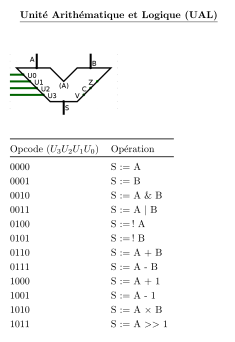
\includegraphics[width=\linewidth]{Figs/ual.pdf}\\\centering a)
   \end{minipage} \hfill
   \begin{minipage}[c]{.58\linewidth}
\includegraphics[width=\columnwidth]{Figs/ual_inner.pdf}\\\centering b)
   \end{minipage}
\caption{\label{fig:ual} a) Représentation d'une unité arithmétique et logique (UAL) disposant de $2^4 = 16$ poérations sélectionnables par l'entrée $U_3U_2U_1U_0$. Les opérandes $A$ et $B$ et la sortie $S$ sont codées ici sur 16 bits. Les signaux $N, Z, C, V$ sont les indicateurs d'états : (N: est la sortie est négative ?, Z: est ce que la sortie est nulle ? C : est ce que l'opération génère une retenue ? V: est ce que l'opération produit un dépassement de capacité. b) Une partie de l'organisation interne d'une UAL naïve avec des circuits effectuant chacune des opérations et un décodeur permettant d'en sélectionner une.}
\end{figure}

En TP, nous utiliserons des opérandes codées sur $16$ bits, donc $A$, $B$ et $S$ seront codés sur 16 bits. On représente sur la figure \ref{fig:ual}a une UAL avec $4$ bits pour sélectionner une opération (donc un total de $16$ opérations). Les signaux $N, Z, C, V$ sont les indicateurs d'états :
\begin{itemize}
\item $N$: est ce que la sortie est négative ?
\item $Z$: est ce que la sortie est nulle ?
\item $C$: est ce que l'opération génère une retenue ?
\item $V$: est ce que l'opération produit un dépassement de capacité ?
\end{itemize}
Une partie du schéma de l'UAL avec uniquement quelques opérations est représentée sur la figure \ref{fig:ual}b. Les 16 opérations sont sélectionnables par l'entrée $U$ et la table \ref{table:ual} donne le code de chacune des opérations.

\begin{table}[htbp]
\centering\begin{tabular}{c|ccc|c}
Code & Opération & & Code & Opération\\
\cline{0-1}
0000 & $S = A$ & & 1000 & $S = A+1$\\
0001 & $S = B$ & & 1001 & $S = A-1$\\
0010 & $S = A\& B$ & & 1010 & $S = A \times B$\\
0011 & $S = A|B$& &1011 & $S = A >> 1$\\
0100 & $S = \overline{A}$ & &1100 & \\
0101 & $S = \overline{B}$ & &1101 & \\
0110 & $S = A + B$ & & 1110 & \\
0111 & $S = A - B$& & 1111 & 
\end{tabular}
\caption{\label{table:ual} Exemple de code des opérations fournies par une UAL à $2^4 = 16$ opérations. Ici, seules $12$ opérations sont proposées; C'est l'UAL que nous utiliserons en TP. Pour ne pas confondre les opérations booléennes et arithmétiques sur des entiers, on note $A\&B$ le ET logique, $A|B$ le OU logique, $A+B$ l'addition. L'opération $A >> 1$ décale la représentation d'un bit sur la droite en complétant en tête par un $0$ ou un $1$ en fonction du premier bit. Sur des représentations en complément à deux, cette opération divise par deux la valeur de $A$.}
\end{table}

Il est important de retenir que l'unité arithmétique et logique n'a aucune idée du type des entrées. Les entrées $A$ et $B$ sont des paquets de bits à $0$ ou à $1$ et absolument pas des entiers, des booléens, etc... Pour le coup, il est tout à fait légitime de réaliser une opération logique sur ce que vous considérez être la représentation d'un entier. Par exemple, considérons l'opération $A\& B$ de code $U = 0010$ :
\begin{itemize}
\item avec $A = 3_{10} = 0\cdots 011$ et $B = 0\cdots 001$, on a $S = 0\cdots001$
\item avec $A= 2_{10} = 0\cdots 010$ et $B = 0\cdots 001$, on a $S= 0\cdots 000$
\end{itemize}
L'opération $A\&B$ avec $B= 0\cdots 001$ permet de tester la parité de $A$ ce qui peut être pratique si $A$ représente un entier.


%% \subsubsection{Multiplieur}



%% \begin{itemize}
%% \item table de vérité
%% \item Mentionner brièvement la combinaison de portes logiques éléments pour construire des circuits combinatoires plus compliqués, par exemple pour illustrer comment construire un additionneur, etc... vers l'UAL;
%% \item mentionner au moins le term de tableau de Karnaugh pour la synthèse
%% \item multiplex
%% \end{itemize}


\subsection{Unité arithmétique en virgule flottante}

La manipulation des représentations à virgule flottante nécessite un circuit dédié qui s'appelle Unité de calcul à virgule flottante (\emph{floating point unit}, FPU). Jusque dans les années 1990, le calcul en virgule flottante était réalisé par un processeur dédié, qui était optionnel, et indépendant du processeur ``principal'' comme par exemple les coprocesseurs Intel 8087, 80287, 80387, 80487 compagnons des processeurs Intel 8086, 80286, 80386 et 80486. De nos jours, la technologie permet d'intégrer des unités de calcul à virgule flottante directement avec le processeur principal. 

\begin{figure}[htbp]
\begin{center}
\includegraphics[width=0.5\columnwidth]{Figs/80386with387.JPG}
\end{center}
\caption{Le processeur principal Intel 80386 et son coprocesseur optionnel 80387 réalisant les opérations arithmétiques sur les représentations à virgule flottante. Source:Wikipedia.}
\end{figure}
%\todo{on peut écrire un algorithme de calcul sur les représentations flottantes avec un processeur ``principal''; quel est l'intérêt de faire un circuit dédié ??}

%%%%%%%%%%%%%%%%%%%%%%%%%%%%%%%%%%%%%%%%%%%%%%%%%%%%%%%%%%%%%%%

\pagebreak
\section{Circuits de logique séquentielle}

Dans les sections précédentes, nous avons présenté des circuits logiques dits ``combinatoires''. La sortie de ces circuits combinatoires à un instant $t$ dépends uniquement de ses entrées à ce même instant, il n'y a pas de dépendance à l'historique de la valeur des entrées\footnote{modulo les temps de propagation des signaux dans le circuit.}. Nous sommes à deux doigts de construire notre premier microprocesseur mais il nous manque encore un ingrédient. Imaginez, votre amie suzette est ornitologue, elle aimerait bien disposer d'un appareil électronique pour compter les oiseaux lors des migrations et si possible un appareil simple, par exemple avec deux boutons : un bouton pour réinitialiser le compteur et un bouton pour l'incrémenter d'une unité. Vous vous dites ``Super, je sais réaliser un additionneur, mettre une sortie à 0, c'est partie, j'écris la table de vérité''. Et là, vous êtes coincés, parce que pour une configuration d'entrée, par exemple ``bouton incrémenter pressé'', vous avez plusieurs sorties possibles : si il y avait 1 oiseau, il y en a désormais 2, mais si il y avait 2 oiseaux, il y en a désormais 3. Il vous faudrait disposer d'un moyen de représenter un \textbf{état} $n_o$ et qu'à l'appui sur le bouton vous puissiez \textbf{transiter} vers \textbf{l'état} $n_o + 1$. Dis dans l'autre sens, l'état courant dépends de l'entrée et également de l'état précédent. Cette idée est illustrée sur le schéma \ref{fig:intro_seq}. Il nous manque donc la brique permettant de mémoriser un état et c'est le sujet de cette partie.


\begin{figure}[htbp]
\centering\includegraphics[width=0.75\linewidth]{Figs/intro_seq.pdf}
\caption{\label{fig:intro_seq} Schéma de principe de n'importe quel système numérique. Etant donné un état courant et des entrées, on peut calculer des sorties et le prochain état qu'il suffit de mémoriser pour disposer d'un système dont l'influence des entrées dépends de l'état courant.}
\end{figure}



%\todo{Mentionner l'exemple de la mémoire mais peut être aussi d'un compteur}\\
%\todo{Le verrou D (D latch) peut se voir comme un mutiplexeur à 2 entrées dont l'une est sa sortie, l'autre est la donnée à mémoriser}\\

%% \subsection{Logique séquentielle synchrone et asynchrone}

%% Le verrou (\emph{latch}) est asynchrone (pas de signal d'horloge); la bascule (\emph{flip-flop}) est synchrone (avec un signal d'horloge). 

\subsection{Verrou/Bascule RS}

Le verrou RS (\emph{Reset}/\emph{Set}) possède deux entrées ($S$, $R$) et deux sorties ($Q,\bar{Q}$) comme illustré sur la figure \ref{fig:verrou_rs}. Le circuit contient des boucles de rétroaction et sa sortie est dépendante de l'historique de ses entrées comme nous allons le voir.

\begin{figure}[htbp]
\begin{center}
\tikzstyle{branch}=[fill,shape=circle,minimum size=3pt,inner sep=0pt]
\begin{tikzpicture}[label distance=2mm]

    \node[nor gate US, draw, logic gate inputs=nn] at (0,0) (Nor1) {};
    \node[nor gate US, draw, logic gate inputs=nn] at (0,-2) (Nor2) {};

    \node (S) at ($(Nor1.input 1) - (1,0)$) {$Set$};
    \node (R) at ($(Nor2.input 2) - (1,0)$) {$Reset$};
    \node (bQ) at ($(Nor1.output) + (1, 0)$) {$\bar{Q}$};
    \node (Q) at ($(Nor2.output) + (1, 0)$) {$Q$};

    \node at ($(Nor1.output) - (0.5,0)$) {$1$};
    \node at ($(Nor2.output) - (0.5,0)$) {$2$};

    \draw (S) -- (Nor1.input 1);
    \draw (Nor2.output) -- ([xshift=0.5cm]Nor2.output) -- ++(0, 0.5) -- ([xshift=-0.5cm,yshift=-0.5cm]Nor1.input 2) -- ([xshift=-0.5cm]Nor1.input 2) -- (Nor1.input 2);
    \draw (Nor1.output) -- (bQ);

    \draw (R) -- (Nor2.input 2);
    \draw (Nor1.output) -- ([xshift=0.5cm]Nor1.output) -- ++(0, -0.5) -- ([xshift=-0.5cm,yshift=+0.5cm]Nor2.input 1) -- ([xshift=-0.5cm]Nor2.input 1) -- (Nor2.input 1);
    \draw (Nor2.output) -- (Q);
\end{tikzpicture}
\end{center}
\caption{\label{fig:verrou_rs} Un verrou RS (Reset/Set) formé par deux portes NOR (les numéros dans les portes facilitent l'explication du fonctionnement du circuit) avec des connections réentrantes.}
\end{figure}

Étudions le comportement du verrou pour les entrées $(0,0)$, $(0,1)$, et $(1,0)$, on verra un peu plus loin que l'entrée $(1,1)$ conduit à un état instable et qu'on s'interdira donc cette entrée. La figure~\ref{fig:chrono_rs_1} présente l'évolution au cours du temps des entrées et des sorties du verrou. A l'instant $t_0$, l'entrée passe de $(R,S) = (0,0)$ à $(R,S) = (0,1)$. Il existe une période transitoire entre $t_0$ et $t_0 + \Delta$ avant que le circuit n'atteigne un état stable. En effet, à $t_0$, lorsque $S$ passe à $1$, seules les entrées de la première porte NOR changent. Ses entrées étant $(S, Q) = (1,0)$, la sortie passe à $\bar{Q} = 0$. Cela affecte alors à $t_0 + \Delta/2$ la deuxième porte NOR qui, ayant ses entrées à $(\bar{Q}, R) = (0,0)$ voit sa sortie passer à $Q = 1$ après un délai de $\Delta /2$. Au temps $t_0+\Delta$, les sorties du verrou sont alors à $(Q,\bar{Q}) = (1, 0)$ qui est un état stable pour le circuit. Le délai $\Delta/2$ corresponds au temps de propagation des signaux dans les portes logiques NOR et est de l'ordre de quelques dizaines à centaines de nanosecondes\footnote{Voir par exemple la notice technique de la puce 74HC02 ou CD4001}. \\

\begin{figure}[htbp]
\begin{center}
\begin{tikztimingtable}[
    timing/coldist=2pt,     % column distance
    xscale=1,yscale=1, % scale diagrams
    semithick               % set line width
]
$R$       & 2L       LLLLLL       LLLLLL       HHHHHH       LLLLLL  \\
$S$       & 2L       HHHHHH       LLLLLL       LLLLLL       LLLLLL  \\
$Q$       & 2L       LLHHHH       HHHHHH       HLLLLL       LLLLLL\\
$\bar{Q}$ & 2H N(Q1) HLLLLL N(Q2) LLLLLL N(Q3) LLHHHH N(Q4) HHHHHH \\
          & SS       SSSSSS       SSSSSS       SSSSSS       SSSSSS\\
\extracode
  %\tablerules
  %\tablegrid
  \begin{pgfonlayer}{background}
    \vertlines[help  lines]{2,4,8,14,16,20}
    \draw[thick,<->,shorten >=2pt,shorten <=2pt,>=stealth] (2, -8) -- (4,-8);
    \draw [anchor=mid] node at (3,-7) {\tiny $\Delta$};
    \draw [anchor=north] let \p1=(Q1) in node at (\x1,-9) {$t_0$};

    \draw [anchor=north] let \p1=(Q2) in node at (\x1,-9) {$t_1$};

    \draw[thick,<->,shorten >=2pt,shorten <=2pt,>=stealth] (14, -8) -- (16,-8);
    \draw [anchor=mid] node at (15,-7) {\tiny $\Delta$};
    \draw [anchor=north] let \p1=(Q3) in node at (\x1,-9) {$t_2$};

    \draw [anchor=north] let \p1=(Q4) in node at (\x1,-9) {$t_3$};
  \end{pgfonlayer}
\end{tikztimingtable}
\end{center}
\caption{\label{fig:chrono_rs_1} Chronogramme d'un verrou RS.}
\end{figure}

A l'instant $t_1$, les entrées repassent à $(R,S) = (0,0)$. Les entrées de la première porte NOR étant $(S, Q) = (0, 1)$, la sortie reste à $\bar{Q} = 0$. Pour la deuxième porte, il en est de même; ses entrées étant $(\bar{Q}, R) = (0, 0)$, sa sortie reste à $\bar{Q} = 1$. Cet état est un état de mémorisation, le verrou reste dans l'état dans lequel il était. \\

Passons maintenant, à l'instant $t_3$, les entrées à $(R,S) = (1,0)$. Seule la deuxième porte NOR voit ses entrées changer pour le moment et passer à $(\bar{Q}, R) = (0, 1)$, sa sortie passe donc à $Q = 0$. Cela a pour conséquence d'affecter la première porte; ayant les entrées $(S, Q) = (0, 0)$, sa sortie passe à $\bar{Q} = 1$. Cet état est un état stable. \\

 La table de vérité du verrou $RS$ est donnée ci-dessous~:\\
\begin{center}
\begin{tabular}{cc||ccl}
$R$ & $S$ & $Q$ & $\bar{Q}$ & Remarque\\
\hline
0 & 0 & $x$ & $\bar{x}$ & Maintien de l'état précédent\\
0 & 1 & 1 & 0 & Mise à un\\
1 & 0 & 0 & 1 & Mise à zéro\\
1 & 1 & 0 & 0 & Etat interdit 
\end{tabular}
\end{center}

\begin{framed}
\textbf{Résumé : } Un verrou RS ne s'utilise que pour les entrées $(R,S) \in \{(0,0), (0,1), (1,0)\}$.
\begin{itemize}
\item l'entrée $R=0$, $S=1$ met à 1 la sortie du verrou $Q = 1$, $\bar{Q}=0$,
\item l'entrée $R=1$, $S=0$ met à 0 la sortie du verrou $Q = 0$, $\bar{Q}=1$,
\item l'entrée $R=0$, $S=0$ laisse la sortie du verrou dans son état
\end{itemize}
\end{framed}

% 
% http://www.iitg.ernet.in/asahu/cs221/Lects/Lec13.pdf
Si les entrées $R$ et $S$ sont simultanément à un niveau haut, le système entre dans un état pour lequel les sorties $Q$ et $\bar{Q}$ ne sont pas complémentaires et est considéré comme un état interdit. En effet, le verrou peut alors entrer dans un régime instable. Si les entrées $R$ et $S$ repassent simultanément à un niveau bas $(R, S) = (0,0)$ alors que les sorties étaient également à l'état bas $(Q, \bar{Q}) = (0,0)$, dans le cas d'un circuit tout à fait symétrique, les sorties vont passer à $(1,1)$ puis $(0,0)$, ... En pratique, le circuit n'est pas parfaitement symétrique parce que les portes (et leur délais de propagation) ne sont pas tout à fait identiques et les connexions entre les sorties et les entrées non plus. Cette asymétrie conduira alors le verrou à atteindre un état stable mais en un temps arbitrairement long et il finira dans un état impossible à prédire. C'est la raison pour laquelle l'entrée $(R,S) = (1,1)$ est interdite.\\


\paragraph{Exemple : mémoriser l'appui d'un bouton:\\}

Pour illustrer l'effet mémoire d'un verrou RS, considérons deux circuits représentés sur les figures \ref{fig:ill_verrou}a et \ref{fig:ill_verrou}b. Sur la figure \ref{fig:ill_verrou}a, nous avons simplement un interrupteur qui contrôle l'allumage d'une lumière. Si on appuis sur le bouton, la lumière s'allume mais dés qu'on relâche le bouton, la lumière s'éteint. Si on modifie un peu le circuit pour placer un verrous R/S qu'on peut contrôler avec deux boutons ``allume'' et ``éteint'', on peut maintenir la lumière allumée même lorsque le bouton ``allume'' est relâché. On a donc bien mémorisé l'état ``allumé''. 

\begin{figure}[htbp]
\begin{tabular}{cc}
\begin{circuitikz}
\draw[color=black, thick]
    (0,0) to [push button,l=allume] (1.5, 0) to [lamp] (3.0, 0) to [R] (4.5, 0) to (5, 0) node[ground] {}
    (0,0) to [short,-o](0, 2) node[right]{$V^+$};
\end{circuitikz}&
\begin{circuitikz}[scale=0.9,transform shape]
\draw[color=black, thick]
    (4,0.1) node[nor gate US, draw, logic gate inputs=nn] (Nor2) {}
    (4,2.1) node[nor gate US, draw, logic gate inputs=nn] (Nor1) {}
    (0,0) to [push button,l=éteint] (2, 0) to (Nor2.input 2)
    (0,2.2) to [push button,l=allume] (2, 2.2) to (Nor1.input 1)  
    (Nor2.output) to [R] ([xshift=2.5cm]Nor2.output) to [lamp] ([xshift=3.5cm]Nor2.output) to ([xshift=4cm]Nor2.output) node[ground]{}
    (0,0) to [short,-o](0,3) node[above]{$V^+$}
    (Nor1.output) to ([xshift=.5cm]Nor1.output) node(Nor1o) {} to ([yshift=-0.5cm]Nor1o) to ([xshift=-.5cm,yshift=.5cm]Nor2.input 1) to ([xshift=-.5cm]Nor2.input 1) to (Nor2.input 1)
    (Nor2.output) to ([xshift=.5cm]Nor2.output) node(Nor2o) {} to ([yshift=0.5cm]Nor2o) to ([xshift=-.5cm,yshift=-.5cm]Nor1.input 2) to ([xshift=-.5cm]Nor1.input 2) to (Nor1.input 2)
    ([xshift=-1cm]Nor1.input 1) to [R, bipoles/length=0.5cm] ([xshift=-1cm,yshift=-1cm]Nor1.input 1) |- ([xshift=-1.5cm,yshift=-1cm]Nor1.input 1) node[ground,rotate=-90](gndpulldown) {}
    ([xshift=-1cm]Nor2.input 2) to [R, bipoles/length=0.5cm] ([xshift=-1cm,yshift=1cm]Nor2.input 2) |- (gndpulldown);
\end{circuitikz}\\
a) & b)
\end{tabular}
\caption{\label{fig:ill_verrou}a) Si le bouton est appuyé, la lumière s'allume; Si le bouton est relâché, la lumière s'éteint. b) Avec un verrou R/S, si on appuis sur le bouton ``allume'', la lumière s'allume et reste allumé même si on relâche le bouton. La lumière s'éteindra en pressant sur le bouton ``éteint''.}
\end{figure}




 L'un des inconvénients du verrou RS est que son état est tout de même très dépendant de ses entrées $R$ et $S$ puisque seul l'état $(R,S) = (0,0)$ est un état de mémoire. Il est souvent préférable d'avoir plus de contrôle sur les instants o{\`u} l'on souhaite mémoriser une donnée (fournie par R et S). On définit alors le verrou RS contrôlé (\emph{gated RS latch}) comme sur la figure~\ref{fig:gated_verrou_rs}. La seule différence avec le verrou RS est l'introduction d'un signal de contrôle qui force les entrées des portes NOR provenant de $R$ et $S$ à un niveau bas lorsque $Enable = 0$. Si $Enable=1$, ce circuit se comporte comme un verrou RS.


\begin{figure}[htbp]
\begin{center}
\tikzstyle{branch}=[fill,shape=circle,minimum size=3pt,inner sep=0pt]
\begin{tikzpicture}[label distance=2mm]

    \node[nor gate US, draw, logic gate inputs=nn] at (0,0) (Nor1) {};
    \node[nor gate US, draw, logic gate inputs=nn] at (0,-2) (Nor2) {};
    \node[and gate US, draw, logic gate inputs=nn] at ($(Nor1.input 1) - (1, 0)$) (And1) {};
    \node[and gate US, draw, logic gate inputs=nn] at ($(Nor2.input 2) - (1, 0)$) (And2) {};

    \node[anchor=east] (S) at ($(And1.input 1) - (1,0)$) {$Set$};
    \node[right] (E) at (-4,-1) {$Enable$};
    \node[anchor=east] (R) at ($(And2.input 2) - (1,0)$) {$Reset$};
    \node (bQ) at ($(Nor1.output) + (1, 0)$) {$\bar{Q}$};
    \node (Q) at ($(Nor2.output) + (1, 0)$) {$Q$};

    \node at ($(Nor1.output) - (0.5,0)$) {};
    \node at ($(Nor2.output) - (0.5,0)$) {};

    \draw (S) -- (And1.input 1);
    \draw (And1.output) -- (Nor1.input 1);
    \draw (R) -- (And2.input 2);
    \draw (And2.output) -- (Nor2.input 2);
    \draw (E) -| ($(And1.input 2)-(0.5,0)$) -- (And1.input 2);
    \draw (E) -| ($(And2.input 1)-(0.5,0)$) -- (And2.input 1);



    \draw (Nor2.output) -- ([xshift=0.5cm]Nor2.output) -- ++(0, 0.5) -- ([xshift=-0.5cm,yshift=-0.5cm]Nor1.input 2) -- ([xshift=-0.5cm]Nor1.input 2) -- (Nor1.input 2);
    \draw (Nor1.output) -- (bQ);

    \draw (Nor1.output) -- ([xshift=0.5cm]Nor1.output) -- ++(0, -0.5) -- ([xshift=-0.5cm,yshift=+0.5cm]Nor2.input 1) -- ([xshift=-0.5cm]Nor2.input 1) -- (Nor2.input 1);
    \draw (Nor2.output) -- (Q);
\end{tikzpicture}
\end{center}
\caption{\label{fig:gated_verrou_rs}Verrou RS contrôlé (\emph{gated RS latch}).}
\end{figure}

Ce verrou fonctionne sur des niveaux du signal de contrôle : lorsque le signal de contrôle \emph{enable} est à l'état haut, on retrouve un verrou RS et lorsque le signal de contrôle \emph{enable} est à l'état bas le verrou est dans un état de mémoire, peu importe ce qui se passe sur ses entrées (cf fig.\ref{fig:chrono_gated_rs_1}).

\begin{figure}[htbp]
\begin{center}
\begin{tikztimingtable}[
    timing/coldist=2pt,     % column distance
    xscale=1,yscale=1, % scale diagrams
    semithick               % set line width
]
$E$       & LH       HHHHHH       HHHLLL       LLLLLL       LLLLLL \\
$R$       & 2L       LLLLLL       LLLLLL       HHHHHH       LLLLLL  \\
$S$       & 2L       HHHHHH       LLLLLL       LLLLLL       LLLLLL  \\
$Q$       & 2L       LLHHHH       HHHHHH       HHHHHH       HHHHHH \\
$\bar{Q}$ & 2H N(Q1) HLLLLL N(Q2) LLLLLL N(Q3) LLLLLL N(Q4) LLLLLL \\
          & SS       SSSSSS       SSSSSS       SSSSSS       SSSSSS\\
\extracode
  %\tablerules
  %\tablegrid
  \begin{pgfonlayer}{background}
    \vertlines[help  lines]{2,4,8,14}
    \draw[thick,<->,shorten >=2pt,shorten <=2pt,>=stealth] (2, -10) -- (4,-10);
    \draw [anchor=mid] node at (3,-9) {\tiny $\Delta$};
    \draw [anchor=north] let \p1=(Q1) in node at (\x1,-10) {$t_0$};

    \draw [anchor=north] let \p1=(Q2) in node at (\x1,-10) {$t_1$};

    \draw [anchor=north] let \p1=(Q3) in node at (\x1,-10) {$t_2$};
  \end{pgfonlayer}
\end{tikztimingtable}
\end{center}
\caption{\label{fig:chrono_gated_rs_1} Chronogramme d'un verrou RS contrôlé.}
\end{figure}



%Le verrou RS (\emph{RS-latch}) est un circuit asynchrone: le changement de la sortie est commandé par le changement des entrées $R$ et $S$. Parfois, on souhaite contrôler 

% A voir sur les bascules D : http://www.eng.auburn.edu/~strouce/class/elec2200/elec2200-9.pdf

%\textbf{Illustration avec une mémoire 2 nor + 2 leds + 2 boutons sous logisim}

\subsection{Verrou D}

Nous sommes presque arrivé à la réalisation d'une mémoire à un bit. On souhaite mémoriser un bit, notons le $D$. Il suffit alors de considérer le verrour RS en connectant convenablement les entrées Set et Reset à $D$ comme sur la figure \ref{fig:verrou_d}

\begin{figure}[htbp]
   \begin{minipage}[c]{.7\linewidth}
\tikzstyle{branch}=[fill,shape=circle,minimum size=3pt,inner sep=0pt]
\begin{tikzpicture}[label distance=2mm]

    \node[nor gate US, draw, logic gate inputs=nn] at (0,0) (Nor1) {};
    \node[nor gate US, draw, logic gate inputs=nn] at (0,-2) (Nor2) {};
    \node[and gate US, draw, logic gate inputs=nn] at ($(Nor1.input 1) - (1, 0)$) (And1) {};
    \node[and gate US, draw, logic gate inputs=nn] at ($(Nor2.input 2) - (1, 0)$) (And2) {};
    \node[not gate US, draw] at ($(And2.input 2) - (1,0)$) (Not) {};

    \node (D) at ($(And1.input 1) - (4,0)$) {$D$};

    \node[right] (E) at (-6,-1) {$Enable$};
    \node (bQ) at ($(Nor1.output) + (1, 0)$) {$\bar{Q}$};
    \node (Q) at ($(Nor2.output) + (1, 0)$) {$Q$};

    \node at ($(Nor1.output) - (0.5,0)$) {};
    \node at ($(Nor2.output) - (0.5,0)$) {};

    \draw (D) -- (And1.input 1) node [midway,circ] (S) {};
    \draw (S) |- (Not.input);

    \draw (And1.output) -- (Nor1.input 1);
    \draw (Not.output) -- (And2.input 2);
    \draw (And2.output) -- (Nor2.input 2);
    \draw (E) -| ($(And1.input 2)-(0.5,0)$) node[midway,circ]{} -- (And1.input 2);
    \draw (E) -| ($(And2.input 1)-(0.5,0)$) -- (And2.input 1);



    \draw (Nor2.output) -- ([xshift=0.5cm]Nor2.output) -- ++(0, 0.5) -- ([xshift=-0.5cm,yshift=-0.5cm]Nor1.input 2) -- ([xshift=-0.5cm]Nor1.input 2) -- (Nor1.input 2);
    \draw (Nor1.output) -- (bQ);

    \draw (Nor1.output) -- ([xshift=0.5cm]Nor1.output) -- ++(0, -0.5) -- ([xshift=-0.5cm,yshift=+0.5cm]Nor2.input 1) -- ([xshift=-0.5cm]Nor2.input 1) -- (Nor2.input 1);
    \draw (Nor2.output) -- (Q);
\end{tikzpicture}\\\centering a)
\end{minipage}\hfill
\begin{minipage}[c]{.1\linewidth}
\includegraphics[width=\columnwidth]{Figs/verrou_D.pdf}
\\\centering b)
\end{minipage}
\caption{\label{fig:verrou_d} a) Un verrou D (\emph{Data-latch}) construit à partir d'un verrou RS en connectant les entrées Reset et Set : $Set = D, Reset = \overline{D}$. b) Représentation schématique d'un verrou D.}
\end{figure}

Ce circuit assure aussi que l'état instable du verrou $RS$ obtenu avec les entrées $R=1, S=1$ n'est jamais obtenu puisque les entrées $R$ et $S$ son câblées pour être complémentaires.

\begin{framed}
\textbf{Résumé : } Un verrou D a deux entrées $Date$ et $Enable$ et fonctionne de la manière suivante :
\begin{itemize}
\item si l'entrée $E=1$, alors $Q = D$, on dit que le verrou est transparent,
\item si l'entrée $E=0$, alors le verrou est dans un état mémoire, sa sortie ne changera pas si $D$ change et ne pourra changer que si $E$ passe à l'état haut
\end{itemize}
\end{framed}



\subsection{Systèmes logiques synchrones : horloge et fronts montants}

On précisait en introduction que le but du circuit mémoire que nous cherchons à construire est de mémoriser l'état courant d'un système, peu importe ce que représente cet état. On comprends bien que le verrou D recevra sur l'entrée D l'état mais qu'en est-il de l'entrée Enable ? On va ici considérer que la transition d'un état à un autre est rythmée par une horloge (un signal périodique en créneaux) et cela va nous conduire à construire des \emph{systèmes logiques synchrones}. Lorsque les transitions d'état sont produites par les entrées, sans être dépendantes d'un signal d'horloge, on parle de \emph{systèmes logiques asynchrones} mais nous n'en parlerons pas ici. 

Donc, pour nous, c'est une horloge qui va dicter les instants auxquels un système peut changer d'état. Un signal d'horloge est représenté sur la figure \ref{fig:clk}. Ce signal est périodique de période $T$ et de fréquence $f = 1/T$.

\begin{figure}[htbp]
\begin{center}
\begin{tikztimingtable}[
    timing/coldist=2pt,     % column distance
    xscale=1,yscale=1, % scale diagrams
    semithick               % set line width
]
$Horloge$       & 12{2C} C\\
& \\
\extracode
  %\tablerules
  %\tablegrid
  \begin{pgfonlayer}{background}
    \vertlines[help  lines]{2,6}
    \draw[thick,<->,shorten >=2pt,shorten <=2pt,>=stealth] (2, -3) -- (6,-3);
    \draw [anchor=mid] node at (4,-2) {$T$};
  \end{pgfonlayer}
\end{tikztimingtable}
\end{center}
\caption{\label{fig:clk} Un signal d'horloge est un signal en créneaux, périodique de période $T$ et de fréquence $f = 1/T$.}
\end{figure}

Si on utilise directement ce signal d'horloge comme entrée $Enable$ à un verrou D, le verrou est transparent sur le niveau haut de l'horloge comme illustré sur la figure \ref{fig:chrono_verrou_D}.

\begin{figure}[htbp]
\begin{center}
\begin{tikztimingtable}[
    timing/coldist=2pt,     % column distance
    xscale=1,yscale=2, % scale diagrams
    semithick               % set line width
]
$Horloge$ & 8L 8H 8L 8H \\
$D$       & 2L 3H 2L 2H  1L 2H 1L 1H 1L 3H  6L   2L 3H 3L \\
$Q$       & 8L 1H 1L 2H 1L 1H 1L 9H    2L 3H 3L\\
\extracode
  %\tablerules
  %\tablegrid
\end{tikztimingtable}
\end{center}
\caption{\label{fig:chrono_verrou_D} Chronogramme d'un verrou D contrôlé par une horloge. La sortie du verrou est autorisé à changer (il est transparent) tant que le signal d'horloge est au niveau haut.}
\end{figure}


Pour s'assurer qu'une seule transition ait lieu, il faut garantir que la mise à jour de la mémoire ne se fasse qu'à des instants particuliers, comme par exemple le front montant de l'horloge\footnote{on pourrait aussi considérer le front descendant de l'horloge}, lorsque ce signal passe du niveau bas $0$ au niveau haut $1$ (fig. \ref{fig:clk_fronts}). En chaînant deux verrous D, on construit ce qu'on appelle la bascule D maître escale pour laquelle on est assuré que la mise à jour de la sortie n'a lieu que sur un front d'horloge.

\begin{figure}[htbp]
\centering\includegraphics[width=0.5\linewidth]{Figs/clk_fronts.pdf}
\caption{\label{fig:clk_fronts} Le front montant d'un signal créneau est lorsque ce signal passe du niveau bas $0$ au niveau haut $1$. Le front descendant est lorsque le signal passe du niveau haut au niveau bas.}
\end{figure}

\subsection{Bascule D synchrone sur front montant : maître esclave}

En chaînant deux verrous D, on peut construire une mémoire mise à jour sur le front montant d'un signal d'horloge comme illustré sur la figure \ref{fig:flipflop_d}.

\begin{figure}[htbp]
   \begin{minipage}[c]{.7\linewidth}
\includegraphics[width=\columnwidth]{Figs/flipflop_D.pdf}\\\centering a)
\end{minipage}\hfill
\begin{minipage}[c]{.2\linewidth}
\includegraphics[width=\columnwidth]{Figs/flipflop_D_schema.pdf}
\\\centering b)
\end{minipage}
\caption{\label{fig:flipflop_d} a) Une bascule D (\emph{Data-flipflop}) construite à partir de deux verrous D respectivement appelés maître et esclave, dont la mise à jour n'est permise que sur un front montant d'horloge. b) Représentation schématique d'une bascule D. Le symbole en triangle indique un composant sensible au front montant d'horloge. Si il avait été sensible au front descendant, on aurait ajouté un petit cercle devant le triangle, à l'extérieur du composant (comme sur les portes inverseur).}
\end{figure}

Reprenons les entrées (D et Horloge) de la figure \ref{fig:chrono_verrou_D} et traçons le chronogramme des sorties des deux verrous sur la figure \ref{fig:chrono_flipflop_d}. Sur ce chronogramme, les entrées et sorties des deux verrous sont suffixés du numéro du verrou : $D_1$,$E_1$, $Q_1$ pour le premier verrou, le verrou maître et $D_2$, $E_2$ et $Q_2$ pour le second verrou, le verrou escale. Pour comprendre le fonctionnement de ce circuit, il suffit de considérer chacun des verrous l'un après l'autre en commençant par identifier quand les signaux Enable de chacun des verrous est à l'état haut et en recopiant l'entrée dans ce cas. Lorsque le signal Enable est à l'état bas, le verrou est dans l'état mémoire. Au final, si on ne se concentre que sur les entrées $D$, $Horloge$ et la sortie $Q = Q_2$, on constate que la sortie est une copie de l'entrée aux fronts montants de l'horloge, nous avons donc construit un circuit mémoire mis à jour sur les fronts montants de l'horloge (\emph{edge-triggered flip flop}).

\begin{figure}[htbp]
\begin{center}
\begin{tikztimingtable}[
    timing/coldist=2pt,     % column distance
    xscale=1,yscale=2, % scale diagrams
    semithick               % set line width
]
$Horloge$ & 8L 8H 8L 8H \\
$D=D_1$       & 2L 3H 2L 2H  1L 2H 1L 1H 1L 3H  6L   2L 3H 3L \\
$E_1$     & 8H 8L 8H 8L\\
$Q_1=D_2$     & 2L 3H 2L 1H 8H 2H 6L 8L\\
$E_2$     & 8L 8H 8L 8H\\
$Q=Q_2$       & 8L 8H 8H 8L\\
\extracode
  %\tablerules
  %\tablegrid
\end{tikztimingtable}
\end{center}
\caption{\label{fig:chrono_flipflop_d} Chronogramme d'une bascule D maître-escale sensible à un front montant d'horloge. La sortie de la bascule est la valeur de l'entrée $D$ au dernier front montant d'horloge.}
\end{figure}

Nous n'étudierons pas plus en détails le fonctionnement de la bascule D, sachez simplement qu'en pratique, le bon fonctionnement de la bascule est garantie si l'entrée est stable autour du front montant d'horloge, encadré par des temps de mise en place (\emph{setup time}) et de maintien (\emph{hold time}).

\subsection{Réalisation d'un verrou D avec un mutliplexeur}
\label{subsec:verrouD_multiplexeur}

Une autre réalisation possible d'un verrou peut se construire à partir d'un multiplexeur 2-1. Je vous rappelle qu'un multiplexeur à 2 entrées, un bit de sélection et une sortie peut être vu comme un aiguillage. Pour réaliser un verrou D avec un multiplexeur, il suffit de reboucler la sortie du multiplexeur sur la première entrée de telle sorte que si le bit de sélection vaut $0$, le circuit soit dans un état mémoire et de présenter l'entrée $D$ comme deuxième entrée du multiplexeur de telle sorte que le circuit soit transparent lorsque le bit de sélection vaut $1$. Il faudra néanmoins faire attention à utiliser la réalisation du multiplexeur sans aléas statiques. En effet, avec le multiplexeur ayant un aléa statique, si $S=1$, $D=1$ et $Q=1$, lorsque le multiplexeur est basculé dans l'état mémoire $S=1 \rightarrow S=0$, l'aléa de sortie conduit à oublier $Q=1$ et à mémoriser $Q=0$.

\subsection{Registre et mémoire RAM (Random Access Memory)}

\subsubsection{Registre à $n$ bits sur front montant}

La bascule D (maître-escale par exemple) permet de mémoriser un bit d'information et est mise à jour sur un front montant d'horloge. Pour pouvoir mémoriser un mot de plus de $n$ bits, il suffit de considérer $n$ bascules D et de construire ce qu'on appelle \textbf{un registre à n bits}, représenté sur la figure \ref{fig:registre}. Les entrées $Enable$ et $Clear$ apparaissent parfois. L'entrée $Enable$ permet d'autoriser le registre à se mettre à jour. Si l'entrée Enable est à $0$, aucune mise à jour du contenu du registre n'aura lieu. L'entrée Clear permet de remettre à $0$ le contenu du registre $Q=000\cdots$ de manière asynchrone, i.e. sans attendre de front montant d'horloge.

\begin{figure}[htbp]
   \begin{minipage}[c]{.2\linewidth}
\includegraphics[width=\columnwidth]{Figs/registre.pdf}\\\centering a)
\end{minipage}\hfill
\begin{minipage}[c]{.4\linewidth}
\includegraphics[width=\columnwidth]{Figs/registre_inner.pdf}
\\\centering b)
\end{minipage}
\caption{\label{fig:registre} a) Un registre actif sur front montant à $n$ bits. Les entrées $E$ et $Clear$ sont parfois disponibles. L'entrée $E$ autorise la mise à jour du registre et doit être au niveau haut pour que les signaux d'horloge soient opérants. L'entrée Clear permet de remettre à $0$ de manière asynchrone le contenu du registre. b) Un registre à $n$ bits sur front montant peut se construire à l'aide de $n$ bascules D sur front montant.}
\end{figure}


\subsubsection{Mémoire en lecture et écriture (RAM)}

Au même titre que combiner $n$ bascules $D$ permet de mémoriser un mot de $n$ bits, on peut aussi combiner $2^k$ registres pour mémoriser $2^k$ mots de $n$ bits comme sur la figure \ref{fig:ram}. Pour l'écriture, l'activation de l'un ou l'autre des registres se fait par l'entrée $Enable$ alimentées par la sortie d'un décodeur. Pour la lecture, le registre sélectionné par l'adresse est dirigé en sortie grâce à un multiplexeur. On dispose alors d'un contenu dit adressable. En effet l'entrée $Adr$ de $k$ bits permet de sélectionner l'un ou l'autre des $2^k$ registres soit en écriture, soit en lecture. Le choix entre l'écriture et la lecture se fait par des entrées supplémentaires Load et Store (parfois combinées en une seule).

\begin{figure}[htbp]
   \begin{minipage}[c]{.4\linewidth}
\includegraphics[width=\columnwidth]{Figs/ram.pdf}\\\centering a)
\end{minipage}\hfill
\begin{minipage}[c]{.4\linewidth}
\includegraphics[width=\columnwidth]{Figs/ram_inner.pdf}
\\\centering b)
\end{minipage}
\caption{\label{fig:ram} a) Illustration schématique d'une RAM de capacité $n 2^k$ disposant d'une entrée $D_i$ et d'une sortie $D_o$ sur $n$ bits : l'une pour le stockage l'autre pour le chargement, d'une ligne d'adresse sur $k$ bits, d'un signal d'horloge, et de signaux de contrôle pour autoriser le chargement ou le stockage de données. b) Une partie de l'organisation interne d'une RAM. Il manque sur ce schéma le circuit permettant de piloter le chargement (load) et le stockage (store) des données. }
\end{figure}

On distingue deux opérations avec les mémoires RAM : le chargement (load) et le stockage (store). Le chargement vise à placer sur le bus de données de sortie $D$, la valeur du contenu du registre adressé par l'entrée $Adr$. Le stockage vise à modifier le contenu du registre adressé par l'entrée $Adr$ avec la valeur présente sur le bus d'entrée $D$. Pour charger une valeur sur le bus de sortie il faudra :
\begin{itemize}
\item placer sur le bus d'adresse l'adresse du mot à lire
\item le mot à l'adresse $Adr$ est directement accessible sur le bus de sortie
\end{itemize}

Pour stocker une nouvelle valeur dans la mémoire, il faudra :
\begin{itemize}
\item placer sur le bus d'adresse l'adresse du mot à écrire
\item placer sur le bus de données la valeur à stocker
\item déclencher un front montant d'horloge et la nouvelle valeur sera stockée en mémoire
\end{itemize}

On parle de mémoire RAM (\emph{Random Access Memory}) puisque le temps d'accès en lecture/écriture d'un mot à une adresse donnée est indépendant de l'adresse.


%\textbf{Illustration du rôle de la bascule D : le registre à décalage}\\
%\textbf{Illustration avec le compteur par incrément : 2 bascules D avec rebouclage}\\



\vfill
\pagebreak

%%%%%%%%%%%%%%%%%%%%%%%%%%%%%%%%%%%%%%%%%%%%%%%%%%%%%%%%%%%%%%%

\section{Une première architecture interne simple d'un microprocesseur}

On dispose désormais de tout les éléments nécessaires à la réalisation d'un système de représentation et traitement d'informations numériques. La figure \ref{fig:premier_chemin_logisim} représente ce qu'on appelle un chemin de données dans lequel on reconnaît: 
\begin{itemize}
\item une unité arithmétique et logique dont les codes d'opération sont précisé dans la table~\ref{table:ual}
\item quatre registres (A, B, RADM et PC)
\item une RAM
\end{itemize}


\begin{figure}[htbp]
\includegraphics[width=\columnwidth]{Figs/premier_chemin_donnees.pdf}
\caption{\label{fig:premier_chemin_logisim} Un premier chemin de données consistué de quatre registres (A, B, RADM, PC), d'une Unité Arithmétique et Logique ainsi que de signaux de contrôles UAL, SetB, ReadB, .. tel qu'il se présente sous Logisim. La RAM est considérée comme un exemple externe au chemin de données et y est connecté par un bus d'adresse et un bus de données}
\end{figure}

Ce qu'on appelle chemin de données est l'ensemble des éléments qui permettent de traiter des informations, la RAM n'en fait pas partie en toute rigueur et doit être considéré comme un composant extérieur au chemin de données. Les données et donc la taille des bus A, B et S sont de 16 bits. Les adresses sont également codées sur 16 bits de telle sorte que la RAM contient $16 \times 2^{16}$ bits = $128$ Koctets. Ce chemin de données est celui que nous utiliserons en TP et c'est également celui que nous allons développer tout au long de ce cours pour lui ajouter quelques fonctionnalités. Les architectures actuelles utilisent de l'ordre de 8 à 32 registres internes, certains ayant des fonctions particulières et la RAM de l'ordre de quelques gigaoctets, les données et adresses étant codés sur 64 bits. 

\subsection{Registres internes : accumulateurs, registre d'adresse et compteur ordinal}

Les registres A et B vont servir à stocker les opérandes et résultats des opérations de l'UAL. Pour effectuer une opération sur des données stockées en mémoire, on s'arrangera toujours pour charger les opérandes dans les registres A et B, d'effectuer l'opération et de stocker le résultat dans un de ces deux registres et de stocker ensuite le résultat en RAM. C'est ce qu'on appelle une architecture Load/Store\footnote{qu'on oppose aux architectures registre-mémoire par exemple pour lesquelles on s'autorise à effectuer des opérations arithmétiques avec une opérande en RAM et une opérande en registre} : seules les opérations de chargement (LOAD) et de sauvegarde (STORE) accèdent à la RAM. Les opérations arithmétiques, par exemple, ne prendront jamais d'opérande directement de la RAM. C'est un choix de conception qu'on comprendra un peu plus tard.

Deux registres vont nous permettre d'accéder à la RAM : le \emph{program counter} (PC) et le \emph{registre d'adresse mémoire} (RADM). Le registre d'adresse mémoire permet de savoir à quelle adresse mémoire lire ou stocker une information. Le program counter (ou compteur ordinal) permet de savoir ou nous en sommes en RAM dans le traitement des données. 

\subsection{Séquencement du chemin de données}

Les signaux de contrôle UAL, SetB, ReadB, SetA, ... permettent d'orchestrer le chemin de données, on parle en fait de \textbf{séquencer le chemin de données}. Ce sont ces signaux de données qui vont, par exemple, permettre de faire transiter les informations entre la RAM et les registres, d'effectuer des opérations sur les valeurs en registres, de stocker les valeurs des registres en RAM, etc... Nous allons pour le moment nous concentrer sur ce qu'on va appeler un séquencement manuel, c'est à dire que nous allons considérer que nous disposons de boutons pour mettre à l'état haut ou bas ces différents signaux de contrôle et nous verrons prochainement comment automatiser cela.

\subsection{Exemple}

\label{sec:chemin_donnes_exemple}

Dans les exemples qui suivent, le séquencement du chemin de données sera illustré sur le chemin de données de la figure \ref{fig:premier_chemin}.

\begin{figure}[htbp]
\includegraphics[width=\linewidth]{Figs/premier_chemin.pdf}
\caption{\label{fig:premier_chemin} Chemin de données utilisé pour illustrer le séquencement. Pour chacun des registres, on peut visualiser son contenu. Pour plus de lisibilité, le mot de la RAM adressé par le registre RADM est souligné.}
\end{figure}

\subsubsection{Effectuer une opération sur des opérandes en RAM}

Pour mieux comprendre le fonctionnement de l'architecture, prenons un exemple. Donnons nous une RAM qui contient des données à manipuler, ici des entiers naturels, représentées dans la table~\ref{fig:ram_content1}. Cette mémoire contient deux valeurs hexadécimales : $0\times0010 = 16_{10}$ et $0\times0001 = 1_{10}$.

\begin{table}[htbp]
\centering\begin{tabular}{l|cccc}
Adresses & \multicolumn{4}{c}{Contenu}\\
\hline
0000 & 0010 & 0001 & 000A & 0000\\
0004 & 0000 & 0000 & 0000 & 0000\\
0008 & 0000 & 0000 & 0000 & 0000
\end{tabular}
\caption{\label{fig:ram_content1} Contenu de la RAM entre les adresses 0x0000 et 0x000B (la RAM étant adressable sur 16 bits, elle peut contenir $2^{16} = 65536$ mots de 16 bits, i.e. 4 chiffres hexadécimaux). }
\end{table}

Je souhaite additionner les deux opérandes aux adresses $0\times0000$ et $0\times0001$ et stocker le résultat à l'adresse $0\times000A$. Je dois donc disposer en mémoire des opérandes $0\times0000$, $0\times0001$ et aussi de l'adresse à laquelle stocker le résultat $0\times000A$. Je vous rappelle que nous respectons le principe d'architectures Load/Store, c'est à dire que les opérations arithmétiques n'ont lieu qu'entre des valeurs stockées dans les registres. Comment savoir o{\`u} nous en sommes dans le chargement des opérandes ? Grâce au registre spécial PC (\emph{program counter}, compteur ordinal) : \textbf{chaque fois qu'une opérande est ``consommée'' en mémoire, le registre PC doit être incrémenté}. Il va donc falloir :
\begin{enumerate}
\item charger la première opérande à l'adresse stockée dans PC dans un registre, par exemple le registre A, et incrémenter PC, ce qu'on notera \texttt{A:=RAM[PC]; PC := PC + 1},
\item charger la deuxième opérande à l'adresse stockée dans PC dans un registre, par exemple le registre B et incrémenter PC, ce qu'on notera \texttt{B:=RAM[PC]; PC := PC + 1},
\item additionner les opérandes et stocker le résultat dans un registre, par exemple le registre A, ce qu'on notera \texttt{A := A + B},
\item sauvegarder en mémoire, à l'adresse stockée dans la RAM à l'adresse stockée dans PC, le contenu du registre A, et incrémenter le PC, ce qu'on notera \texttt{RAM[PC] := A ; PC := PC + 1}
\end{enumerate}

Nous appellerons chacune de ces étapes des instructions. Chacune des instructions nécessitent un ensemble de sous-instruction ou micro-instruction. Prenons les les unes après les autres en considérant qu'initialement, la machine est dans l'état $RADM=0\times0000$, $A=0\times0000$, $B=0\times0000$, $PC=0\times0000$. Comme chaque micro-instruction déclenche une transition d'état de la machine, au moins un registre voit son contenu changer et comme nos registres et mémoires travaillent sur front montant d'horloge, il ne faudra pas oublier de déclencher un front montant d'horloge après avoir configuré le chemin de données (i.e. après avoir défini la valeur des signaux de contrôle). Les codes d'opération de l'UAL sont donnés dans la table~\ref{table:ual}.

Pour \textbf{charger la première opérande dans le registre A}, il faut réaliser la séquence de micro-instructions ci-dessous\footnote{les signaux de contrôle qui ne sont pas précisés sont à l'état bas $0$}, celles ci étant illustrées sur la figure~\ref{fig:premier_chemin_lda} :
\begin{enumerate}
\item diriger le PC vers RADM, donc lire le PC (ReadPC=1), transférer l'entrée A vers la sortie S pour l'UAL (UAL=0000), stocker le résultat dans RADM (SetRADM=1) \textbf{et} déclencher un front montant d'horloge
\item diriger le contenu de la mémoire vers le registre A, donc lire le contenu de la mémoire (ReadMem=1), transférer l'entrée B vers la sortie S de l'UAL (UAL=0001), stocker le résultat dans le registre A (SetA=1) \textbf{et} déclencher un front montant d'horloge
\item incrémenter le registre PC, donc lire le PC (ReadPC=1), incrémenter l'entrée A de l'UAL (UAL=1000), stocker le résultat dans le registre PC (SetPC=1) \textbf{et} déclencher un front montant d'horloge
\end{enumerate}

Après avoir exécuté cette instruction, les registres sont dans l'état suivant : $RADM=0\times0000$, $A=0\times0010$, $B=0\times000$, $PC=0\times0001$. La première instruction étant exécutée, passons à la deuxième. Pour \textbf{charger la deuxième opérande dans le registre B}, il faut réaliser la séquence de micro-instructions ci-dessous, celles ci étant illustrées sur la figure \ref{fig:premier_chemin_ldb}~:
\begin{enumerate}
\item diriger le PC vers RADM, donc lire le PC (ReadPC=1), transférer l'entrée A vers la sortie S pour l'UAL (UAL=0000), stocker le résultat dans RADM (SetRADM=1) \textbf{et} déclencher un front montant d'horloge
\item diriger le contenu de la mémoire vers le registre B, donc lire le contenu de la mémoire (ReadMem=1), transférer l'entrée B vers la sortie S de l'UAL (UAL=0001), stocker le résultat dans le registre B (SetB=1) \textbf{et} déclencher un front montant d'horloge
\item incrémenter le registre PC, donc lire le PC (ReadPC=1), incrémenter l'entrée A de l'UAL (UAL=1000), stocker le résultat dans le registre PC (SetPC=1) \textbf{et} déclencher un front montant d'horloge
\end{enumerate}

Après avoir exécuté cette instruction, les registres sont dans l'état suivant : $RADM=0\times0001$, $A=0\times0010$, $B=0\times010$, $PC=0\times0002$. Maintenant que les opérandes sont dans les registres, il faut effectuer l'opération $A:=A+B$. Pour \textbf{additionner les opérandes et stocker le résultat dans le registre A}, il faut réaliser la séquence de micro-instructions ci-dessous, celles ci étant illustrées sur la figure \ref{fig:premier_chemin_adda}~:
\begin{enumerate}
\item lire les registres A et B (ReadA=1, ReadB=1), placer en sortie de l'UAL la somme de ses entrées (UAL=0110), stocker le résultat dans le registre A (SetA=1) \textbf{et} déclencher un front montant d'horloge
\end{enumerate}


Après avoir exécuté cette instruction, les registres sont dans l'état suivant : $RADM=0\times0001$, $A=0\times0011$, $B=0\times010$, $PC=0\times0002$. Il nous reste maintenant à sauvegarder le résultat en mémoire. Pour \textbf{sauvegarder en mémoire, à l'adresse stockée dans la RAM adressée par le PC, le contenu du registre A}, il faut réaliser la séquence de micro-instructions ci-dessous, celles ci étant illustrées sur la figure \ref{fig:premier_chemin_sta}~:
\begin{enumerate}
\item diriger le PC vers RADM, donc lire le PC (ReadPC=1), transférer l'entrée A vers la sortie S pour l'UAL (UAL=0000), stocker le résultat dans RADM (SetRADM=1) \textbf{et} déclencher un front montant d'horloge
\item adresser la mémoire avec le contenu de la mémoire, donc lire la mémoire (ReadMem=1), diriger l'entrée B vers la sortie pour l'UAL (UAL=0001), stocker le résultat dans RADM (SetRADM=1) \textbf{et} déclencher un front montant d'horloge
\item stocker le contenu du registre A dans la mémoire, donc lire le registre A (ReadA=1), diriger l'entrée A vers la sortie pour l'UAL (UAL=0000), stocker le résultat en mémoire (SetMem=1) \textbf{et} déclencher un front montant d'horloge
\item incrémenter le PC donc lire le PC (ReadPC=1), incrémenter l'entrée A de l'UAL (UAL=1000), stocker le résultat dans le registre PC (SetPC=1) \textbf{et} déclencher un front montant d'horloge
\end{enumerate}


\begin{figure}[htbp]
\begin{tabular}{c}
\includegraphics[width=\linewidth]{Figs/premier_chemin_lda_1.pdf}\\
\includegraphics[width=\linewidth]{Figs/premier_chemin_lda_2.pdf}\\
\includegraphics[width=\linewidth]{Figs/premier_chemin_lda_3.pdf}
\end{tabular}
\caption{\label{fig:premier_chemin_lda} Séquence des micro-instructions permettant de charger la première opérande dans le registre A et d'incrémenter le PC.}
\end{figure}

\begin{figure}[htbp]
\begin{tabular}{c}
\includegraphics[width=\linewidth]{Figs/premier_chemin_ldb_1.pdf}\\
\includegraphics[width=\linewidth]{Figs/premier_chemin_ldb_2.pdf}\\
\includegraphics[width=\linewidth]{Figs/premier_chemin_ldb_3.pdf}
\end{tabular}
\caption{\label{fig:premier_chemin_ldb} Séquence des micro-instructions permettant de charger la deuxième opérande dans le registre B et d'incrémenter le PC.}
\end{figure}

\begin{figure}[htbp]
\begin{tabular}{c}
\includegraphics[width=\linewidth]{Figs/premier_chemin_adda.pdf}
\end{tabular}
\caption{\label{fig:premier_chemin_adda} Séquence des micro-instructions permettant d'additionner le contenu des registres A et B et de stocker le résultat dans le registre A. Notez qu'ici, il ne faut pas incrémenter le PC puisqu'aucune opérande n'a été consommée de la RAM.}
\end{figure}

\begin{figure}[htbp]
\begin{tabular}{c}
\includegraphics[width=\linewidth]{Figs/premier_chemin_sta1.pdf}\\
\includegraphics[width=\linewidth]{Figs/premier_chemin_sta2.pdf}\\
\includegraphics[width=\linewidth]{Figs/premier_chemin_sta3.pdf}\\
\includegraphics[width=\linewidth]{Figs/premier_chemin_sta4.pdf}
\end{tabular}
\caption{\label{fig:premier_chemin_sta} Séquence des micro-instructions permettant de stocker en mémoire, à l'adresse contenue dans la RAM et adressée par le PC, le contenu du registre A ainsi que d'incrémenter le PC.}
\end{figure}


\pagebreak

\subsubsection{Adressage direct des opérandes: exemple de l'incrémentation d'un compteur}

Dans l'exemple précédent, les opérandes étaient consécutives dans la mémoire. Imaginons que nous souhaitions incrémenter un compteur. On disposerait alors dans la RAM des différents incréments de notre compteur. Mais o{\`u} stocker le compteur, i.e. à quelle adresse stocker dans la RAM la valeur courant du compteur ? On va le stocker à une adresse en mémoire, par exemple, à l'adresse 0x0A. Il faut alors pouvoir charger la valeur stockée à une adresse et pour cela il nous faut introduire un nouveau mode de chargement des données en mémoire, ce qu'on appelle un \textbf{mode d'adressage}. Lorsque la valeur indexée par le registre PC en RAM est la valeur à charger (comme ce fut le cas précédemment), on parle \textbf{d'adressage immédiat}. Lorsque la valeur indexée par le registre PC en RAM est l'adresse de la valeur à charger, on parle \textbf{d'adressage direct}. Il existe d'autres modes d'adressages que nous verrons un peu plus tard.

Reprenons l'exemple précédent en changeant la RAM pour utiliser le mode d'adressage direct, comme dans la table~\ref{fig:ram_content2}. Cette fois-ci la valeur $0\times0010$ de la première opérande se trouve à l'adresse $0\times000A$. Comme précédemment, les données à utiliser sont disposées consécutivement en RAM et nous devons exécuter les instructions suivantes~:
\begin{itemize}
\item charger dans le registre A la valeur dont l'adresse est adressée par le PC en RAM (c'est de l'adressage direct) et incrémenter le PC, ce qu'on notera \texttt{A:=RAM[RAM[PC]];PC:=PC+1}
\item charger dans le registre B la valeur adressée par le PC en RAM (c'est de l'adresse immédiat), et incrémenter le PC, ce qu'on notera \texttt{B:=RAM[PC];PC:=PC+1},
\item additionner le contenu des deux registres et stocker le résultat dans le registre A, ce qu'on notera \texttt{A:=A+B},
\item sauvegarder le contenu du registre A à l'adresse adressée par le PC en RAM et incrémenter le PC , ce qu'on notera \texttt{RAM[PC]:=A;PC:=PC+1}
\end{itemize}

La seule étape qui change par rapport à l'exemple précédent est le chargement direct de l'opérande dans le registre A. Pour \textbf{charger dans le registre A la valeur dont l'adresse est adressée par le PC en RAM}, il faudra exécuter la séquence de micro-instructions suivantes~:
\begin{enumerate}
\item diriger le PC vers RADM, donc lire le PC (ReadPC=1), transférer l'entrée A vers la sortie S pour l'UAL (UAL=0000), stocker le résultat dans RADM (SetRADM=1) \textbf{et} déclencher un front montant d'horloge
\item adresser la mémoire avec le contenu de la mémoire, donc lire la mémoire (ReadMem=1), transférer l'entrée B vers la sortie S pour l'UAL (UAL=0001), stocker le résultat dans RADM (SetRADM=1) \textbf{et} déclencher un front montant d'horloge,
\item diriger le contenu de la mémoire vers le registre A, donc lire le contenu de la mémoire (ReadMem=1), transférer l'entrée B vers la sortie S de l'UAL (UAL=0001), stocker le résultat dans le registre A (SetA=1) \textbf{et} déclencher un front montant d'horloge,
\item incrémenter le registre PC, donc lire le PC (ReadPC=1), incrémenter l’entrée A de l'UAL (UAL=1000), stocker le résultat dans le registre PC (SetPC=1) \textbf{et} déclencher un front montant d’horloge.
\end{enumerate}

\begin{table}[htbp]
\centering\begin{tabular}{l|cccc}
Adresses & \multicolumn{4}{c}{Contenu}\\
\hline
0010 & 000A & 0001 & 000A & 0000\\
0004 & 0000 & 0000 & 0000 & 0000\\
0008 & 0000 & 0000 & 0010 & 0000
\end{tabular}
\caption{\label{fig:ram_content2} Contenu de la RAM entre les adresses 0x0000 et 0x000C (la RAM étant adressable sur 16 bits, elle peut contenir $2^{16} = 65536$ mots de 16 bits, i.e. 4 chiffres hexadécimaux). On souhaite incrémenter un compteur dont la valeur est mémorisée à l'adresse $0\times000A$.}
\end{table}



%%%%% Instruction set architecture
\chapter{La couche ISA}

%% Schéma général avec les différents composants : microprocesseur, mémoire, périphériques, bus de communication.

%% \todo{architecture de von Neumann}
%% \begin{figure}[htbp]
%% \centering toto
%% \caption{Architecture de von Neumann : }
%% \end{figure}

Nous avions terminé la section précédente en utilisant un chemin de données séquencé manuellement. Nous avons d'ailleurs introduit deux couches d'architecture (fig.\ref{fig:couches_architecture}): une couche physique et une couche logique. La couche physique concerne la réalisation électronique, en utilisant notamment des transistors, de portes logiques. La couche logique, qui contient tout les circuits de logique combinatoire et séquentielle, offre un premier niveau d'abstraction : lorsqu'on parle de logique, on ne mentionne plus les transistors et on pourrait tout à fait concevoir de réaliser la couche physique sous-jacente avec une autre technologique (e.g. optique) sans pour autant que les raisonnements au niveau de la couche logique ne soit affecté. Dans cette partie, on ajoute encore un niveau d'abstraction : la couche ISA ``\emph{Instruction Set Architecture}''. Ce niveau d'abstraction supplémentaire va nous permettre de nous détacher encore un plus de la réalisation matérielle/physique de la machine et nous faciliter aussi son utilisation.

\begin{figure}[htbp]
\centering\includegraphics[width=0.6\linewidth]{Figs/couches_architecture.pdf}
\caption{\label{fig:couches_architecture} Dans cette partie on introduit une nouvelle couche d'abstraction : la couche ISA qui permet de se détacher un peu de la réalisation matérielle sous-jacente de la machine.}
\end{figure}

Ce qui rend l'utilisation de l'architecture plus facile en ajoutant des couches d'abstraction, c'est qu'à chaque fois qu'on traverse une couche d'abstraction, on change la nature des spécifications de l'architecture (fig.\ref{fig:couches_architecture_specif}). 

\begin{figure}[htbp]
\centering\includegraphics[width=\linewidth]{Figs/couches_architecture_specif.pdf}
\caption{\label{fig:couches_architecture_specif} Chaque fois qu'une nouvelle couche d'abstraction est introduite, les spécifications fonctionnelles de l'architecture change de nature et cela facilite son utilisation.}
\end{figure}

Par exemple, les spécifications fonctionnelles de la couche physique, lorsque nous avons introduit les transitors, sont données en terme de fonction de transfert caractéristique $V_{out} = f(V_{in})$ faisant intervenir les tensions d'entrée et de sortie. Les spécifications logiques sont données sous la forme de tables de vérité, et on raisonne alors en termes d'états binaires d'entrée et de sortie plutôt qu'en terme de tensions d'entrée et de sortie. La couche ISA spécifie des registres, des opérations réalisables et des instructions (nous allons voir ça dans un instant) pour manipuler leurs contenus : LOADA, STA, ADDA. Nous verrons dans le prochain chapitre une autre couche d'abstraction introduite par les langages de haut niveau, comme Python, C, C++, qui apporte une plus grande souplesse dans la programmation mais également une abstraction de l'architecture telle que ce sera exactement le même propgramme qui pourra être exécuté sur plusieurs architectures. Après cette petite parenthèse, concentrons nous sur la couche ISA \emph{Instruction Set Architecture} et voyons comment automatiser le séquencement du chemin de données. Pour cela, il faut résoudre deux problèmes:
\begin{itemize}
\item comment indiquer à la machine la séquence d'instructions à exécuter ?
\item étant donnée une instruction, comment générer la séquence de micro-instructions, i.e. la séquence de signaux de contrôle du chemin de données
\end{itemize}
Au même titre que nous avons établi un code binaire pour représenter des entiers, des caractères, etc... on va se donner un code binaire pour coder les instructions et on va placer ces instructions dans la RAM. C'est d'ailleurs un des principes de l'architecture de von Neumann que de placer indifféremment les instructions et les données en RAM. Au même titre que lorsqu'on voit le mot binaire $1000001$, on ne sait pas d'après le mot si la valeur est un A codé en ASCII, $-63$ codé en complément à deux ou l'entier naturel $65$, ce n'est pas le code qui vous dit qu'un mot est une instruction ou une donnée, mais c'est l'utilisation qu'on va en faire.

Le deuxième problème consiste à trouver un moyen de générer la séquence des signaux de contrôle qui permettent de réaliser les opérations que nous souhaitons réaliser avec le chemin de données. Générer une séquence de sorties se réalise très bien grâce à, ce qu'on appelle, un transducteur finis.

\section{Programme et données en mémoire}


% \subsection{Architecture de Von Neumann}

%\todo{Une introduction sur von Neumann}

\subsection{Codage des instructions en mémoire}

Reprenons l'exemple du chapitre précédent \ref{sec:chemin_donnes_exemple}. Le contenu de la RAM avec uniquement les opérandes est représenté à nouveau sur la figure \ref{fig:ram_data_prog_op}. 

\begin{figure}[htbp]
\centering\begin{tabular}{l|cccc}
Adresses & \multicolumn{4}{c}{Contenu}\\
\hline
0000 & 0010 & 0001 & 000A & 0000\\
0004 & 0000 & 0000 & 0000 & 0000\\
0008 & 0000 & 0000 & 0000 & 0000
\end{tabular}
\caption{\label{fig:ram_data_prog_op} Contenu de la RAM avec uniquement les opérandes tel que nous l'avons considéré dans la section \ref{sec:chemin_donnes_exemple}.}
\end{figure}


Je vous propose une étape intermédiaire (qui pour le moment ne fait aucun sens puisque j'écris des caractères au lieu de nombres binaires !) en ajoutant les instructions dans la RAM sur la figure \ref{fig:ram_data_prog}a. On indique alors directement en RAM le programme qui, ici, consiste~:
\begin{enumerate}
\item à charger dans le registre A la valeur $0\times0010$,
\item puis à charger dans le registre B la valeur $0\times0001$,
\item puis à additionner le contenu des registres A et B et stocker le résultat dans le registre A
\item et enfin à sauvegarder la valeur du registre A en RAM à l'adresse $0\times000A$.
\end{enumerate}

Donnons nous maintenant un code, qui pour le moment vous paraîtra totalement arbitraire mais qui le sera moins dans les sections qui suivent. En tout cas, donnons nous le code sur 16 bits comme dans la table~\ref{table:code_op1}.

\begin{table}[htbp]
\centering\begin{tabular}{c|c}
Nom de l'instruction & Code de l'instruction \\
\hline
LDAi & $0\times1000$\\
LDAd & $0\times1400$\\
LDBi & $0\times2000$\\
STA  & $0\times1c00$\\
ADDA & $0\times3000$
\end{tabular}
\caption{\label{table:code_op1} Codes binaires sur 16 bits des instructions LDAi, LDAd, LDBi, STA et ADDA considérées jusqu'à maintenant}
\end{table}

Armés de ces codes d'instruction, nous pouvons maintenant produire le contenu de la RAM en remplaçant les instructions par leur code telle que sur la figure~\ref{fig:ram_data_prog}b.

\begin{figure}[htbp]
\centering\begin{tabular}{cc}
\begin{tabular}{l|cccc}
Adresses & \multicolumn{4}{c}{Contenu}\\
\hline
0000 & \texttt{LDAi} & 0010 & \texttt{LDBi} & 0001\\
0004 & \texttt{ADDA} & \texttt{STA} & 000A & 0000\\
0008 & 0000 & 0000 & 0000 & 0000
\end{tabular}& 
\begin{tabular}{l|cccc}
Adresses & \multicolumn{4}{c}{Contenu}\\
\hline
0000 & 1000 & 0010 & 2000 & 0001\\
0004 & 3000 & 1c00 & 000A & 0000\\
0008 & 0000 & 0000 & 0000 & 0000
\end{tabular}\\
a) & b)
\end{tabular}
\caption{\label{fig:ram_data_prog} a) Contenu de la RAM dont nous aimerions disposer pour indiquer à la machine la séquence des instructions à appliquer. b) Contenu de la RAM une fois les instructions codées en binaire.}
\end{figure}

Nous venons d'écrire notre premier programme \textbf{en langage machine}. Tout est dans la RAM : le programme et les données. En voyant ce morceau de RAM et en connaissant les codes des instructions, vous êtes capable de comprendre ce que fait ce programme (ce qui n'était pas le cas avant puisque vous n'aviez que les opérandes et ne saviez donc pas quoi en faire !); Il suffit d'appliquer le raisonnement suivant :
\begin{itemize}
\item la RAM commence à l'adresse $0\times0000$ par une instruction
\item la première instruction a le code $0\times1000$ et donc c'est l'instruction LDAi
\item comme LDAi a besoin d'une seule opérande, le seul mot suivant est cette opérande
\item puis vient une autre instruction de code $0\times2000$ qui corresponds à l'instruction LDBi
\item comme LDBi a besoin d'une seule opérande, le seul mot suivant est cette opérande
\item puis vient une autre instruction de code $0\times3000$ qui corresponds à l'instruction ADDA qui n'a pas besoin d'opérande
\item puis vient une autre instruction de code $0\times1c00$ qui corresponds à l'instruction STA
\item comme STA a besoin d'une seule opérande, le seul mot suivant est cette opérande
\end{itemize}
 Voyons maintenant comment automatiser l'exécuter de ce programme. 

\subsection{Récupérer l'instruction depuis la mémoire (\emph{fetch})}

Le fait d'introduire les instructions dans la RAM nécessite de changer un peu la façon dont le séquenceur utilise la mémoire. En effet, on ne traite plus uniquement des opérandes mais il faut également extraire les instructions de la mémoire, ce qu'on appelle la \textbf{phase de fetch}. 

\begin{figure}
\includegraphics[width=\linewidth]{Figs/premier_chemin_ri.pdf}
\caption{\label{fig:premier_chemin_ri} Chemin de données avec le registre d'instruction (RI), un registre dédié à mémoriser l'instruction en cours d'exécution. Ce registre n'a besoin d'être accessible en lecture que par le séquenceur.}
\end{figure}

On ajoute au chemin de données un registre, le \textbf{registre d'instruction} (RI), un régistre dédié à la mémorisation de l'instruction en cours d'exécution. Le chemin de données est alors un peu modifié comme sur la figure~\ref{fig:premier_chemin_ri}. Pour rester homogène avec l'introduction des autres registres, le registre d'instruction est connecté sur le bus de sortie de l'UAL mais rien ne l'oblige puisque les instructions seront toujours fournies par la RAM. Aussi, la sortie du registre d'instruction est redirigée vers le séquenceur (ce qui est responsable d'orchestrer le chemin de données, i.e. vous pour le moment) qui est le seul élément qui a besoin de connaître l'instruction en cours d'exécution. 

Les micro-instructions pour la phase de fetch sont assez simples, elles consistent simplement à charger le contenu de la RAM dans le registre d'instruction et à incrémenter le PC : \texttt{RI:=RAM[PC] ; PC:=PC+1}.

\section{Générer les micro-instructions par une machine à états finis}

Lorsque nous avons introduit notre premier chemin de données à la fin du chapitre précédent, nous avons exécuté des instructions et chacune de ces instructions nécessitait une séquence de micro-instructions c'est à dire une séquence de signaux de contrôle. En informatique, produire une séquence de sorties (éventuellement dépendantes d'entrées) se représente bien sous la forme d'un automate à états finis\footnote{en toute rigueur, un transducteur finis. Un automate à états finis est constitué d'une collection d'états, dont des états initiaux et finaux, et de transitions éventuellement stochastiques entre les états. L'automate démarre dans un des états initiaux et les transitions sont empruntées en fonction des entrées reçues. Un transducteur fini rajoute des sorties générées soit en fonction des états, soit en fonction des transitions. Dans le cas de transitions déteministes, on parle de machine de Moore (lorsque les sorties ne dépendent que de l'état courant) et machine de Mealy (lorsque les sorties dépendent de l'état courant et des entrées)}.

\subsection{Une machine à états finis pour le fetch}

Commençons par voir comment générer la séquence de micro-instructions pour la phase de récupération de l'instruction, la phase de \textbf{fetch}. La phase de fetch consiste à~:
\begin{enumerate}
\item diriger le PC vers RADM, donc lire le PC (ReadPC=1), transférer l'entrée A vers la sortie S pour l'UAL (UAL=0000), stocker le résultat dans RADM (SetRADM=1) \textbf{et} déclencher un front montant d'horloge
\item diriger le contenu de la mémoire vers le registre RI, donc lire le contenu de la mémoire (ReadMem=1), transférer l'entrée B vers la sortie S de l'UAL (UAL=0001), stocker le résultat dans le registre RI (SetRI=1) \textbf{et} déclencher un front montant d'horloge
\item incrémenter le registre PC, donc lire le PC (ReadPC=1), incrémenter l'entrée A de l'UAL (UAL=1000), stocker le résultat dans le registre PC (SetPC=1) \textbf{et} déclencher un front montant d'horloge
\end{enumerate}

Cette séquence peut se représenter graphiquement sous la forme d'un transducteur finis comme sur la figure \ref{fig:transducteur_fetch}.

\begin{figure}[htbp]
  \centering\begin{tikzpicture}
    GraphInit[vstyle=Normal]
    \SetGraphUnit{3}
    \tikzset{LabelStyle/.style= {draw,
        fill  = yellow,
        text  = red},
      EdgeStyle/.style = {->}}
    \Vertex[Math,L=0,x=0,y=2]{A}
    \Vertex[Math,L=1,x=4,y=2]{B}
    \Vertex[Math,L=2,x=8,y=2]{C}
    \Vertex[Math,L=3,x=10,y=2]{D}
    \Edge(A)(B)
    \Edge(B)(C)
    \Edge(C)(D)
    \node[text width=2cm] at ($(A) - (0,1)$) {ReadPC=1\\UAL=0000\\SetRADM=1} ;
    \node[text width=2cm] at ($(B) - (0,1)$) {ReadMem=1\\UAL=0001\\SetRI=1} ;
    \node[text width=2cm] at ($(C) - (0,1)$) {ReadPC=1\\UAL=1000\\SetPC=1} ;
  \end{tikzpicture}
  \caption{\label{fig:transducteur_fetch} Machine à états générant les micro-instructions pour récupérer l'instruction \texttt{RI := MEM[PC]; PC:=PC+1}. Les transitions sont empruntées à chaque front montant d'horloge.}
\end{figure}

Pour exécuter l'instruction de fetch, il suffit alors de démarrer l'automate dans l'état 0 et d'emprunter les transitions à chaque front montant d'horloge.

\subsection{Une machine à états finis par instruction}

Pour définir les machines à états pour les instructions, reprenons l'exemple du chargement immédiat d'une opérande de la RAM vers le registre A. Nous noterons cette instruction \textbf{LDAi}. La séquence de micro-instructions que nous avons considérées est la suivante :
\begin{enumerate}
\item diriger le PC vers RADM, donc lire le PC (ReadPC=1), transférer l'entrée A vers la sortie S pour l'UAL (UAL=0000), stocker le résultat dans RADM (SetRADM=1) \textbf{et} déclencher un front montant d'horloge
\item diriger le contenu de la mémoire vers le registre A, donc lire le contenu de la mémoire (ReadMem=1), transférer l'entrée B vers la sortie S de l'UAL (UAL=0001), stocker le résultat dans le registre A (SetA=1) \textbf{et} déclencher un front montant d'horloge
\item incrémenter le registre PC, donc lire le PC (ReadPC=1), incrémenter l'entrée A de l'UAL (UAL=1000), stocker le résultat dans le registre PC (SetPC=1) \textbf{et} déclencher un front montant d'horloge
\end{enumerate}

Cette séquence peut se représenter graphiquement sous la forme d'un transducteur finis comme sur la figure \ref{fig:transducteur_ldai}.

\begin{figure}[htbp]
  \centering\begin{tikzpicture}
    GraphInit[vstyle=Normal]
    \SetGraphUnit{3}
    \tikzset{LabelStyle/.style= {draw,
        fill  = yellow,
        text  = red},
      EdgeStyle/.style = {->}}
    \Vertex[Math,L=0,x=0,y=2]{A}
    \Vertex[Math,L=1,x=4,y=2]{B}
    \Vertex[Math,L=2,x=8,y=2]{C}
    \Vertex[Math,L=3,x=10,y=2]{D}
    \Edge(A)(B)
    \Edge(B)(C)
    \Edge(C)(D)
    \tikzset{VertexStyle/.append style={rectangle}}
    \node[text width=2cm] at ($(A) - (0,1)$) {ReadPC=1\\UAL=0000\\SetRADM=1} ;
    \node[text width=2cm] at ($(B) - (0,1)$) {ReadMem=1\\UAL=0001\\SetA=1} ;
    \node[text width=2cm] at ($(C) - (0,1)$) {ReadPC=1\\UAL=1000\\SetPC=1} ;
  \end{tikzpicture}
  \caption{\label{fig:transducteur_ldai} Machine à états générant les micro-instructions pour le chargement immédiat d'une opérande dans le registre A. Les transitions sont empruntées à chaque front montant d'horloge. L'instruction sera notée \textbf{LDAi}.}
\end{figure}

Les états sont numérotés $0$, $1$, $2$ et $3$, $0$ étant l'état initial et $3$ l'état final. Sous chacun des états se trouve l'état des signaux de contrôle. Les signaux de contrôle qui ne sont pas précisés sont à $0$. Les transitions sont empruntées à chaque front montant d'horloge et sont ici indépendantes des entrées (ce qui ne sera pas le cas pour quelques instructions comme les branchements). On peut de la même façon construire des machines à états pour les autres instructions mentionnées dans la section \ref{sec:chemin_donnes_exemple}. Pour l'instruction de chargement immédiat dans le registre B, que nous noterons \textbf{LDBi}, la machine à état est donnée sur la figure \ref{fig:transducteur_ldbi}.

\begin{figure}[htbp]
  \centering\begin{tikzpicture}
    GraphInit[vstyle=Normal]
    \SetGraphUnit{3}
    \tikzset{LabelStyle/.style= {draw,
        fill  = yellow,
        text  = red},
      EdgeStyle/.style = {->}}
    \Vertex[Math,L=0,x=0,y=2]{A}
    \Vertex[Math,L=1,x=4,y=2]{B}
    \Vertex[Math,L=2,x=8,y=2]{C}
    \Vertex[Math,L=3,x=10,y=2]{D}
    \Edge(A)(B)
    \Edge(B)(C)
    \Edge(C)(D)
    \node[text width=2cm] at ($(A) - (0,1)$) {ReadPC=1\\UAL=0000\\SetRADM=1} ;
    \node[text width=2cm] at ($(B) - (0,1)$) {ReadMem=1\\UAL=0001\\SetB=1} ;
    \node[text width=2cm] at ($(C) - (0,1)$) {ReadPC=1\\UAL=1000\\SetPC=1} ;
  \end{tikzpicture}
  \caption{\label{fig:transducteur_ldbi} Machine à états générant les micro-instructions pour le chargement immédiat d'une opérande dans le registre B. Les transitions sont empruntées à chaque front montant d'horloge. L'instruction sera notée \textbf{LDBi}.}
\end{figure}

Pour l'instruction additionnant le contenu des registres A et B et stockant le résultat dans le registre A, que nous noterons \textbf{ADDA}, la machine à état est donnée sur la figure \ref{fig:transducteur_adda}.

\begin{figure}[htbp]
  \centering\begin{tikzpicture}
    GraphInit[vstyle=Normal]
    \SetGraphUnit{3}
    \tikzset{LabelStyle/.style= {draw,
        fill  = yellow,
        text  = red},
      EdgeStyle/.style = {->}}
    \Vertex[Math,L=0,x=0,y=2]{A}
    \Vertex[Math,L=1,x=4,y=2]{B}
    \Edge(A)(B)
    \node[text width=2cm] at ($(A) - (0,1)$) {ReadA=1\\ReadB=1\\UAL=0110\\SetA=1} ;
  \end{tikzpicture}
  \caption{\label{fig:transducteur_adda} Machine à états générant les micro-instructions pour l'addition du contenu des registres A et B, le résultant étant sauvegardé dans le registre A. Les transitions sont empruntées à chaque front montant d'horloge. L'instruction sera notée \textbf{ADDA}. Il n'y a pas à incrémenter le PC puisqu'aucune opérande n'est consommée en RAM.}
\end{figure}

Pour l'instruction stockant le contenu du registre A en mémoire à l'adresse stockée en RAM à l'adresse stockée dans PC, que nous noterons \textbf{STA}, la machine à état est donnée sur la figure \ref{fig:transducteur_sta}.

\begin{figure}[htbp]
  \centering\begin{tikzpicture}
    GraphInit[vstyle=Normal]
    \SetGraphUnit{3}
    \tikzset{LabelStyle/.style= {draw,
        fill  = yellow,
        text  = red},
      EdgeStyle/.style = {->}}
    \Vertex[Math,L=0,x=0,y=2]{A}
    \Vertex[Math,L=1,x=3,y=2]{B}
    \Vertex[Math,L=2,x=6,y=2]{C}
    \Vertex[Math,L=3,x=9,y=2]{D}
    \Vertex[Math,L=4,x=12,y=2]{E}
    \Edge(A)(B)
    \Edge(B)(C)
    \Edge(C)(D)
    \Edge(D)(E)
    \tikzset{VertexStyle/.append style={rectangle}}
    \node[text width=2cm] at ($(A) - (0,1)$) {ReadPC=1\\UAL=0000\\SetRADM=1} ;
    \node[text width=2cm] at ($(B) - (0,1)$) {ReadMem=1\\UAL=0001\\SetRADM=1} ;
    \node[text width=2cm] at ($(C) - (0,1)$) {ReadA=1\\UAL=0000\\SetMem=1} ;
    \node[text width=2cm] at ($(D) - (0,1)$) {ReadPC=1\\UAL=1000\\SetPC=1} ;
  \end{tikzpicture}
  \caption{\label{fig:transducteur_sta} Machine à états générant les micro-instructions pour la sauvegarde du contenu du registre A à l'adresse \texttt{RAM[PC]}. Les transitions sont empruntées à chaque front montant d'horloge. L'instruction sera notée \textbf{STA}.}
\end{figure}

Il nous reste une dernière instruction que nous avons évoqué lors de l'exemple de la section \ref{sec:chemin_donnes_exemple} : le chargement direct. Pour l'instruction chargeant dans le registre A le contenu de la mémoire \texttt{RAM[RAM[PC]]}, que nous noterons \textbf{LDAd}, la machine à état est donnée sur la figure \ref{fig:transducteur_ldad}.

\begin{figure}[htbp]
  \centering\begin{tikzpicture}
    GraphInit[vstyle=Normal]
    \SetGraphUnit{3}
    \tikzset{LabelStyle/.style= {draw,
        fill  = yellow,
        text  = red},
      EdgeStyle/.style = {->}}
    \Vertex[Math,L=0,x=0,y=2]{A}
    \Vertex[Math,L=1,x=3,y=2]{B}
    \Vertex[Math,L=2,x=6,y=2]{C}
    \Vertex[Math,L=3,x=9,y=2]{D}
    \Vertex[Math,L=4,x=12,y=2]{E}
    \Edge(A)(B)
    \Edge(B)(C)
    \Edge(C)(D)
    \Edge(D)(E)
    \node[text width=2cm] at ($(A) - (0,1)$) {ReadPC=1\\UAL=0000\\SetRADM=1} ;
    \node[text width=2cm] at ($(B) - (0,1)$) {ReadMem=1\\UAL=0001\\SetRADM=1} ;
    \node[text width=2cm] at ($(C) - (0,1)$) {ReadMem=1\\UAL=0001\\SetA=1} ;
    \node[text width=2cm] at ($(D) - (0,1)$) {ReadPC=1\\UAL=1000\\SetPC=1} ;
  \end{tikzpicture}
  \caption{\label{fig:transducteur_ldad} Machine à états générant les micro-instructions pour le chargement direct d'une opérande dans le registre A : \texttt{A := RAM[RAM[PC]];PC:=PC+1}. Les transitions sont empruntées à chaque front montant d'horloge. L'instruction sera notée \textbf{LDAd}.}
\end{figure}

\subsection{Une machine à états finis pour toutes les instructions}

Nous venons de voir différentes machines à états finis permettant de générer les séquences de micro-instruction pour la phase de fetch (fig~\ref{fig:transducteur_fetch}) ainsi que pour les instructions LDAi (fig~\ref{fig:transducteur_ldai}), LDAd (fig~\ref{fig:transducteur_ldad}), LDBi (fig~\ref{fig:transducteur_ldbi}), STA (fig~\ref{fig:transducteur_sta}) et ADDA (fig~\ref{fig:transducteur_adda}). On peut agréger toutes ces machines à état pour en construire une plus grande qui soit capable de générer les micro-instructions pour 1) récupérer l'instruction à exécuter et 2) exécuter cette instruction. Cette machine à état peut ressembler à celle de la figure \ref{fig:transducteur_seq}.

\begin{figure}[htbp]
  \centering\begin{tikzpicture}[thick,scale=0.7, every node/.style={scale=0.7}]
    GraphInit[vstyle=Normal]
    \SetGraphUnit{3}
    \tikzset{LabelStyle/.style= {draw,
        fill  = white,
        text  = blue},
      EdgeStyle/.style = {->}}
    \Vertex[Math,L=Fetch0,x=-11,y=8]{A0}
    \Vertex[Math,L=Fetch1,x=-8,y=8]{B0}
    \Vertex[Math,L=Fetch2,x=-5,y=8]{C0}
    \Edge(A0)(B0)
    \Edge(B0)(C0)
    \node[text width=2cm] at ($(A0) - (0,1.5)$) {ReadPC=1\\UAL=0000\\SetRADM=1} ;
    \node[text width=2cm] at ($(B0) - (0,1.5)$) {ReadMem=1\\UAL=0001\\SetRI=1} ;
    \node[text width=2cm] at ($(C0) - (0,1.5)$) {ReadPC=1\\UAL=1000\\SetPC=1} ;


    \Vertex[Math,L=LDAi0,x=0,y=14]{A1}
    \Vertex[Math,L=LDAi1,x=4,y=14]{B1}
    \Vertex[Math,L=LDAi2,x=8,y=14]{C1}
    \Vertex[Math,L=Fetch0,x=10,y=14]{D1}
    \Edge(A1)(B1)
    \Edge(B1)(C1)
    \Edge(C1)(D1)
    \node[text width=2cm] at ($(A1) - (0,1.5)$) {ReadPC=1\\UAL=0000\\SetRADM=1} ;
    \node[text width=2cm] at ($(B1) - (0,1.5)$) {ReadMem=1\\UAL=0001\\SetA=1} ;
    \node[text width=2cm] at ($(C1) - (0,1.5)$) {ReadPC=1\\UAL=1000\\SetPC=1} ;

    \Vertex[Math,L=LDBi0,x=0,y=11]{A2}
    \Vertex[Math,L=LDBi1,x=4,y=11]{B2}
    \Vertex[Math,L=LDBi2,x=8,y=11]{C2}
    \Vertex[Math,L=Fetch0,x=10,y=11]{D2}
    \Edge(A2)(B2)
    \Edge(B2)(C2)
    \Edge(C2)(D2)
    \node[text width=2cm] at ($(A2) - (0,1.5)$) {ReadPC=1\\UAL=0000\\SetRADM=1} ;
    \node[text width=2cm] at ($(B2) - (0,1.5)$) {ReadMem=1\\UAL=0001\\SetB=1} ;
    \node[text width=2cm] at ($(C2) - (0,1.5)$) {ReadPC=1\\UAL=1000\\SetPC=1} ;


    \Vertex[Math,L=STA0,x=0,y=8]{A3}
    \Vertex[Math,L=STA1,x=2,y=8]{B3}
    \Vertex[Math,L=STA2,x=4,y=8]{C3}
    \Vertex[Math,L=STA3,x=8,y=8]{D3}
    \Vertex[Math,L=Fetch0,x=10,y=8]{E3}
    \Edge(A3)(B3)
    \Edge(B3)(C3)
    \Edge(C3)(D3)
    \Edge(D3)(E3)
    \node[text width=2cm] at ($(A3) - (0,1.5)$) {ReadPC=1\\UAL=0000\\SetRADM=1} ;
    \node[text width=2cm] at ($(B3) - (0,1.5)$) {ReadMem=1\\UAL=0001\\SetRADM=1} ;
    \node[text width=2cm] at ($(C3) - (0,1.5)$) {ReadA=1\\UAL=0000\\SetMem=1} ;
    \node[text width=2cm] at ($(D3) - (0,1.5)$) {ReadPC=1\\UAL=1000\\SetPC=1} ;




    \Vertex[Math,L=ADDA0,x=4,y=5]{A4}
    \Vertex[Math,L=Fetch0,x=10,y=5]{B4}
    \Edge(A4)(B4)
    \node[text width=2cm] at ($(A4) - (0,1.5)$) {ReadA=1\\ReadB=1\\UAL=0110\\SetA=1} ;

    \Vertex[Math,L=LDAd0,x=0,y=2]{A5}
    \Vertex[Math,L=LDAd1,x=2,y=2]{B5}
    \Vertex[Math,L=LDAd2,x=4,y=2]{C5}
    \Vertex[Math,L=LDAd3,x=8,y=2]{D5}
    \Vertex[Math,L=Fetch0,x=10,y=2]{E5}
    \Edge(A5)(B5)
    \Edge(B5)(C5)
    \Edge(C5)(D5)
    \Edge(D5)(E5)
    \node[text width=2cm] at ($(A5) - (0,1.5)$) {ReadPC=1\\UAL=0000\\SetRADM=1} ;
    \node[text width=2cm] at ($(B5) - (0,1.5)$) {ReadMem=1\\UAL=0001\\SetRADM=1} ;
    \node[text width=2cm] at ($(C5) - (0,1.5)$) {ReadMem=1\\UAL=0001\\SetA=1} ;
    \node[text width=2cm] at ($(D5) - (0,1.5)$) {ReadPC=1\\UAL=1000\\SetPC=1} ;


    \path[->]          (C0)  edge   [bend left=20]   node [fill=white,text=blue] {RI=$0\times1000$?} (A1);
    \path[->]          (C0)  edge   [bend left=20]   node [fill=white,text=blue] {RI=$0\times2000$?} (A2);
    \path[->]          (C0)  edge   []   node [fill=white,text=blue] {RI=$0\times1c00$?} (A3);
    \path[->]          (C0)  edge   [bend right=30]   node [fill=white,text=blue] {RI=$0\times3000$?} (A4);
    \path[->]          (C0)  edge   [bend right=20]   node [fill=white,text=blue] {RI=$0\times1400$?} (A5);
    %\Edge[label={toto}](C0)(A1)
    %\Edge[style={->,bend left},label={RI=$0 1000$?}](C0)(A1)
    %\Edge[style={->,bend left},label={RI=$0\times2000$?}](C0)(A2)
    %\Edge[style={->,bend right},label={RI=$0\times1c00$?}](C0)(A3)
    %\Edge[style={->,bend right},label={RI=$0\times3000$?}](C0)(A4)
    %\Edge[style={->,bend right},label={RI=$0\times1400$?}](C0)(A5)
  \end{tikzpicture}
  \caption{\label{fig:transducteur_seq} Machine à états générant les micro-instructions pour 1) transférer l'instruction à exécuter dans le registre RI et 2) exécuter l'instruction récupérée en ne considérant ici que les instructions LDAi, LDAd, LDBi, STA, ADDA et construite en agrégeant les machines à états \ref{fig:transducteur_fetch}, \ref{fig:transducteur_ldai},\ref{fig:transducteur_ldbi},\ref{fig:transducteur_sta},\ref{fig:transducteur_ldad}, \ref{fig:transducteur_adda}. Les transitions sont empruntées à chaque front montant d'horloge. L'état $Fetch0$ est l'état initial. A la fin de chaque instruction, on retourne à la phase de Fetch.}
\end{figure}

Avant d'exécuter une instruction, il faut la récupérer et la transférer dans le registre RI, donc la phase de fetch est commune à toutes les instructions et sa machine à états prefixe toutes les autres. En fonction de l'instruction récupérée pendant la phase de fetch, c'est l'une ou l'autre des machines à états qui est utilisée. Il nous faut maintenant voir comment réaliser cette machine à état et l'interfacer avec le chemin de données.


\section{Séquencement microprogrammé du chemin de données}

\subsection{Circuit logique du séquenceur microprogrammé et interface avec le chemin de données}

Nous avons présenté sur la figure \ref{fig:transducteur_seq} la machine à état permettant de générer les micro-instructions pour les instructions LDAi, LDBi, STA, LDAd. On s'intéresse maintenant au circuit logique réalisant cette machine à état. La réalisation de ce circuit logique est en fait, dans le principe, tout à fait similaire à l'illustration \ref{fig:intro_seq} lorsque nous avons introduit la logique séquentielle. Il nous faut un circuit calculant l'état suivant à partir de l'état courant et un circuit générant les sorties de contrôle à partir de l'état courant. Les signaux de contrôle, i.e. les microinstructions vont être mémorisées dans une ROM adressable par un registre et le contenu du registre contient l'état courant de la machine à état, comme illustré sur la figure~\ref{fig:sequenceur_micro}. Nous utilisons ici un registre MicroPC de $8$ bits, donc également une ROM adressable sur 8 bits (8 bits nous suffiront pour coder toutes les micro-instructions nécessaires pour l'architecture considérée dans ce cours). Jusqu'à maintenant, seuls 16 signaux de contrôle apparaissent sur le chemin de données mais, nous anticipons les évolutions à venir dans les prochains chapitres en utilisant une ROM contenant des mots de 32 bits.

\begin{figure}[htbp]
\includegraphics[width=\linewidth]{Figs/sequenceur_micro.pdf}
\caption{\label{fig:sequenceur_micro} Une première version du circuit logique d'un séquenceur micro-programmé. L'état est stocké dans le registre MicroPC qui adresse une ROM dont la sortie corresponds aux signaux de contrôle du chemin de données. La ROM est adressable sur 8 bits et contient des mots de 32 bits. Parmi les sorties de la ROM, celles qui ne sont pour le moment pas connectées au chemin de données sont grisées.}
\end{figure}

En pratique, les instructions que nous allons considérer dans notre réalisation ne nécessiteront jamais plus de 4 étapes de micro-instructions. Nous allons donc réserver 4 mots mémoire pour chaque instruction de notre architecture ainsi que 4 mots mémoires pour la phase de fetch/decode. L'instruction courante à exécuter, stockée dans le registre d'instruction, est codée sur 16 bits. Sur le schéma \ref{fig:sequenceur_micro}, seules les 8 bits de poids forts alimentent le multiplexeur en entrée du registre MicroPC. En ROM, on stockera les micro-instructions pour chaque instruction. A quelle adresse allons nous trouver ces micro-instructions ? et bien aux adresses qui sont les 8 bits de poids forts de nos codes d'instruction, à savoir : 
\begin{itemize}
\item entre les adresses 0x08 et 0x0b : micro-instructions pour la phase de fetch/decode,
\item entre les adresses 0x10 et 0x13 : micro-instructions de l'instruction \textbf{LDAi} (le code pour LDAi étant $0\times1000$,
\item entre les adresses 0x14 et 0x17 : micro-instructions de l'instruction \textbf{LDAd} (le code pour LDAi étant $0\times1400$,
\item entre les adresses 0x1c et 0x1f : micro-instructions de l'instruction \textbf{STA} (le code pour LDAi étant $0\times1c00$,
\item entre les adresses 0x20 et 0x23 : micro-instructions de l'instruction \textbf{LDBi} (le code pour LDAi étant $0\times2000$,
\item entre les adresses 0x30 et 0x33 : micro-instructions de l'instruction \textbf{ADDA} (le code pour LDAi étant $0\times3000$.
\end{itemize}
Le multiplexeur à l'entrée du registre MicroPC a un rôle particulier : c'est ce multiplexeur qui va, soit charger l'adresse de départ des micro-instructions si CodeMux=10, soit passer à l'adresse MicroPC+1 si CodeMux=00, soit charger une adresse fournie par les signaux de contrôle si CodeMux=01. C'est grâce à ce multiplexeur qu'on va pouvoir réaliser les branchements de la machine à états aux états Fetch2 et pour reboucler à l'état Fetch0. A chaque étape, il faudra configurer les bits de sélection du multiplexeur CodeMux pour :
\begin{itemize}
\item soit incrémenter le MicroPC en utilisant CodeMux=00
\item soit charger dans le MicroPC la valeur de l'entrée @Adr, en utilisant CodeMux=01
\item soit charger dans le MicroPC les 8 bits de poids fort de l'instruction, en utilisant CodeMux=10
\end{itemize}

L'interface entre le séquenceur micro-programmé et le chemin de données se fait de la manière suivante (fig.\ref{fig:premier_chemin_seq}) :
\begin{itemize}
\item le séquenceur a besoin de recevoir en entrée l'instruction a exécuter, on avait introduit le registre d'instruction dans le chemin de données et une première façon de faire est donc de connecter la sortie du registre d'instruction à l'entrée ``Instruction'' du séquenceur. Mais, il s'avère que dans le cas d'un séquenceur micro-programmé, le registre d'instruction est inutile et le séquenceur peut directement recevoir son entrée du bus B,
\item le séquenceur contrôle en sortie le chemin de données en produisant les micro-instructions. Nous utilisons ici 32 bits de sortie en prévision des évolutions qui vont venir dans les chapitres suivants. Les signaux de contrôle qui ne sont pour le moment pas utilisés sont grisés sur les figures du séquenceur.
\end{itemize}

\begin{figure}[htbp]
\includegraphics[width=\linewidth]{Figs/premier_chemin_seq.pdf}
\caption{\label{fig:premier_chemin_seq} Une première version de l'architecture comprenant le chemin de données, le séquenceur micro-programmé et la RAM.}
\end{figure}

Voyons maintenant comment remplir la ROM du séquenceur en reprenant toutes les micro-instructions de la phase fetch/decode et des instructions LDAi ($0\times1000$), LDAd($0\times1400$), LDBi($0\times2000$), STA($0\times1c00$) et ADDA($0\times3000$).

\paragraph{Initialisation :} le contenu du MicroPC étant $0\times00$, et comme nous devons commencer par la phase de fetch/decode, il faut charger dans le MicroPC l'adresse $0\times 08$. Il faut donc produire les signaux de contrôle CodeMux=$0b01$, @Adr=$0b000010000$, tous les autres signaux étant à 0, soit le mot binaire sur 32 bits, en séparant les paquets de 4 bits par des ``.'' pour plus de lisibilité, $0000.0000.1000.0000.0000.0000.0000.1000$, soit en hexadécimal $0\times00800008$.

\paragraph{Fetch/Decode :} n'ayant plus de registre d'instruction (parce qu'il ne va pas nous servir), il faut adapter un peu les signaux de contrôle que nous avions donnés lorsque nous avons définis la machine à états pour le fetch/decode. Il faut maintenant :
\begin{enumerate}
\item charger le PC dans RADM et incrémenter MicroPC, soit ReadPC=1, UAL=0000, SetRADM=1, CodeMux=00, ce qui donne le mot hexadécimal ROM[0x08] = $0\times00000c00$
\item charger le contenu de la mémoire dans le registre MicroPC et incrémenter le PC, soit ReadMem=1, CodeMux=10, ReadPC=1, UAL=1000, SetPC=1, ce qui donne le mot hexadécimal ROM[0x09] =$0\times01401900$ 
\end{enumerate}
Notez une chose intéressante, on peut simultanément charger le contenu de la mémoire dans le registre MicroPC et incrémenter le registre PC puisque ces signaux n'empruntent pas les mêmes bus et ne rentrent donc pas en conflit. Comme le registre MicroPC est chargé avec les 8 bits de poids fort de l'instruction, la ROM est adressée au début des micro-instructions de la dite instruction.

\paragraph{Instruction LDAi} : l'instruction de chargement immédiat dans le registre A, LDAi, a le code $0\times1000$, les microinstructions commencent donc à l'adresse $0\times10$ de la ROM et sont :
\begin{enumerate}
\item charger le PC dans RADM et incrémenter MicroPC, soit ReadPC=1, UAL=0000, SetRADM=1, CodeMux=00, ce qui donne le mot hexadécimal ROM[0x10] = $0\times00000c00$
\item transférer le contenu de la mémoire dans le registre A et incrémenter MicroPC, soit ReadMem=1, UAL=0001, SetA=1, CodeMux=00, ce qui donne le mot hexadécimal ROM[0x11] = $0\times00084100$
\item incrémenter le PC et charger dans MicroPC l'adresse $0\times00$ pour faire reboucler notre machine à états à l'état initial, soit ReadPC=1, UAL=1000, SetPC=1, CodeMux=01 et @Adr=00, ce qui donne le mot hexadécimal ROM[0x12] = $0\times00c01800$
\end{enumerate}

\paragraph{Instruction LDAd} : l'instruction de chargement direct dans le registre A, LDAd, a le code $0\times1400$, les microinstructions commencent donc à l'adresse $0\times14$ de la ROM et sont :
\begin{enumerate}
\item charger le PC dans RADM et incrémenter MicroPC, soit ReadPC=1, UAL=0000, SetRADM=1, CodeMux=00, ce qui donne le mot hexadécimal ROM[0x14] = $0\times00000c00$
\item charger le contenu de la mémoire dans le registre RADM et incrémenter MicroPC, soit ReadMem=1, UAL=0001, SetRADM=1, CodeMux=00, ce qui donne le mot hexadécimal ROM[0x15] = $0\times00080500$
\item transférer le contenu de la mémoire dans le registre A et incrémenter MicroPC, soit ReadMem=1, UAL=0001, SetA=1, CodeMux=00, ce qui donne le mot hexadécimal ROM[0x16] = $0\times00084100$
\item incrémenter le PC et charger dans MicroPC l'adresse $0\times00$ pour faire reboucler notre machine à états à l'état initial, soit ReadPC=1, UAL=1000, SetPC=1, CodeMux=01 et @Adr=00, ce qui donne le mot hexadécimal ROM[0x17] = $0\times00c01800$
\end{enumerate}

\paragraph{Instruction STA} : l'instruction de sauvegarde du registre A en mémoire, STA, a le code $0\times1c00$, les microinstructions commencent donc à l'adresse $0\times1c$ de la ROM et sont :
\begin{enumerate}
\item charger le PC dans RADM et incrémenter MicroPC, soit ReadPC=1, UAL=0000, SetRADM=1, CodeMux=00, ce qui donne le mot hexadécimal ROM[0x1c] = $0\times00000c00$
\item charger le contenu de la mémoire dans le registre RADM et incrémenter MicroPC, soit ReadMem=1, UAL=0001, SetRADM=1, CodeMux=00, ce qui donne le mot hexadécimal ROM[0x1d] = $0\times00080500$
\item transférer le contenu du registre A dans la mémoire et incrémenter MicroPC, soit ReadA=1, UAL=0000, SetMem=1, CodeMux=00, ce qui donne le mot hexadécimal ROM[0x1e] = $0\times00002200$
\item incrémenter le PC et charger dans MicroPC l'adresse $0\times00$ pour faire reboucler notre machine à états à l'état initial, soit ReadPC=1, UAL=1000, SetPC=1, CodeMux=01 et @Adr=00, ce qui donne le mot hexadécimal ROM[0x1f] = $0\times00c01800$
\end{enumerate}

\paragraph{Instruction LDBi} : l'instruction de chargement immédiat du registre B, LDBi, a le code $0\times2000$, les microinstructions commencent donc à l'adresse $0\times20$ de la ROM et sont :
\begin{enumerate}
\item charger le PC dans RADM et incrémenter MicroPC, soit ReadPC=1, UAL=0000, SetRADM=1, CodeMux=00, ce qui donne le mot hexadécimal ROM[0x20] = $0\times00000c00$
\item charger le contenu de la mémoire dans le registre B et incrémenter MicroPC, soit ReadMem=1, UAL=0001, SetB=1, CodeMux=00, ce qui donne le mot hexadécimal ROM[0x21] = $0\times00090100$
\item incrémenter le PC et charger dans MicroPC l'adresse $0\times00$ pour faire reboucler notre machine à états à l'état initial, soit ReadPC=1, UAL=1000, SetPC=1, CodeMux=01 et @Adr=00, ce qui donne le mot hexadécimal ROM[0x22] = $0\times00c01800$
\end{enumerate}

\paragraph{Instruction ADDA} : l'instruction d'addition des registres A et B, sauvegardant le résultat dans A, ADDA, a le code $0\times3000$, les microinstructions commencent donc à l'adresse $0\times30$ de la ROM et sont :
\begin{enumerate}
\item additionner le contenu des registres A et B, stocker le résultat dans A et charger dans MicroPC l'adresse $0\times00$ pour faire reboucler notre machine à états à l'état initial, soit ReadA=1, ReadB=1, SetA=1, UAL=0110, CodeMux=01, @Adr=00, ce qui donne le mot hexadécimal ROM[0x30]=$0\times00b0e000$
\end{enumerate}


Notre jeu d'instruction reste encore un peu limité, avant de le compléter, il nous manque en fait encore un ingrédient qui va nécessiter une légère modification de la commande du multiplexeur du séquenceur (et heureusement n'aura pas d'influence sur les micro-instructions que nous venons de définir) : les branchements.

\subsection{Les branchements}

Imaginons que je souhaite calculer la factorielle avec l'architecture introduite jusqu'à maintenant. La fonction factorielle est définie par :
\begin{eqnarray*}
fact(n) = \begin{cases}
\mbox{si } n=0 \mbox{ alors}& 1\\
\mbox{sinon }& n * fact(n-1)
\end{cases}
\end{eqnarray*}
Pour le moment, nous ne pouvons pas gérer le ``Si ... alors ... sinon'', ce qu'on appelle en informatique des \textbf{structures de contrôle}. Il nous faut introduire des instructions qu'on appelle des branchements. Nous allons considérer trois instructions de branchement \texttt{JMP} ($0\times7000$), \texttt{JZA}  ($0\times7400$), \texttt{JZB}  ($0\times7800$). Ces trois instructions requièrent une opérande. Elles seront donc codées en mémoire en utilisant deux mots de la forme \texttt{JMP op}, \texttt{JZA op}, \texttt{JZB op} et leur sémantique est la suivante :
\begin{itemize}
\item \texttt{JMP op} : charger dans le registre PC la valeur de l'opérande, ce qu'on appellera aussi sauter inconditionnellemment à l'adresse \texttt{op}, ce qu'on peut écrire :
\begin{eqnarray*}
\texttt{JMP op} \Leftrightarrow PC := op
\end{eqnarray*}
\item \texttt{JZA op} : charger dans le registre PC la valeur de l'opérande \textbf{si} le contenu du registre A est nul, \textbf{sinon} incrémenter le PC, ce qu'on peut écrire :
\begin{eqnarray*}
\texttt{JZA op}  \Leftrightarrow \begin{cases}
PC := op & \mbox{si } A==0\\
PC := PC+1 & \mbox{sinon}
\end{cases}
\end{eqnarray*}
\item \texttt{JZB op} : charger dans le registre PC la valeur de l'opérande \textbf{si} le contenu du registre B est nul, \textbf{sinon} incrémenter le PC, ce qu'on peut écrire :
\begin{eqnarray*}
\texttt{JZB op}  \Leftrightarrow \begin{cases}
PC := op & \mbox{si } B==0\\
PC := PC+1 & \mbox{sinon}
\end{cases}
\end{eqnarray*}
\end{itemize}

L'instruction JMP ($0\times7000$) ne nécessite pas de changer le chemin de données. Son code d'instruction étant $0\times7000$, les micro-instructions associées seront codées dans la ROM à partir de l'adresse $0\times70$:
\begin{itemize}
\item Transférer le contenu du PC dans RADM, soit ReadPC=1, UAL=0000, SetRADM=1, ce qui donne le mot hexadécimal ROM[0x70] = $0\times00000c00$
\item Transférer le contenu de la mémoire dans le PC et charger l'adresse $0\times00$ dans le MicroPC, soit ReadMem=1, UAL=0001, SetPC=1, CodeMux=01, @Adr=00, ce qui donne le mot hexadécimal ROM[0x71] = $0\times00881100$
\end{itemize}
Notez que bien que nous avons chargé une opérande dans le registre PC, il ne faut donc surtout pas l'incrémenter puisqu'on vient justement d'y charger une nouvelle valeur. 

\begin{figure}[htbp]
\includegraphics[width=\linewidth]{Figs/premier_chemin_seq_jmp.pdf}
\caption{\label{fig:premier_chemin_seq_jmp} Une deuxième version de l'architecture comprenant le chemin de données, le séquenceur micro-programmé et la RAM. Cette version est une version modifiée de la figure \ref{fig:premier_chemin_seq} pouvant prendre en charge les sauts conditionnels JZA, JZB.}
\end{figure}


Les deux autres instructions de branchement JZA et JZB nécessitent de tester si le contenu des registres A ou B est nul. Pour effectuer ce test, nous pouvons utiliser l'UAL. En effet, avec le code UAL=0000, on dirige en sortie la valeur de l'entrée A et on dispose également des signaux d'états Z, C, V. L'indicateur Z nous signale si la sortie est nulle. Avec le code UAL 0000, puisque S=A, cela revient à tester si le contenu du registre A est nul. On peut procéder de manière similaire pour savoir si le contenu du registre B est nul, en utilisant le code UAL 0001 et en utilisant la valeur de l'indicateur Z. En fonction de la valeur de l'indicateur Z, la micro-instruction suivant le test n'est pas la même. Je vous propose de procéder de la manière suivante :
\begin{itemize}
\item si Z=0, la prochaine micro-instruction est à l'adresse MicroPC+1
\item si Z=1, la prochaine micro-instruction est à l'adresse @Adr
\end{itemize}

Pour pouvoir gérer ce test, on modifie l'architecture comme sur la figure~\ref{fig:premier_chemin_seq_jmp}. On introduit alors un composant de logique combinatoire \texttt{MuxSel} produisant les bits de sélection du multiplexeur et dont les entrées sont 
\begin{itemize}
\item CodeMCount, codé sur 3 bits et prenant la place de CodeMux,
\item l'indicateur Z de nullité de la sortie de l'UAL
\end{itemize}

La table de vérité du sélecteur \texttt{MuxSel} est donnée ci-dessous :

\begin{tabular}{cc|cr}
CodeMCount & Z & $S_1S_0$ & Sémantique\\
\hline
000 &  0 ou 1 & 00 & MicroPC := MicroPC+1\\
001 &  0 ou 1 & 01 & MicroPC := @Adr\\
010 &  0 ou 1 & 10 & MicroPC := Instruction\\
011 &  0 & 00 & MicroPC := MicroPC+1  si la sortie de l'UAL est non nulle\\
011 &  1 & 01 & MicroPC := @Adr si la sortie de l'UAL est nulle
\end{tabular}

Passons maintenant aux micro-instructions et donc au contenu de la ROM. L'instruction JZA a le code $0\times 7400$, les microinstructions commencent donc à l'adresse $0\times74$ de la ROM et sont :
\begin{enumerate}
\item diriger le contenu du registre A vers la sortie de l'UAL et mettre le composant MuxSel dans le mode de test, soit ReadA=1, UAL=000, CodeMCount=011, @Adr=0x76, ce qui donne le mot hexadécimal ROM[0x74]=$0\times01802076$
\item à l'adresse 0x75 de la ROM se trouve la micro-instruction lorsque le contenu de A est non nul, c'est à dire incrémenter le PC et charger dans MicroPC l'adresse 00, soit ReadPC=1, UAL=1000, SetPC=1, CodeMCount=001, ce qui donne le mot hexadécimal ROM[0x75]=$0\times00c01800$,
\item aux adresses 0x76 et 0x77 se trouvent les deux micro-instructions lorsque le contenu du registre A est nul :
\begin{enumerate}
\item il faut transférer le contenu du PC dans RADM, et incrémenter MicroPC, soit ReadPC=1, UAL=0000, SetRADM=1, CodeMCount=000, ce qui donne le mot hexadécimal ROM[0x76]=$0\times00000c00$ 
\item récupérer la nouvelle valeur du PC qui se trouve en mémoire et charger l'adresse 0x00 dans MicroPC, soit ReadMem=1, UAL=0001, SetPC=1, CodeMCount=001, ce qui donne le mot hexadécimal ROM[0x77] = $0\times00881100$
\end{enumerate}
\end{enumerate}

Un raisonnement similaire permet de déterminer les micro-instructions pour l'instruction JZB.

\subsubsection{Machine à état du séquenceur}

Après les modifications que nous venons d'introduire dans les sections précédentes (disparition du registre d'instruction RI devenu inutile, ajout des branchements), il convient d'introduire la nouvelle machine à états permettant de réaliser le séquencement du chemin de données. Celle-ci est présentée sur la figure \ref{fig:transducteur_seq_branch}. Par rapport à la machine à états que nous avions introduite sur la figure \ref{fig:transducteur_seq}, il y quelques différences notables~:
\begin{itemize}
\item la phase de fetch ne contient que deux états; le registre PC peut être incrémenté simultanément au chargement de l'état dans le registre MicroPC puisque ces deux opérations empruntent des chemins disjoints dans le chemin de données,
\item les étiquettes $\mathtt{RI}= ...?$ ont disparus des branchements puisque ces branchements sont empruntés en chargeant une valeur particulière dans le MicroPC qui est justement le but du dernier état du fetch et de la micro-instruction CodeMCount=010,
\item le retour à la phase de fetch (0x08) à la fin de chaque branche se fait grâce aux signaux de contrôle CodeMCount=001, @Adr=0x08, qui permettent justement de brancher le MicroPC à l'adresse 0x08 qui est le premier état du fetch.
\end{itemize}

\begin{figure}[htbp]
  \centering\begin{tikzpicture}[thick,scale=0.7, every node/.style={scale=0.7}]
    GraphInit[vstyle=Normal]
    \SetGraphUnit{3}
    \tikzset{LabelStyle/.style= {draw,
        fill  = white,
        text  = blue},
      EdgeStyle/.style = {->}}
    \Vertex[Math,L=0\times00,x=-10,y=8]{A0}
    \Vertex[Math,L=0\times08,x=-7,y=8]{B0}
    \Vertex[Math,L=0\times09,x=-4,y=8]{C0}
    \Edge(A0)(B0)
    \Edge(B0)(C0)
    \node[text width=2cm] at ($(A0) - (0,1.5)$) {CodeMCount=001\\ @Adr=0x08} ;
    \node[text width=2cm] at ($(B0) - (0,1.5)$) {ReadPC=1\\UAL=0000\\SetRADM=1} ;
    \node[text width=2cm] at ($(C0) - (0,1.6)$) {ReadMem=1\\CodeMCount=010\\ ReadPC=1\\SetPC=1\\UAL=1000} ;


    \Vertex[Math,L=0\times10,x=0,y=20]{A1}
    \Vertex[Math,L=0\times11,x=5,y=20]{B1}
    \Vertex[Math,L=0\times12,x=9,y=20]{C1}
    \Edge(A1)(B1)
    \Edge(B1)(C1)
    \node[text width=2cm] at ($(A1) - (0,1.5)$) {ReadPC=1\\UAL=0000\\SetRADM=1} ;
    \node[text width=2cm] at ($(B1) - (0,1.5)$) {ReadMem=1\\UAL=0001\\SetA=1} ;
    \node[text width=2cm] at ($(C1) - (0,1.5)$) {ReadPC=1\\UAL=1000\\SetPC=1\\CodeMCount=001\\@Adr=0x00} ;

    \Vertex[Math,L=0\times20,x=0,y=16]{A2}
    \Vertex[Math,L=0\times21,x=5,y=16]{B2}
    \Vertex[Math,L=0\times22,x=9,y=16]{C2}
    \Edge(A2)(B2)
    \Edge(B2)(C2)
    \node[text width=2cm] at ($(A2) - (0,1.5)$) {ReadPC=1\\UAL=0000\\SetRADM=1} ;
    \node[text width=2cm] at ($(B2) - (0,1.5)$) {ReadMem=1\\UAL=0001\\SetB=1} ;
    \node[text width=2cm] at ($(C2) - (0,1.5)$) {ReadPC=1\\UAL=1000\\SetPC=1\\CodeMCount=001\\@Adr=0x00} ;


    \Vertex[Math,L=0\times1c,x=0,y=12]{A3}
    \Vertex[Math,L=0\times1d,x=2.5,y=12]{B3}
    \Vertex[Math,L=0\times1e,x=5,y=12]{C3}
    \Vertex[Math,L=0\times1f,x=9,y=12]{D3}
    \Edge(A3)(B3)
    \Edge(B3)(C3)
    \Edge(C3)(D3)
    \node[text width=2cm] at ($(A3) - (0,1.5)$) {ReadPC=1\\UAL=0000\\SetRADM=1} ;
    \node[text width=2cm] at ($(B3) - (0,1.5)$) {ReadMem=1\\UAL=0001\\SetRADM=1} ;
    \node[text width=2cm] at ($(C3) - (0,1.5)$) {ReadA=1\\UAL=0000\\SetMem=1} ;
    \node[text width=2cm] at ($(D3) - (0,1.5)$) {ReadPC=1\\UAL=1000\\SetPC=1\\CodeMCount=001\\@Adr=0x00} ;


    \Vertex[Math,L=0\times30,x=5,y=8]{A4}
    \node[text width=2cm] at ($(A4) - (0,1.7)$) {ReadA=1\\ReadB=1\\UAL=0110\\SetA=1\\CodeMCount=001\\@Adr=0x00} ;

    \Vertex[Math,L=0\times14,x=0,y=4]{A5}
    \Vertex[Math,L=0\times15,x=2.5,y=4]{B5}
    \Vertex[Math,L=0\times16,x=5,y=4]{C5}
    \Vertex[Math,L=0\times17,x=9,y=4]{D5}
    \Edge(A5)(B5)
    \Edge(B5)(C5)
    \Edge(C5)(D5)
    \node[text width=2cm] at ($(A5) - (0,1.5)$) {ReadPC=1\\UAL=0000\\SetRADM=1} ;
    \node[text width=2cm] at ($(B5) - (0,1.5)$) {ReadMem=1\\UAL=0001\\SetRADM=1} ;
    \node[text width=2cm] at ($(C5) - (0,1.5)$) {ReadMem=1\\UAL=0001\\SetA=1} ;
    \node[text width=2cm] at ($(D5) - (0,1.5)$) {ReadPC=1\\UAL=1000\\SetPC=1\\CodeMCount=001\\@Adr=0x00} ;


    \Vertex[Math,L=0\times70,x=0,y=0]{A6}
    \Vertex[Math,L=0\times71,x=5,y=0]{B6}
    \Edge(A6)(B6)
    \node[text width=2cm] at ($(A6) - (0,1.5)$) {ReadPC=1\\UAL=0000\\SetRADM=1} ;
    \node[text width=2cm] at ($(B6) - (0,1.5)$) {ReadMem=1\\UAL=0001\\SetPC=1\\CodeMCount=001\\@Adr=0x00} ;

    \Vertex[Math,L=0\times74,x=0,y=-4]{A7}
    \Vertex[Math,L=0\times75,x=5,y=-4]{B7}
    \Vertex[Math,L=0\times76,x=5,y=-8]{C7}
    \Vertex[Math,L=0\times77,x=9,y=-8]{D7}
    \Edge(A7)(B7)
    \Edge[style={->,bend right}](A7)(C7)
    \Edge(C7)(D7)
    \node[text width=2cm] at ($(A7) - (0,1.5)$) {ReadA=1\\UAL=0000\\CodeMCount=011\\ @Adr=0x76} ;
    \node[text width=2cm] at ($(B7) - (0,1.5)$) {ReadPC=1\\UAL=1000\\SetPC=1\\CodeMCount=001\\@Adr=0x00} ;
    \node[text width=2cm] at ($(C7) - (0,1.5)$) {ReadPC=1\\UAL=0000\\SetRADM=1} ;
    \node[text width=2cm] at ($(D7) - (0,1.5)$) {ReadMem=1\\UAL=0001\\SetPC=1\\CodeMCount=001\\ @Adr=0x00} ;



    \Edge[style={->,bend left}](C0)(A1)
    \Edge[style={->,bend left}](C0)(A2)
    \Edge[style={->,bend left}](C0)(A3)
    \Edge[style={->}](C0)(A4)
    \Edge[style={->,bend right}](C0)(A5)
    \Edge[style={->,bend right}](C0)(A6)
    \Edge[style={->,bend right}](C0)(A7)
  \end{tikzpicture}
  \caption{\label{fig:transducteur_seq_branch} Machine à états générant les micro-instructions pour 1) Récupérer l'instruction en RAM (\emph{fetch}) et brancher (\emph{decode}) sur la sous-machine à état d'exécution de l'instruction 2) exécuter l'instruction (\emph{execute}) récupérée en ne considérant ici que les instructions LDAi, LDAd, LDBi, STA, ADDA, JMP et JZA. Les transitions sont empruntées à chaque front montant d'horloge. Ici, chaque état se voit attribuer un code qui permet de savoir quels signaux de contrôle doivent être générés en fonction de la valeur du registre MicroPC. Les signaux de contrôle sont produit par la ROM adressée par le MicroPC. Notez que dans le dernier état du fetch, on peut charger une nouvelle valeur dans le MicroPC tout en incrémentant le registre PC.}
\end{figure}



\newpage
\pagebreak
\section{Récapitulons}

\subsection{Architecture}

Récapitulons l'architecture que nous avons construite jusqu'à maintenant. Le schéma du chemin de données avec le séquenceur microprogrammé est donné sur la figure~\ref{fig:chemin_seq_jmp}.

\begin{figure}[htbp]
\includegraphics[width=\linewidth]{Figs/premier_chemin_seq_jmp.pdf}
\caption{\label{fig:chemin_seq_jmp} Architecture comprenant le chemin de données, le séquenceur micro-programmé et la RAM.}
\end{figure}

L'unité arithmétique propose plusieurs opérations dont je vous rappelle les codes et la signification dans la table \ref{table:chemin_seq_jmp_ual}.

\begin{table}[htbp]
\centering\begin{tabular}{@{\extracolsep{4pt}}c|ccc|c@{}}
Code & Opération & & Code & Opération\\
\cline{0-1}\cline{4-5}
0000 & $S = A$ & & 1000 & $S = A+1$\\
0001 & $S = B$ & & 1001 & $S = A-1$\\
0010 & $S = A\& B$ & & 1010 & $S = A \times B$\\
0011 & $S = A|B$& &1011 & $S = A >> 1$\\
0100 & $S = \overline{A}$ & &1100 & \\
0101 & $S = \overline{B}$ & &1101 & \\
0110 & $S = A + B$ & & 1110 & \\
0111 & $S = A - B$& & 1111 & 
\end{tabular}
\caption{\label{table:chemin_seq_jmp_ual} Code des opérations fournies par l'UAL. Pour ne pas confondre les opérations booléennes et arithmétiques sur des entiers, on note $A\&B$ le ET logique, $A|B$ le OU logique, $A+B$ l'addition. L'opération $A >> 1$ décale la représentation d'un bit sur la droite; cette opération divise par deux la valeur de $A$.}
\end{table}

Le composant de logique combinatoire MuxSel permet de prendre en charge les sauts conditionnels JZA et JZB en fonction de l'état de l'indicateur de nullité Z de l'UAL et sa table de vérité est :

\begin{tabular}{cc|cr}
CodeMCount & Z & $S_1S_0$ & Sémantique\\
\hline
000 &  0 ou 1 & 00 & MicroPC := MicroPC+1\\
001 &  0 ou 1 & 01 & MicroPC := @Adr\\
010 &  0 ou 1 & 10 & MicroPC := Instruction\\
011 &  0 & 00 & MicroPC := MicroPC+1  si la sortie de l'UAL est non nulle\\
011 &  1 & 01 & MicroPC := @Adr si la sortie de l'UAL est nulle
\end{tabular}


\subsection{Liste et format des instructions}

Dans ce chapitre, nous n'avons évoqué que les instructions LDAi, LDAd, LDBi, ADDA et STA, je vous propose dans la table \ref{table:list_instruction} la liste complète des instructions que supporte l'architecture avec leur code et leur sémantique. Les instructions sont codées sur un ou deux mots. Les instructions codées sur 1 mot sont celles qui ne nécessitent pas d'opérandes comme ADDA. Les instructions codées sont deux mots sont celles qui nécessitent une opérande comme STA.

\begin{table}[htbp]
\begin{tabular}{cccp{10cm}}
Code instruction & Nom & Mots & Description \\
\hline
0x0c00 & END & 1 & Fin du programme\\
0x1000 & LDAi & 2 & Charge la valeur de l'opérande dans le registre A. [A:=opérande]\\
0x1400 & LDAd & 2 & Charge la valeur dans la RAM pointée par l'opérande dans le registre A. [A:=Mem[opérande]].\\
0x1c00 & STA & 2 & Sauvegarde en mémoire la valeur du registre A à l'adresse donnée par l'opérande. [Mem[opérande]:= A]\\
0x2000 & LDBi & 2 & Charge la valeur de l'opérande dans le registre B. [B:=opérande]\\
0x2400 & LDBd & 2 & Charge la valeur dans la RAM pointée par l'opérande dans le registre B. [B:=Mem[opérande]].\\
0x2c00 & STB & 2 & Sauvegarde en mémoire la valeur du registre B à l'adresse donnée par l'opérande. [Mem[opérande]:= B]\\
0x3000 & ADDA &	1 &Ajoute le contenu des registres A et B et mémorise le résultat dans le registre A. [A:=A+B]\\
0x3400 & ADDB &1 &Ajoute le contenu des registres A et B et mémorise le résultat dans le registre B. [B:=A+B]\\
0x3800 & SUBA & 1 &Soutstrait le contenu des registres A et B et mémorise le résultat dans le registre A. [A:=A-B]\\
0x3c00&	SUBB &1 &Soutstrait le contenu des registres A et B et mémorise le résultat dans le registre B. [B:=A-B]\\
0x4000& MULA &1 &Multiplie le contenu des registres A et B et mémorise le résultat dans le registre A. [A:=AxB] \\
0x4400&	MULB &1 &Multiplie le contenu des registres A et B et mémorise le résultat dans le registre B. [B:=AxB]\\
0x4800& DIVA &1 &Divise le contenu du registre A par deux et mémorise le résultat dans A. [A:=A/2]\\
0x5000&	ANDA &1 & Calcule un ET logique entre le contenu des registres A et B et mémorise le résultat dans A. [A:=A\&B]\\
0x5400&	ANDB &1 & Calcule un ET logique entre le contenu des registres A et B et mémorise le résultat dans B. [B:=A\&B]\\
0x5800&	ORA  &1 & Calcule un OU logique entre le contenu des registres A et B et mémorise le résultat dans A. [A:=A|B]\\
0x5c00&	ORB  &1 & Calcule un OU logique entre le contenu des registres A et B et mémorise le résultat dans B. [B:=A|B]\\
0x6000&	NOTA &1 & Mémorise dans A la négation de A. [A:=!A]\\
0x6400&	NOTB &1 &Mémorise dans B la négation de B. [B:=!B]\\
0x7000&	JMP  &2 &Saute inconditionnellement à l'adresse donnée par l'opérande. [PC:=operande]\\
0x7400&	JZA  &2 &Saute à l'adresse donnée par l'opérande si le contenu du registre A est nul. [PC:=operande si A=0]\\
0x7800&	JZB  &2 &Saute à l'adresse donnée par l'opérande si le contenu du registre B est nul. [PC := operande si B=0]
\end{tabular}
\caption{\label{table:list_instruction} Liste complète des instructions supportées par l'architecture de la figure \ref{fig:chemin_seq_jmp}.}
\end{table}


%\subsection{Exemple d'exécution d'un programme}


%% \pagebreak
%% \section{Compléments}

%% \subsection{Modes d'adressage}

%% Lorsque nous avons introduit l'instruction LOAD par exemple, nous avons évoqué deux modes d'adressage : le mode immédiat et le mode direct. Un Load immédiat dispose de la valeur à charger dans l'opérande tandis qu'un load direct dispose de l'adresse en RAM de la valeur à charger dans l'opérande. Le mode direct nécessite donc un accès supplémentaire à la RAM pour récupérer la valeur à charger en transférant l'opérande de RAM vers le registre d'adresse mémoire.

%% Il existe d'autres modes d'adressage que nous n'avons pas encore évoqué : \url{https://fr.wikipedia.org/wiki/Mode_d%27adressage}

%% \subsection{Modification du chemin de données pour le move}

%% \subsection{Séquenceur câblé}

%% Une explication sur la possibilité de faire du hardware pour séquencer le chemin de données : c'est à qu'on va parler du registre d'instruction. \todo{en commentaire}

%% voir les slides de jean louis : \url{https://moodle.supelec.fr/moodle/file.php/71/Jean-Louis_Gutzwiller/Cours/Archi2A_8.pdf}, chap 5 diapo 53

%% \subsection{Approches RISC / CISC}
%% \todo{Rappeler l'historique} des approches RISC et CISC et pourquoi le RISC est préféré

%% \subsection{Couches ISA x86 et ARM}
%% \url{https://en.wikipedia.org/wiki/List_of_instruction_sets}

%% \begin{itemize}
%% \item x86 instruction set / x87 instruction set (pour les calcules à virgule flottante)
%% \item SSE instruction set
%% \item ARM instruction set
%% \item les processeurs AMD etc ?? c'est quoi leur ISA ? \url{https://en.wikipedia.org/wiki/Instruction_set} amd athlon utilise un set proche du x86
%% \end{itemize}






%%\chapter{TD1/2 : Séquenceur manuel}
%%\chapter{TL1 : Séquenceur micro-programmé}

%%%%% Assemblage

\chapter{Procédures, pile et pointeur de pile}



\section{Motivation}

Il est fréquent quand on écrit un programme d'avoir à appeler plusieurs fois une même partie de programme. Par exemple, si j'écrivais un programme de calcul, j'aurais peut être plusieurs fois besoin de calculer la racine carrée d'un nombre. Avec l'architecture que nous avons introduite jusqu'à maintenant, il nous faudrait recopier intégralement le programme qui calcule la racine carrée chaque fois qu'on en a besoin. C'est problématique pour plusieurs raisons : comme on duplique un programme on construit d'une part un programme long et d'autre part, on augmente les risques d'introduire des erreurs dans le programme. Il serait préférable d'écrire une bonne foi pour toute un programme qui calcule la racine carrée et l'appeler lorsqu'on en a besoin : c'est ce qu'on appelle une routine ou procédure. 

Prenons un autre exemple, imaginons que je souhaite calculer les premiers éléments de la suite de Syracuse définie par $u_0$ et la relation de récurrence:
\begin{eqnarray*}
\forall n \in \mathbb{N}^*, u_{n+1} =
\begin{cases}
u_n/2 & \mbox{si } u_n \mbox{ est pair}\\
3u_{n+1}+1 & \mbox{ sinon}
\end{cases}
\end{eqnarray*}

Je vous propose deux algorithmes pour calculer ces termes. L'algorithme \ref{algo:syr27} n'utilise pas de procédure et nécessite donc de répéter plusieurs fois le programme calculant le prochain élément de la suite. L'algorithme \ref{algo:syr27_proc} utilise des procédures; ce programme est beaucoup plus compact et nettement moins sujet aux erreurs d'écriture du programme.

\begin{algorithm}
\caption{\AlgoName{Suite de Syracuse sans procédures} \label{algo:syr27}}
\begin{algorithmic}[1]
\Function{Syr}{$u_0$}
\State{$u_n \gets u_0$}
\If{$u_n$ \& $0\times0001$ == 0} \Comment{Est ce que le bit de poids faible est nul ? $u_n$ pair ?}
\State $u_n \gets u_n >> 1$\Comment{Division par deux}
\Else
\State $u_n \gets 3 u_n + 1$
\EndIf
\If{$u_n$ \& $0\times0001$ == 0} \Comment{Est ce que le bit de poids faible est nul ? $u_n$ pair ?}
\State $u_n \gets u_n >> 1$\Comment{Division par deux}
\Else
\State $u_n \gets 3 u_n + 1$
\EndIf
\If{$u_n$ \& $0\times0001$ == 0} \Comment{Est ce que le bit de poids faible est nul ? $u_n$ pair ?}
\State $u_n \gets u_n >> 1$\Comment{Division par deux}
\Else
\State $u_n \gets 3 u_n + 1$
\EndIf
\EndFunction
\end{algorithmic}
\end{algorithm}


\begin{algorithm}
\caption{\AlgoName{Suite de Syracuse avec des procédures} \label{algo:syr27_proc}}
\begin{algorithmic}[1]
\Function{Syr}{$u_0$}
\State{$u_n \gets u_0$}
\State{$u_n \gets fSyr(u_n)$}
\State{$u_n \gets fSyr(u_n)$}
\State{$u_n \gets fSyr(u_n)$}
\EndFunction

\Function{fSyr}{$u_n$}
\If{$u_n$ \& $0\times0001$ == 0} \Comment{Est ce que le bit de poids faible est nul ? $u_n$ pair ?}
\State \Return $u_n >> 1$\Comment{Division par deux}
\Else
\State \Return $3 u_n + 1$
\EndIf
\EndFunction
\end{algorithmic}
\end{algorithm}

Les routines n'ajoutent pas fondamentalement de nouvelles capacités de calcul à une architecture mais sont un ingrédient d'architecture qui simplifie grandement la vie des programmeurs ou utilisateurs d'architectures informatiques, en permettant de raccourcir les programmes et d'apporter plus de robustesse face aux erreurs de programmation. Introduire les routines dans notre architecture nécessite de répondre à deux questions principales :
\begin{itemize}
\item comment passer des arguments et récupérer le résultat d'une routine ? 
\item comment se dérouter de l'exécution du programme principal pour exécuter le programme de la routine et revenir ensuite, une fois la routine terminée, dans le programme principal ?
\end{itemize}

La réponse technique à ces deux questions réside dans l'introduction d'une organisation particulière de la mémoire qu'on appelle \textbf{la pile} (\emph{stack}).


\section{La pile : modification du chemin de données et nouvelles instructions}

Une pile est une structure de données, c'est à dire un agencement particulier des données en mémoire, dite LIFO (Last In First out)\footnote{Il existe d'autres structures de données en informatique définies avec ce type d'acronyme comme par exemple les files qui sont des structures FIFO (First In First Out)}. C'est comme une pile d'assiettes : quand on ajoute un élément, on l'ajoute au sommet de la pile, quand on enlève un élément, on enlève un élément au sommet de la pile. Par convention, nous considérerons que la taille de la pile augmente vers les adresses décroissantes de la mémoire. Pour savoir à quelle adresse se trouve le sommet de la pile, nous introduisons également un nouveau registre : le registre \textbf{stack pointer} (SP). Par convention, l'adresse du sommet de pile, dans le stack pointer, sera toujours une adresse libre en mémoire. Si le sommet de pile est à l'adresse $0\times0101$, le stack pointer aura pour contenu $0\times0100$. Le nouveau chemin de données considéré est illustré sur la figure \ref{fig:chemin_seq_sp}. 


\begin{figure}[htbp]
\includegraphics[width=\linewidth]{Figs/premier_chemin_seq_sp.pdf}
\caption{\label{fig:chemin_seq_sp}Nouveau chemin de données avec l'introduction du registre de pile SP ainsi que des signaux de contrôle ReadSP et SetSP.}
\end{figure}

Il nous faut introduire deux nouveaux signaux de contrôle ReadSP et SetSP (bits 17 et 18 de la sortie de la ROM du séquenceur) et définir quelques instructions pour pouvoir initialiser et modifier le contenu de ce registre :
\begin{itemize}
\item LDSPi ($0\times8000$), LDSPd ($0\times8400$)  : chargement immédiat et direct du registre SP
\item STSP ($0\times8c00$) sauvegarde du registre SP
\item INCSP ($0\times9000$) : incrément du registre SP : \texttt{SP:=SP+1} 
\item DECSP ($0\times9400$) : décrément du registre SP : \texttt{SP:=SP-1}
\end{itemize}

On va avoir besoin de sauvegarder et de charger la valeur des registres A et B depuis la pile, on se définit donc de nouvelles instructions pour manipuler la pile :
\begin{itemize}
\item PUSHA ($0\times B000$): empile le contenu du registre A : \texttt{Mem[SP] := A; SP := SP - 1}
\item POPA ($0\times B400$): dépile le sommet de pile et place son contenu dans le registre A \texttt{SP := SP + 1; A:=Mem[SP]}
\item POKEA op ($0\times B800$): sauvegarde le contenu du registre A dans la pile \texttt{Mem[SP+operande] := A}
\item PEEKA op ($0\times BC00$): récupère le registre A dans la pile.\texttt{A := Mem[SP + op]}
\end{itemize}
Les instructions PEEK et POKE ne modifient pas le pointeur de pile. Ces instructions permettent uniquement d'aller inspecter ou modifier le contenu dans la pile sans modifier le nombre d'éléments dans la pile. On introduit aussi les instructions impliquant le registre B : PUSHB ($0\times C000$), POPB ($0\times C400$), POKEB ($0\times C800$) , PEEKB ($0\times CC00$). La figure \ref{fig:stack} illustre le fonctionnement des opérations PUSH, POP, PEEK et POKE.

% inkscape -D -z --file=stack.svg --export-pdf=stack.pdf --export-latex
\begin{figure}[htbp]
%\def\svgwidth{\columnwidth}
%    \documentclass{standalone}
\standaloneconfig{border=10pt}
\usepackage[utf8]{inputenc}
\usepackage[french]{babel}
\usepackage{amsmath}
\usepackage{cases}
\usepackage{booktabs}

\begin{document}

\renewcommand{\arraystretch}{1.2}

\begin{tabular}{@{}lllll@{}}
\textbf{\underline{Instructions pour la pile}} & & & & \\
\addlinespace[1em]
\toprule
Nom & Mnémonique & Nb. d'arguments & Opération & Opcode \\
\toprule
Load SP immédiat & LDSPi & 1 & SP := operande & 0x80\\
Load SP direct & LDSPd & 1 & SP := RAM[operande] & 0x84\\
Store SP & STSP & 1 & RAM[operande] := SP & 0x8c\\
\addlinespace[1em]
Incrémente le pointeur de pile & INCSP & 0 & SP := SP + 1 & 0x90\\
Décrémente le pointeur de pile & DECCSP & 0 & SP := SP - 1 & 0x94\\
\addlinespace[1em]
Empiler A & PUSHA & 0 & RAM[SP- -] := A & 0xb0\\
Depiler A & POPA & 0 & A := RAM[++SP] & 0xb4\\
Sauvegarder A dans la pile & POKEA & 1 & RAM[SP+operande] := A& 0xb8\\
Récupérer A dans la pile & PEEKA & 1 & A := RAM[SP+operande] & 0xbc\\
\addlinespace[1em]
Empiler B & PUSHB & 0 & RAM[SP- -] := B & 0xc0\\
Depiler B & POPB & 0 & B := RAM[++SP] & 0xc4\\
Sauvegarder B dans la pile & POKEB & 1 & RAM[SP+operande] := B& 0xc8\\
Récupérer B dans la pile & PEEKB & 1 & B := RAM[SP+operande] & 0xcc\\
\end{tabular}

\end{document}

\centering\includegraphics[width=\columnwidth]{Figs/stack.pdf}
\caption{\label{fig:stack} Le contenu de la pile est modifié par les instructions PUSH (empilement), POP (dépilement), lecture (PEEK) et modification (POKE). Les opérations PUSH et POP modifient le pointeur de pile. Par convention, l'empilement se fera toujours vers les adresses décroissantes de la mémoire.}
\end{figure}

Intéressons nous maintenant aux micro-instructions de quelques unes de nos nouvelles instructions. L'instruction PUSHA ayant le code $0\times B000$, ses micro-instructions dans la ROM commencent à l'adresse $0\times B0$ et sont:
\begin{enumerate}
\item Adresser la RAM avec le contenu du registre SP, soit ReadSP=1, UAL=0000, SetRADM=1, soit le mot hexadécimal ROM[0xB0] = $0\times00020400$
\item Transférer le contenu du registre A en mémoire, soit ReadA=1, UAL=0000, SetMem=1, soit le mot hexadécimal ROM[0xB1] = $0\times00002200$
\item décrémenter le registre de pile SP, et reboucler MicroPC à l'adresse 0x00, soit ReadSP=1, UAL=1001, SetSP=1, CodeMCount=001, @Adr=00, soit le mot hexadécimal ROM[0xB2] = $0\times00ce0000$
\end{enumerate}
Après l'exécution de l'instruction PUSHA, on a mémorisé le contenu du registre dans la pile et également décrémenter le registre SP pour garantir que le pointeur de pile soit de nouveau sur une zone libre de la mémoire. Pour l'instruction POPA, il nous faut dépiler le sommet de pile dans le registre A. Puisque le pointeur de pile pointe sur la prochaine zone libre de la mémoire, il faut incrémenter le pointeur de pile avant de lire la mémoire. L'instruction POPA ayant le code $0\times B400$, ses micro-instructions dans la ROM commencent à l'adresse $0\times B4$ et sont :
\begin{enumerate}
\item incrémenter le pointeur de pile et le stocker dans SP et RADM, soit ReadSP=1, UAL=1000, SetSP=1, SetRADM=1, soit le mot hexadécimal ROM[0xB4] = $0\times00460400$
\item lire la mémoire et transférer son contenu dans le registre A et également reboucler MicroPC à l'adresse 0x00, soit ReadMem=1, UAL=0001, SetA=1, CodeMCount=001, @Adr=00, soit le mot hexadécimal ROM[0xB5] = $0\times00884100$
\end{enumerate}

Les instructions POKE et PEEK prennent une opérande. Elles permettent de modifier ou lire le contenu d'un élément de la pile, en y faisant référence grâce à l'opérande. Par exemple, l'instruction PEEKA 0x0002 charge dans le registre A le contenu de la pile à l'adresse SP+0x0002 et l'instruction POKEA 0x0002 sauvegarde le contenu du registre A dans la pile à l'adresse $SP + 0\times0002$. L'instruction POKEA ayant le code $0\times B800$, ses micro-instructions dans la ROM commencent à l'adresse $0\times B8$ et sont~:
\begin{enumerate}
\item adresser la RAM avec le contenu de PC, soit ReadPC=1, UAL=0000, SetRadm=1, soit le mot hexadécimal ROM[0xB8] = $0\times00000c00$
\item additionner le contenu de la mémoire et du registre SP et stocker le résultat dans RADM, soit ReadMem=1, ReadSP=1, UAL=0110, SetRADM=1, soit le mot hexadécimal ROM[0xB9] = $0\times00320500$
\item sauvegarder le contenu du registre A en mémoire, soit ReadA=1, UAL=0000, SetMem=1, soit le mot hexadécimal ROM[0xBA] = $0\times00002200$
\item incrémenter le PC et reboucler MicroPC à l'adresse 00, soit ReadPC=1, UAL=1000, SetPC=1, CodeMCount=001, @Adr=00, soit le mot hexadécimal ROM[0xBB] = $0\times00c01800$
\end{enumerate}
L'instruction PEEKA ayant le code $0\times BC00$, ses micro-instructions dans la ROM commencent à l'adresse $0\times BC$ et sont~:
\begin{enumerate}
\item adresser la RAM avec le contenu de PC, soit ReadPC=1, UAL=0000, SetRadm=1, soit le mot hexadécimal ROM[0xBC] = $0\times00000c00$
\item additionner le contenu de la mémoire et du registre SP et stocker le résultat dans RADM, soit ReadMem=1, ReadSP=1, UAL=0110, SetRADM=1, soit le mot hexadécimal ROM[0xBD] = $0\times00320500$
\item charger le contenu de la mémoire dans le registre A, soit ReadMem=1, UAL=0001, SetA=1, soit le mot hexadécimal ROM[0xBE] = $0\times00084100$
\item incrémenter le PC et reboucler MicroPC à l'adresse 00, soit ReadPC=1, UAL=1000, SetPC=1, CodeMCount=001, @Adr=00, soit le mot hexadécimal ROM[0xBF] = $0\times00c01800$
\end{enumerate}





\section{La pile pour passer des arguments et récupérer des résultats}

La procédure introduite précédemment \texttt{fsyr} nécessite un argument et retourne un résultat. Ce ne serait pas une bonne idée d'utiliser que les registres pour stocker les opérandes et les résultats parce qu'on s'interdirait des routines qui appelle des routines qui appelle des routines, etc.. (comme les fonctions récursives comme la factorielle dont nous reparlerons). La bonne structure pour passer des arguments et récupérer des résultats est \textbf{une pile}. La pile est la structure de données appropriée pour passer des arguments à une routine, stocker des éventuelles variables locales dont on pourrait avoir besoin dans la routine, et stocker l'éventuel résultat de la routine que le programme appelant pourra récupérer. Considérons par exemple une routine qui calcule la somme des entiers de $0$ à $N$ inclus, appelée depuis un certain programme principal, et donnée par l'algorithme \ref{algo:sum_N}.

\begin{algorithm}
\caption{\AlgoName{Somme des entiers de $0$ à $N$} \label{algo:sum_N}}
\begin{algorithmic}[1]
\Function{somme}{$N$}
\State{Soient $i$, $res$ deux variables locales}
\For{$i$ de $0$ à $N$}
\State{$res \gets res + i$}
\EndFor
\State \Return $res$
\EndFunction

\Function{main}{}
\State somme($3$)
\EndFunction
\end{algorithmic}
\end{algorithm}


L'idée d'utiliser la pile pour stocker les arguments de la routine est que le programme principal les empile avant d'exécuter le programme de la routine. On verra dans la prochaine section comment exécuter la routine, pour le moment, on se concentre sur les arguments, les variables locales et le résultat. Donc, l'appel de routine va se passer de la manière suivante :
\begin{enumerate}
\item le programme principal réserve de la place sur la pile, en décrémentant le pointeur de pile pour pouvoir mémoriser le résultat de la routine
\item le programme principal empile l'argument de la routine, dans notre exemple la valeur 3
\item la machine part pour l'exécution de la routine 
\item le programme de la routine récupère l'argument de la pile (sans le dépiler)
\item le programme de la routine s'exécute en mémorisant sur la pile les éventuelles variables locales (comme $i$ et $res$ dans notre exemple)
\item à la fin du programme de la routine, les variables locales sont dépilées et la routine sauvegarde son résultat dans l'espace réservé par le programme principal
\item de retour au programme principal, on dépile le ou les arguments et on dépile le résultat
\end{enumerate}

\begin{figure}[htbp]
\includegraphics[width=.9\columnwidth]{Figs/stack_args.pdf}
\caption{\label{fig:stack_args} Représentation schématique montrant l'appel d'une routine avec le passage d'arguments et la sauvegarde du résultat.}
\end{figure}


Ce déroulement est représenté schématiquement sur la figure \ref{fig:stack_args}. L'important est de s'assurer qu'il y a toujours autant d'éléments dans la pile quand on part vers l'exécution de la routine et quand on en revient. C'est bien donc la responsabilité du programme appelé que de supprimer les éventuelles variables locales allouées sur la pile et la responsabilité du programme appelant de faire le ménage sur la pile pour l'argument et le résultat. Les variables locales sont, dans cette version de l'architecture, accessible par rapport à la valeur courante du pointeur de pile. Les variables $res$ et $i$ sont aux adresses $SP + 0\times0001$ et $SP+ 0\times0002$. Notez que ça peut devenir compliqué de savoir à quelle adresse se trouve les arguments puisqu'il faut prendre en compte le nombre de variables locales allouées. Une autre façon de faire consiste à introduire un nouveau registre, le \emph{base pointer}. Dans notre cas, après avoir réservé de la place pour les variables locales, l'argument est à l'adresse $SP + 0\times0003$.

Imaginons que le registre SP (stack pointer) soit initialisé à la valeur $0\times010F$, la figure \ref{fig:stack_args_fig} illustre alors l'évolution de la pile et des registres autour de l'appel de la routine. 

\begin{figure}[htbp]
\includegraphics[width=\columnwidth]{Figs/stack_args_fig.pdf}
\caption{\label{fig:stack_args_fig} Illustration du contenu de la pile après quelques unes des instructions du programme illustré sur la figure \ref{fig:stack_args}.}
\end{figure}



\section{Appel et retour de routines}

Il nous reste maintenant à voir comment faire pour que la machine soit déroutée du programme principal vers le programme de la routine pour ensuite revenir au programme principal. Fondamentalement, le problème revient à savoir mettre les bonnes valeurs dans le registre PC qui, je vous le rappelle, pointe dans la mémoire le programme à exécuter. Le départ en routine n'est rien d'autre qu'un branchement à l'adresse à laquelle se trouve la première instruction de la routine. Si le programme de la routine se trouvait à l'adresse $0\times0020$ en mémoire, il suffit d'appeler l'instruction JMP 0x0020 pour appeler la routine somme. Le principal problème concerne en fait le retour de routine. La routine pouvant être appelée plusieurs fois dans le programme principal, comment savoir à quelle adresse retourner après avoir fini d'exécuter la routine ? La réponse est qu'il suffit de sauvegarder sur la pile la valeur du registre PC juste avant de partir exécuter la routine. Attention, il faut sauvegarder la valeur du registre PC après avoir lu l'adresse de la routine et on introduit pour le coup deux nouvelles instructions : CALL ($0\times A000$) et RET  ($0\times A800$) définies comme suit :
\begin{itemize}
\item CALL op : départ vers une routine en chargeant dans le registre PC la valeur de op et en empilant la valeur du PC \textbf{après} avoir lu l'opérande, ce qu'on appelle \textbf{l'adresse de retour}
\item RET : retour de routine en dépilant l'adresse de retour de la pile
\end{itemize}

Puisque la routine peut avoir besoin d'utiliser les registres A et B, on va introduire \textbf{la convention que c'est au programme appelant de sauvegarder sur la pile le contenu des registres A et B} (avec des PUSHA, PUSHB) si il les utilisent \textbf{et de les dépiler} (POPA, POPB) après être revenu de la routine. On dit alors que les registres A et B sont \emph{caller-save}. 


Il faut également faire attention à l'adresse de retour qui est sauvegardée dans la pile. L'adresse de retour à sauvegarder est en effet l'adresse mémoire du mot qui suit l'opérande de l'instruction CALL. C'est à dire que lorsque le PC pointe sur l'opérande de CALL, il faut sauvegarder PC+1 dans la pile.

L'instruction CALL ayant pour code $0\times A0$, ses micro-instructions commencent dans la ROM à l'adresse $0\times A0$ et sont :
\begin{enumerate}
\item on adresse la mémoire avec le contenu de SP, soit ReadSP=1, UAL=0000, SetRadm=1,% 00020400
\item on calcule l'adresse de retour et on la sauvegarde dans la pile, soit ReadPC=1, UAL=1000, SetMem=1 % 00400a00
\item on décrémente le pointeur de pile, soit ReadSP=1, UAL=1001, SetSP=1, % 004e0000
\item on adresse la mémoire avec le contenu de PC pour accéder à l'opérande du CALL, soit ReadPC=1, UAL=0000, SetRadm=1 %00000c00
\item on charge le PC avec l'adresse de la routine en mémoire et on reboucle MicroPC à l'adresse 0x00, soit ReadMem=1, UAL=0001, SetPC=1, CodeMCount=001, @Adr=00,% 00881100
\end{enumerate}

%% Par ailleurs, la mise en oeuvre des micro-instructions de l'instruction CALL pose un petit soucis technique. L'adresse de retour qui doit être sauvegardée dans la pile lorsque l'instruction CALL est invoquée est la valeur du PC \textbf{après} avoir lu l'opérande du CALL. Dans le cas de notre architecture, on peut envisager deux solutions. L'une d'elle consiste à calculer et sauvegarder l'adresse PC+1 lorsque le PC pointe sur l'opérande du CALL. Une deuxième solution, qui est celle que nous allons mettre en oeuvre, consiste à stocker dans un registre temporaire l'opérande du CALL puis à incrémenter le PC et à sauvegarder cette valeur dans la pile. Pour ce faire, nous introduisons le registre temporaire Temp et ses signaux de contrôle SetT, ReadT comme sur la figure \ref{fig:chemin_seq_sp_tmp}.



%% \begin{figure}[htbp]
%% \includegraphics[width=\linewidth]{Figs/premier_chemin_seq_sp_tmp.pdf}
%% \caption{\label{fig:chemin_seq_sp_tmp} Nouveau chemin de données avec l'introduction du registre temporaire Temp ainsi que des signaux de contrôle ReadT et SetT.}
%% \end{figure}

%% L'instruction CALL ayant pour code $0\times A0$, ses micro-instructions commencent dans la ROM à l'adresse $0\times A0$ et sont :
%% \begin{enumerate}
%% \item on adresse la mémoire avec le contenu de PC pour accéder à l'opérande du CALL, soit ReadPC=1, UAL=0000, SetRadm=1 %00000c00
%% \item on lit l'adresse de la routine en mémoire et on la sauvegarde dans le registre Temp, soit ReadMem=1, UAL=0001, SetT=1 % 00084100
%% \item on adresse la mémoire avec le contenu de SP pour empiler l'adresse de retour, soit ReadSP=1, UAL=0000, SetRadm=1 % 00020400
%% \item on calcule l'adresse de retour et on la sauvegarde dans la pile, soit ReadPC=1, UAL=1000, SetMem=1 % 00400a00
%% \item on décrémente le pointeur de pile, soit ReadSP=1, UAL=1001, SetSP=1, % 004e0000
%% \item on charge le PC avec le contenu du registre Temp et on reboucle MicroPC à l'adresse 0x00, soit ReadT=1, UAL=0001, SetPC=1, CodeMCount=001, @Adr=00, % 00803000
%% \end{enumerate}

L'instruction RET ayant pour code $0\times A800$, ses micro-instructions commencent dans la ROM à l'adresse $0\times A8$ et sont~:
\begin{enumerate}
\item on incrémente le registre SP et on sauvegarde le résultat dans SP et RADM (pour accéder à l'adresse de retour), soit ReadSP=1, UAL=1000, SetSP=1, SetRADM=1, %00460400
\item on transfert l'adresse retour en mémoire vers le PC et on reboucle MicroPC à l'adresse 0x00, soit ReadMem=1, UAL=0001, SetPC=1, CodeMCount=001, @Adr=00, %00881100
\end{enumerate}

Sur la figure \ref{fig:respo_pile}, je vous propose un résumé de nos conventions d'utilisation de la pile. 

\begin{figure}[htbp]
\centering\includegraphics[width=\linewidth]{Figs/respo_pile.pdf}
\caption{\label{fig:respo_pile} Résumé des responsabilités d'allocation et de désallocation d'espace sur la pile.}
\end{figure}

Lorsqu'une routine doit être appelée, c'est la responsabilité de l'appelant que de sauvegarder éventuellement les registres A et B (caller-save), d'allouer de la place pour le résultat de la routine et d'empiler les arguments. L'instruction CALL qui vient ensuite se charge d'empiler l'adresse de retour. La routine peut empiler d'autres valeurs, comme des variables locales, sur la pile. Lorsque la routine se termine, celle-ci doit remettre le pointeur de pile à l'état dans lequel elle l'a trouvé à son appel. Les architectures actuelles utilisent pour cela des registres particuliers \emph{base pointer} et \emph{frame pointer} pour restaurer en un coup d'horloge le pointeur de pile sans que le programme de la routine n'ait à dépiler explicitement des éléments de la pile. Ces registres permettent également d'adresser facilement les variables par rapport à une base de la pile fixe plutôt que relativement à une tête flottante. Pour l'architecture que nous étudions ici, on se limitera à l'utilisation du seul registre \emph{stack pointer}. On dit que le registre de pile SP est \emph{callee-save} : le programme appelant a la garantie d'avoir dans le registre SP la même valeur avant et après l'appel de routine. L'instruction RET récupère alors l'adresse de retour et c'est le programme appelant qui a en charge de dépiler les arguments, le résultat et les sauvegardes éventuelles des registres.



Pour illustrer le comportement de l'architecture lors de l'appel et du retour de routines, je vous propose de considérer un programme qui appelle une routine $f(a,b) = a+b$. La représentation en mémoire de ce programme et la routine en utilisant les noms des instructions pour plus de lisibilité est donnée ci-dessous~:

\begin{verbatim}
# Programme appelant :
0x0000     LDSPi 0x0030
0x0002     DECSP          # On réserve de la place dans la pile pour la valeur de retour
0x0003     LDAi  0x0007
0x0005     PUSHA          # On charge la première opérande
0x0006     LDAi  0x0008
0x0008     PUSHA          # On charge la deuxième opérande
0x0009     CALL 0x0020    # On appelle la routine
0x000b     POPA           # On enlève la deuxième opérande de la pile
0x000c     POPA           # On enlève la première opérande de la pile
0x000d     POPA           # On récupère le résultat
0x000e     STA  0x1000    # On affiche le résultat
0x0010     END            # Fin de programme

# Routine à l'adresse 0x0020:
0x0020     PEEKA 0x0003   # On récupère la première opérande
0x0022     PEEKB 0x0002   # On récupère la seconde opérande
0x0024     ADDA           # On en fait la somme
0x0025     POKEA 0x0004   # On sauvegarde le résultat
0x0027     RET            # On retourne au programme appelant
\end{verbatim}

L'évolution de la pile pendant l'exécution ce programme est donnée sur la figure \ref{fig:stack_ab}. La seule nouveauté ici est de remarquer ce qui se passe aux appels de CALL et RET. Lors du CALL, l'adresse de retour $0\times000b$ est empilée et le registre PC est chargé avec la valeur $0\times0020$ pour exécuter le programme de la routine. Lors du RET, l'adresse de retour $0\times000b$ est dépilée et chargée dans le registre PC. Le programme ci-dessus est écrit en utilisant le nom des instructions; pour pouvoir être utilisé sur l'architecture, il suffit de traduire chacune des instructions avec son code comme sur la figure\ref{fig:traduction_asm_machine}. Un programme écrit avec les noms des instructions est un programme écrit en langage d'assemblage et sa traduction automatique en code machine est l'objet du prochain chapitre.

\begin{figure}[htbp]
\includegraphics[width=\linewidth]{Figs/stack_call_ret.pdf}
\caption{\label{fig:stack_ab} Illustration de la pile pendant l'exécution d'un programme qui appelle une routine calculant $f(a,b) = a+b$. Notez qu'aucune garantie n'est donnée sur les valeurs des registres A et B après l'appel de la routine. C'est donc à la responsabilité de l'appelant de sauvegarder le contenu de ces registres si il les utilise.}
\end{figure}

\begin{figure}[htbp]
\includegraphics[width=0.7\linewidth]{Figs/traduction_asm_machine.pdf}
\caption{\label{fig:traduction_asm_machine} Un programme écrit en langage d'assemblage, i.e., utilisant le nom des instructions, peut se traduire directement en code binaire en utilisant le code de chacune des instructions.}
\end{figure}


\section{Exemple : nombre de mouvements pour résoudre les tours de Hanoï}

Les tours de Hanoï est un jeu construit à partir de trois piliers et $n$ palets de taille différente. Le jeu débute avec tout les palets empilés sur le pilier le plus à gauche par ordre de taille décroissante, le but étant de déplacer tout les palets vers le pilier le plus à droite, comme illustré sur la figure \ref{fig:hanoi}. Les déplacements des palets sont contraints par quelques règles :
\begin{itemize}
\item on ne déplace pas plus d'un palet à la fois,
\item chaque mouvement consiste à déplacer le premier palet d'un pilier vers un autre pilier
\item un palet ne peut pas être déposé sur un palet plus petit
\end{itemize}

\begin{figure}[htbp]
\includegraphics[width=\linewidth]{Figs/hanoi.pdf}
\caption{\label{fig:hanoi} Configuration initiale et cible du problème des tours de Hanoi.}
\end{figure}

On s'intéresse ici à calculer le nombre de déplacement minimum nécessaire pour résoudre un puzzle à $n$ palets. Soit $h(n)$ le nombre minimum de mouvements nécessaires pour déplacer $n$ palets. Si $n=1$, il suffit d'un mouvement. Pour résoudre le problème à $n$ palets, $n > 1$, il suffit de déplacer les $n-1$ premiers palets du premier pilier au second, puis de déplacer le dernier palet sur le dernier pilier et enfin de déplacer les $n-1$ palets du pilier du milieu sur le dernier pilier, de telle sorte que $h(n)$ est définie par la récurrence :
\begin{eqnarray*}
h(n) = \begin{cases}
1 & \mbox{si } n=1 \\
2h(n-1) + 1 & \mbox{sinon}
\end{cases}
\end{eqnarray*}
La valeur de $h(n)$ faisant intervenir $h(n-1)$, on parle de fonction récursive. Le cas $n=1$ est appelé cas terminal\footnote{quand on construit une fonction récursive, il faut toujours s'assurer que la récursion nous rapproche d'un cas terminal, sans quoi il est impossible de calculer sa valeur}. Je vous propose de construire un programme pour notre architecture qui calcule, disons, $h(4)$. Pour ce faire, nous construisons un programme principal qui fait appel à une routine qui calcule $h(n)$.
\begin{verbatim}
# Programme principal :
0x0000     LDSPi 0x0FFF
0x0002     DECSP          # On réserve de la place dans la pile pour la valeur de retour
0x0003     LDAi  0x0004
0x0005     PUSHA          # On charge l'opérande
0x0006     CALL 0x000D    # On appelle la routine
0x0008     POPA           # On enlève l'opérande
0x0009     POPA           # On récupère le résultat dans A
0x000A     STA  0x1000    # On l'affiche
0x000C     END
#routine
0x000D     PEEKA 0x0002   # On récupère n qui se trouve à l'adresse SP+0x0002
                          # puisque SP+0x0001 contient l'adresse de retour
0x000F     LDBi 0x0001
0x0011     SUBB           # On calcule B:= n - 1
0x0012     JZB  0x0023    # Si B = 0, i.e. n=1, on branche en 0x0023
                          # Sinon on invoque h(n-1)
0x0014     DESCP          # On réserve de la place pour la valeur de retour
0x0015     PUSHB          # On empile l'opérande n-1
0x0016     CALL 0x000D    # On appelle la routine h(n-1)
0x0018     INCSP          # On enlève l'opérande
0x0019     POPA           # On récupère le résultat h(n-1) dans A
0x001A     LDBi 0x0002    
0x001C     MULA           # On calcule A := 2*h(n-1)
0x001D     LDBi 0x0001   
0x001F     ADDA           # On calcule A:= 2*h(n-1) + 1
0x0020     POKEA 0x0003   # On sauvegarde le résultat  dans la pile
0x0022     RET            # On retourne à l'appelant
0x0023     LDAi  0x0001
0x0025     POKEA 0x0003   # On sauvegarde le résultat terminal h(1) = 1
0x0027     RET
\end{verbatim}
 
L'évolution de la pile pendant l'exécution de ce programme est représentée sur la figure \ref{fig:hanoi_stack}.
\begin{figure}[htbp]
\includegraphics[width=\linewidth]{Figs/hanoi_stack.pdf}
\caption{\label{fig:hanoi_stack} Evolution de la pile pendant les appels de routine. La réservation de la place pour le résultat le placement des opérandes est faite avant les instructions CALL. L'adresse de retour est placée sur la pile par l'instruction CALL.}
\end{figure}

Les fonctions récursives non terminales ont ce comportement particulier de pile qui croît au fur et à mesure des appels et décroît au fur et à mesure de la construction des résultats. Que se passe t'il si on ne définit pas de cas terminal ou si les appels récursifs n'atteignent pas le cas terminal (un bug fréquent) ? Les architectures sont conçues de telle sorte que la pile ne puisse pas dépasser une certaine taille et le programme retournera alors ``stack overflow'', i.e. un débordement de pile.

%% \pagebreak
%% \newpage
%% \section{Récapitulons}

%% comme dans le chapitre ISA mais en ajoutant les nouvelles instructions.



%% \pagebreak
%% \newpage
%% \section{Compléments}



%% \subsection{Le base pointer pour faciliter l'adressage de la pile}
%% \label{sec:base_pointer}
%% \subsection{Le frame pointer pour faciliter le ``nettoyage'' de la pile}
%% \subsection{Le link register pour accélérer le retour de procédures}
%% \subsection{Conventions de sauvegarde des registres : caller-saved et callee-saved}

%% \subsection{Notes}


%% Callee save convention : c'est la procédure appelée qui sauvegarde les registres qu'elle utilise de telle sorte que l'appelant retrouve ses registres dans l'état qu'il les avait laissé;

%% Link Register : le caller met dedans l'adresse de retour

%% Base pointer : plus facile pour accéder aux variables locales

%% il empile arg n-1, arg n-2 , ... arg 0 ; en indiquant que c'est super important si jamais il y a des side effects ?!?!?! On peut en fait facilement gérer un nombre variable d'argument. En utilisant le BP, le premier argument est toujours au même offset par rapport à BP. L11 38 min : convention caller/callee


%% plus tard il parle de cloture : mécanisme qui permet à des procédures de retourner des procédures qui capturent des variables.


%%%%% Compilateur , ...
\chapter{Traduction, Compilation, interprétation}

\section{Langage bas niveau : Assembleur}

Je pense que vous serez d'accord sur le fait que programmer une machine en langage machine (1000 1C00 ) n'est pas très confortable. Au delà du fait que ce ne soit pas très confortable, cette forme de programmation est tellement proche de l'architecture matérielle qu'elle n'autorise pas des évolutions du matériel sans modification du programme. Le langage d'assemblage permet de se détacher du langage machine et donc de l'implémentation matérielle tout en offrant une plus grande simplicité de programmation. Le langage d'assemblage est constitué de mnémoniques pour les instructions. Par exemple, avec l'architecture que nous utilisons en TP, vous trouverez sur la figure\ref{fig:codemachine_asm} un programme écrit en langage machine et son équivalent en langage d'assemblage\footnote{par abus de langage, plutôt que de parler de langage d'assemblage, on parle d'assembleur. En toute rigueur, l'assembleur est le programme qui traduit le language d'assemblage en language machine.}. Le programme en langage d'assemblage est plus facile à lire et à écrire et on voit sur cet exemple l'utilisation d'une étiquette (sum) pour désigner l'adresse de la routine dont la valeur est calculée par le programme traduisant le programme en code machine.

\begin{figure}[htbp]
\includegraphics[width=0.7\linewidth]{Figs/traduction_asm_machine_call.pdf}
\caption{\label{fig:codemachine_asm} Code machine et code assembleur d'un programme. Il est plus facile d'écrire et de comprendre un programme en langage d'assemblage qu'en code machine. Le langage d'assemblage ajoute également quelques fonctionnalités comme par exemple l'utilisation d'étiquette (sum) dont la valeur est calculée par l'assembleur.}
\end{figure}

La programmation en langage machine est assez fastidieuse pour plusieurs raisons 
\begin{itemize}
\item il faut se souvenir des codes machines (0x10, 0x14, ..) des instructions qu'il est plus difficile de retenir que les "mnémoniques" (LDAi, LDAd, ...)
\item il faut calculer à la main les adresses lors des branchements alors qu'on pourrait baliser un programme d'étiquettes qu'un assembleur réécrirait
\item il faut déterminer à la main les adresses ou stocker la pile, les variables globales, .... alors qu'un programme pourrait déterminer l'agencement de la mémoire automatiquement au regard de la taille du programme.
\end{itemize}

\subsection{Quelques éléments de syntaxe de notre langage d'assemblage}

Je vous propose dans cette partie d'introduire un langage d'assemblage pour la machine que nous utilisons en TP. Le programme en langage d'assemblage est écrit avec les mnémoniques de la façon suivante :

\begin{verbatim}
LDAi 3
STA  1001
...
\end{verbatim}

Chaque ligne contient au plus une instruction. Les valeurs qui suivent les instructions doivent être hexadécimales (on ne les préfixe pas par 0x). Le langage d'assemblage accepte les commentaires, préfixés de ";" :

\begin{verbatim}
LDAi 3  ; ceci est un commentaire : on charge 3 dans le registre A
\end{verbatim}

On peut utiliser des étiquettes pour référencer des lignes du programme :

\begin{verbatim}
init: LDSPi @stack@
      LDAi 1
      LDBi 1
loop: ADDA
      STA  1001
      JMP loop
\end{verbatim}

Le mot clef "@stack@" est réservé par le langage : c'est le programme traduisant le programme qui calculera automatiquement l'adresse mémoire ou débute la pile. Si vous avez besoin de stocker des variables globales en mémoire, vous utiliserez l'instruction DSW qui réserve un mot mémoire et lui associe une étiquette :

 \begin{verbatim}
  DSW compteur
  LDAi 0
  STA  compteur
\end{verbatim}

Par convention, on allouera les variables globales au début du programme. Il est interdit d'utiliser des noms de variable ou des étiquettes qui peuvent s'interpréter comme une valeur hexadécimale. Par exemple, vous ne pouvez pas écrire

\begin{verbatim}
DSW ff ; interdit
\end{verbatim}

%\subsection{D'autres éléments de langage d'assemblage}
%
%\begin{itemize}
%\item les macros
%\end{itemize}




\subsection{L'assembleur}

\subsubsection{Compteur d'emplacement et table des symboles}

Le programme écrit en langage d'assemblage n'est évidemment pas compréhensible par la machine qui ne comprends que des séquences binaires ! Il faut donc traduire le programme écrit en langage d'assemblage en code machine; c'est le rôle d'un programme qu'on appelle l'assembleur. L'assembleur est en général l'un des premiers programmes écrit pour une architecture étant donnée la souplesse qu'il offre pour l'écriture de programmes. Un programme source en assembleur peut presque se traduire ligne par ligne en code machine. Pourquoi presque ? Considérons le programme de la figure \ref{fig:codemachine_asm}. Lorsqu'on souhaite traduire la ligne invoquant la routine ``CALL sum'', il faut savoir par quelle valeur remplacer l'étiquette sum. Mais comme la routine est définie plus tard dans le programme, on ne sait pas encore quelle sera cette valeur : c'est ce qu'on appelle une référence en avant. Pour résoudre les références, on introduit la \textbf{table des symboles} qui fait correspondre à chaque étiquette sa valeur. Pour savoir quelle valeur attribuer à l'étiquette sum lorsqu'on la rencontre, on introduit un compteur, le compteur d'emplacement, qui sera incrémenté chaque fois qu'une instruction ou une opérande est rencontrée et, lorsqu'on rencontre une étiquette, on sauvegarde dans la table des symboles la valeur de ce compteur. Notre assembleur fonctionne donc en deux passes : dans une première passe, l'assembleur collecte les symboles et leur valeur et dans une deuxième passe utilise le programme source en assembleur, le code des instructions et la table des symboles pour produire le code machine. Par exemple, supposons que nous souhaitions traduire le programme ci-dessous :

\begin{verbatim}
      LDAi 1
      LDBi 1
loop: ADDA
      STA 1001
      JMP loop
\end{verbatim}

Le tableau ci-dessous donne l'évolution du compteur d'emplacement et de la table des symboles lors de la première passe de l'assembleur. Toutes les valeurs sont à considérer en hexadécimal. La table des symboles indique donc que l'étiquette loop corresponds à l'adresse en mémoire $0\times0004$.

\begin{tabular}{cc}
\begin{tabular}{c|c|c|c}
Etiquette & Instruction& Opérande & Compteur d'emplacement\\
\hline
& LDAi & 1 & 0 $\rightarrow$ 2\\
& LDBi & 1 & 2 $\rightarrow$ 4\\
loop & ADDA & & 4 $\rightarrow$ 5\\
& STA & 1001 & 5 $\rightarrow$ 7\\
& JMP & loop & 7 $\rightarrow$ 9
\end{tabular}&
\begin{tabular}{c|c}
Symbole & Valeur\\
\hline
loop & 4
\end{tabular}
\end{tabular}

Une fois la table des symboles remplie, la deuxième passe de l'assemblage peut remplacer chaque ligne par son code binaire en utilisant le code des instructions.

\begin{minipage}{0.4\linewidth}
\begin{verbatim}
      LDAi 1
      LDBi 1
loop: ADDA
      STA 1001
      JMP loop
\end{verbatim}
\end{minipage}
$\Rightarrow$
\hfill
\begin{minipage}{0.4\linewidth}
\begin{verbatim}
1000 0001
2000 0001
3000
1C00 1001
7000 0004
\end{verbatim}
\end{minipage}

\subsubsection{Organisation de la mémoire}

Pour notre architecture, on ne s'autorise à utiliser que la plage d'adresse [0x0000, 0x0FFF] pour stocker le programme et les données (la pile par exemple). Les adresses supérieures à 0x1000 sont réservées pour les entrées/sorties dont on reparlera dans le prochain chapitre. Si des variables globales sont déclarées dans le programme \texttt{DSW}, elles se voient affectée des emplacements em mémoire à partir de l'adresse 0x0FFF, vers les adresses décroissantes. Une fois toutes les variables globales stockées en mémoire, l'assembleur place la pile. Le pointeur de pile est donc calculé automatiquement par l'assembleur en décrémentant l'adresse 0x0FFF du nombre de variables globales. Schématiquement, cela donne une organisation mémoire représentée sur la figure \ref{fig:mem_layout}.

\begin{figure}[htbp]
\centering\includegraphics[width=0.25\linewidth]{Figs/mem_layout.pdf}
\caption{\label{fig:mem_layout} Organisation mémoire pour notre architecture. Seules les adresses [0,0000, 0x0FFF] sont utilisables pour le programme et les données. Les variables globales déclarées par la pseudo instruction DSW sont placées à la fin de ce ségment et la pile juste avant. L'assembleur affecte automatiquement le placement de la pile @stack@ en tenant compte du nombre de variables globales déclarées. }
\end{figure}

\subsubsection{Pourquoi aller plus loin ?}

Malgré le coup de pouce qu'apporte un langage d'assemblage, il reste encore quelques inconvénients :
\begin{itemize}
\item on reste dépendant du jeu d'instruction d'une architecture,
\item la programmation en assembleur reste encore difficile et n'est pas suffisamment intelligible
\item on doit allouer soit même les registres
\end{itemize}

Pour illustrer le deuxième point, je vous propose ci-dessous un programme écrit en Python et sa possible écriture avec notre langage d'assemblage :

\begin{minipage}{0.4\linewidth}
\begin{verbatim}
n = 0
i = 0
while(i != 5):
    n = n + i
    i = i + 1
\end{verbatim}
\end{minipage}
\hfill
\begin{minipage}{0.4\linewidth}
\begin{verbatim}
      DSW n
      DSW i
      LDAi 0
      STA n      ; n = 0
      LDAi 0 
      STA i      ; i = 0
loop: LDAd i
      LDBi 5
      SUBA
      JZA endl   ; i !=  5 ?
      LDAd n
      LDBd i
      ADDA
      STA n      ; n = n + i
      LDAd i
      LDBi 1
      ADDA   
      STA i      ; i = i + 1
      JMP loop
endl: END
\end{verbatim}
\end{minipage}



\section{Langage de haut niveau}


\subsection{Quelques éléments de langages de haut niveau}

Les langages de haut niveau tels que C, C++, Java, Python, ... apporte une plus grande facilité de programmation des machines en fournissant par exemple :
\begin{itemize}
\item des éléments de syntaxe : tests conditionnels ``if() else if ..'', boucles ``for i in ..'', ``x = 1 + 2'', ..
\item une allocation automatique des registres, et des emplacements mémoires ``x = 3'', ``x + y''
\item une optimisation du code par exemple en disposant de manière optimiale des portions du programme pour minimiser le nombre de branchement
\item des contraintes sur les opératons applicables sur les variables en les typant
\end{itemize}


\subsection{Interprété ou compilé}

Le langage d'assemblage offre une certaine facilité pour écrire des programmes mais ce n'est pas encore l'idéal. Etant donné l'exemple donné précédemment, vous serez d'accord, je pense, que le programme écrit en python est beaucoup plus facilement compréhensible (en plus d'être nettement plus court) que le programme écrit en langage d'assemblage. Les langages comme python, C, C++, java, etc.. sont ce qu'on appelle des langages de haut niveau. Ces langages \textbf{ne font plus appel au jeu d'instruction d'une architecture} et c'est en ce sens qu'ils sont de haut niveau, ils offrent une couche d'abstraction supplémentaire qui permet de se détacher de la réalisation matérielle de la machine. Pour le coup, ce sera exactement le même programme C/C++ qui sera utilisé sur une machine Intel x86 ou ARM, pourvu que vous disposiez d'un programme qui puisse d'une manière ou d'une autre exécuter le programme écrit dans ce langage de haut niveau. On distingue deux principales approches : les langages interprétés et les langages compilés. Les langages interprétés, comme Python, sont évalués par un programme qu'on appelle interpréteur. L'interpréteur est écrit en code machine et exécute le programme que vous avez écrit. Contrairement aux langages interprétés qui sont ``directement'' exécuté sur une machine en étant interprété par un programme (l'interpréteur), un langage compilé nécessite une première étape, dite de compilation, qui transforme le code en code machine puis une deuxième étape, dite d'exécution.


%\url{http://akaptur.com/blog/2013/11/15/introduction-to-the-python-interpreter/}, \url{http://tomlee.co/wp-content/uploads/2012/11/108_python-language-internals.pdf}
%\todo{Lexing, parsing, compiling, interpreting}


\section{Compilateur}

\subsection{Anatomie d'un compilateur}

Un compilateur est un programme exécutable sur une architecture qui prends en argument un programme source (texte) et produit comme résultat un code binaire pour une architecture spécifique (utilisant les instructions et leur code d'une machine donnée) : ce sont les compilateurs qui, partant d'un programme source identique produisent des programmes différents en code machine pour chaque architecture. D'un point de vue général, le processus de compilation se déroule en deux étapes : l'analyse et la synthèse (fig.\ref{fig:compilation_frontend_backend}). La phase d'analyse est réalisée par ce qu'on appelle un \emph{frontend} et la phase de synthèse par ce qu'on appelle un \emph{backend}.

\begin{figure}[htbp]
\includegraphics[width=\linewidth]{Figs/compilation_frontend_backend.pdf}
\caption{\label{fig:compilation_frontend_backend} Le compilateur est un programme transformant un programme source en un programme en code machine pour une architecture ciblée. Il est construit en deux phases : le frontend très spécifique à un langage donné qui produit un programme en un certain langage intermédiaire (e.g. un graphe de flot de contrôle) et le backend relativement générique qui produit le code machine à partir de la représentation intermédiaire.}
\end{figure}

La phase d'analyse est réalisée par un frontend très dépendant du langage source (C, C++, Scala, ..) qui transforme le programme source en un langage intermédiaire. La phase de synthèse transforme le programme en langage intermédiaire en un code machine et cette phase est réalisée par un \emph{backend} très dépendant de l'architecture cible mais relativement indépendant du langage source. L'avantage de cette construction est qu'une partie du travail (frontend) est langage source dépendant, tandis qu'une autre est machine cible dépendant. Si on souhaite définir un nouveau langage, il suffit d'écrire un frontend, et les backends existants pourront être utilisés pour produire du code machine pour plusieurs architectures. Si on se définit une nouvelle architecture, il suffit d'écrire la partie backend pour notre architecture et utiliser les frontend des langages de haut niveau déjà développés. Je vous propose dans les parties qui suivent un bref aperçu des différentes étapes de compilation et vous propose de vous référer à \cite{DragonBook} pour plus de détails.

\subsection{La phase d'analyse (frontend)}

Le programme source étant du texte en mémoire, la première étape de la phase d'analyse consiste à ségmenter ce texte en éléments constitutifs identifiés (on parle aussi d'analyse lexicale). Pour réaliser cette analyse lexicale, on utilise un lexique, qui permet par exemple de reconnaître des mots du langage ``for'', ``if'', ``while'' ou bien que ``1234'' est une constante entière etc.. Par exemple, sur la figure \ref{fig:lexing}, le programme écrit en C est ségmenté et chacune des pièces du puzzle est identifiée. On obtient à l'issu de la phase d'analyse lexicale une liste de lexèmes.

\begin{figure}[htbp]
\includegraphics[width=0.5\linewidth]{Figs/lexing.pdf}
\caption{\label{fig:lexing}L'analyse lexicale transforme le texte du programme en une séquence d'éléments identifiés (lexéme ou \emph{tokens}).}
\end{figure}

La deuxième étape de la phase d'analyse consiste à s'assurer que le programme est syntaxiquement correct en travaillant à partir de la liste des lexèmes. Connaissant le type de chacun des éléments ségmentés, on peut par exemple s'assurer qu'un opérateur binaire met bien en relation deux opérandes; par exemple, le programme ``int x = y +;'' est syntaxiquement incorrect puisqu'il manque une opérande à l'opérateur binaire ``+''. Les compilateurs modernes fournissent des retours à l'utilisateur, notamment lors d'une erreur de syntaxe. Par exemple, si je tente de compiler le programme C++ de la figure \ref{fig:erreur_syntaxe} avec le compilateur GNU GCC, celui ci m'affiche non seulement qu'il y a une erreur de syntaxe mais également la ligne à laquelle cette erreur se présente.

\begin{figure}[htbp]
\centering\includegraphics[width=0.6\linewidth]{Figs/erreur_syntaxe.pdf}
\caption{\label{fig:erreur_syntaxe} Lors de la phase d'analyse syntaxique, le compilateur peut détecter des erreurs de syntaxe et les indiquer à l'utilisateur le cas échéant. Ici, nous avons un exemple d'un programme C contenant une erreur de syntaxe que le compilateur GNU gcc a détecté.}
\end{figure}


L'analyse syntaxique se déroule en construisant, à partir des lexèmes, un arbre syntaxique comme illustré sur l'exemple de la figure \ref{fig:syntactic_tree} qu'on appelle un arbre syntaxique abstrait. La construction de cet arbre syntaxique est réalisée grâce à une grammaire d'un langage donné qui spécifie la manière dont les lexèmes peuvent être combinés pour donner des phrases ou des expressions valides.

\begin{figure}[htbp]
\includegraphics[width=\linewidth]{Figs/syntactic_tree.pdf}
\caption{\label{fig:syntactic_tree} A partir du résultat de l'analyse lexicale, l'analyse syntaxique construit un arbre syntaxique et s'assure au passage que la syntaxe du langage est respectée. Par exemple, la construction ``int x = y + ;'' est syntaxiquement incorrecte en C.}
\end{figure}

La phase d'analyse se termine par l'analyse sémantique. Cette dernière étape vérifie essentiellement que les opérations mettent en relation les bons types; par exemple, en C++, il est interdit d'écrire ``int x = 1+"toto";'';



Pour résumer, la phase d'analyse se déroule en plusieurs étapes :
\begin{itemize}
\item une analyse lexicale qui ségmente le texte du programme en éléments identifiés
\item une analyse syntaxique qui vérifie si la construction du programme est syntaxiquement correcte
\item une analyse sémantique qui garantie par exemple que les variables utilisées dans des expressions ont le bon type
\end{itemize}
A l'issue de cette phase d'analyse, on obtient une représentation intermédiaire du programme dans un certain formalisme comme un graphe de flot de contrôle.

\subsection{Génération et optimisation d'une représentation intermédiaire}

% Examples de TAC : http://dound.com/courses/cs143/handouts/17-TAC-Examples.pdf
% Optimisation d'un CFG en TAC : http://www.csd.uwo.ca/~moreno//CS447/Lectures/CodeOptimization.html/node2.html

Après la phase d'analyse, le programme est traduit dans ce qu'on appelle un langage intermédiaire. Le but de ce langage intermédiaire est :
\begin{enumerate}
\item d'offrir une représentation qui soit indépendante du langage source (e.g. C, C++) et l'architecture cible (x86, ARM) servant ainsi de médiateur entre ces deux mondes et facilitant le développement de compilateurs pour de nouveaux langages ou de nouvelles architectures
\item d'offrir une représentation qui permette d'effectuer un certain nombre d'optimisation
\end{enumerate}
Il existe plusieurs représentations internes (\emph{Register transfer language}, \emph{gimple}, \emph{generic}, \emph{three adress code}, \emph{single static assignment}, \emph{control flow graph}). Considérons par exemple le code à trois adresse. Ce langage contient des constructions comme :
\begin{itemize}
\item des affectations de résultat d'opérateurs binaires : [x := y op z]
\item des affectations de résultat d'opérateur unaire : [x := op y]
\item des copies : [x := y]
\item des branchements inconditionnels [goto L]
\item des tests conditionnels [IfZ x Goto L]
\item ...
\end{itemize}

La figure ci-dessous illustre la construction intermédiaire d'un programme écrit en C, en son équivalent en code à trois adresses:
\lstset { %
    language=C++,
    backgroundcolor=\color{black!5}, % set backgroundcolor
    basicstyle=\footnotesize,% basic font setting
}

\begin{minipage}[c]{0.4\linewidth}
\begin{lstlisting}
int x = 3;
int y = 2 + 7 + x;
int z = 2*y;
if(x < y) {
  z = x/2 + y/3;
}
else {
  z = x * y + y;
}
\end{lstlisting}
\end{minipage}
\begin{minipage}[c]{0.5\linewidth}
\begin{verbatim}
     x = 3;
     _t1 = 2 + 7;
     y = _t1 + x;
     z = 2 * y;
     _t2 = x < y;
     IfZ _t2 Goto _L0;
     _t3 = x / 2;
     _t4 = y / 3;
     z = _t3 + _t4
     Goto _L1
_L0: _t5 = x * y;
     z = _t5 + z;
_L1:
\end{verbatim}
\end{minipage}

L'avantage du code à trois adresses est qu'il facilite l'optimisation du code comme la détection de variables non utilisées\footnote{qu'on apprécierait en fait mieux si on utilisait la représentation de \emph{single static assignement}}. Ce code à trois adresse est structuré sous la forme d'un graphe de flot de contrôle. Un graphe de flot de contrôle représente un programme sous la forme de blocs qui contiennent des affectations et se terminent éventuellement par un saut. La figure \ref{fig:control_flow_graph} illustre un graphe de flot de contrôle pour le programme précédent en utilisant, au sein de chaque bloc, des expressions plus lisibles que le code à trois adresses. 


\begin{figure}[htbp]
\centering\includegraphics[width=0.5\columnwidth]{Figs/three_adresses.pdf}
\caption{\label{fig:control_flow_graph} Un exemple de graphe de flot de contrôle n'utilisant pas tout à fait la syntaxe du code à trois adresses pour faciliter sa lecture.}
\end{figure}

La représentation intermédiaire ainsi construite peut être optimisée en appliquant de manière répétée quelques règles simples jusqu'à ce que l'arbre construit n'évolue plus. Ces règles sont par exemple :
\begin{itemize}
\item supprimer des variables non utilisées
\item remplacer des constantes par leur valeur là o{\`u} elles apparaissent: par exemple [int x = 3; int y = x + 1;] peut se réécrire [int x = 3; int y = 3 + 1]
\item calculer le résultat d'opérations n'impliquant que des constantes, e.g. réécrire $y=3+1$ en $y=4$
\end{itemize}

La figure \ref{fig:control_flow_graph_optim} illustre quelques étapes de simplification applicables sur le graphe de flot de contrôle. Il s'avère au final que le programme se simplifie énormément.

\begin{figure}[htbp]
\centering\includegraphics[width=\columnwidth]{Figs/three_adresses_optimisation.pdf}
\caption{\label{fig:control_flow_graph_optim} En appliquant itérativement quelques optimisations, la représentation intermédiaire peut être significativement simplifiée.}
\end{figure}




\subsection{La phase de synthèse}

La dernière phase de la compilation consiste à produire, à partir d'un graphe de flot de contrôle optimisé, le code machine du programme. Cette dernière étape se passe en deux sous-étapes : on commence par produire le code assembleur du programme qui est ensuite traduit en code machine. La production du code assembleur, dépendant maintenant de l'architecture sur laquelle le programme doit être exécuté, nécessite :
\begin{itemize}
\item d'allouer les registres nécessaires aux différentes opérations,
\item de convertir le code de chacun des blocs du graphe de flot en son code machine,
\item de disposer en mémoire les différents blocs traduits du graphe de flot de contrôle,
\end{itemize}

Une fois que le code assembleur du programme est produit, il est parfois encore possible de réaliser quelques optimisations, par exemple en supprimant certains branchements inutiles (fig.\ref{fig:compilation_synthese}). Une fois l'optimisation du code assembleur réalisé, on peut finalement produire le code machine du programme.

\begin{figure}[htbp]
\centering\includegraphics[width=\columnwidth]{Figs/compilation_synthese.pdf}
\caption{\label{fig:compilation_synthese} La phase de synthèse consiste à générer le code assembleur de chacun des blocs du graphe de contrôle de flot, à les regrouper, à optimiser encore un peu le code assembleur produit pour terminer par le code machine de l'architecture cible.}
\end{figure}

%% \pagebreak
%% \newpage
%% \section{Compléments}

%% \subsection{Librairaires : Linkage statique, linkage dynamique}

%% \subsection{Chargement d'un programme en mémoire ?}
%% \todo{ça aurait plutôt sa place dans le cours sur la mémoire ?}




%%\chapter{TD3/4 : pile avec appel de sous-routines.}


%%%%% Les mémoires
\chapter{La mémoire}

%% \begin{itemize}
%% \item un article sur l'effet du cache sur les performances \url{http://igoro.com/archive/gallery-of-processor-cache-effects/}
%% \item \url{http://www.hardwaresecrets.com/how-the-cache-memory-works/7/}
%% \end{itemize}


Dans cette partie, on revient sur un composant : la mémoire. Jusque maintenant on ne s'est pas trop soucié de la question de la taille de la mémoire, du temps d'accès aux informations mémorisées, etc... et l'objet de ce chapitre est de se confronter à cette question. Dans une première partie, je vous propose une revue de différentes technologies pour réaliser des mémoires. Ce faisant, on verra qu'on ne dispose pas d'une technologie qui permette de réaliser des mémoires rapides, à faible coût et de grande capacité et on s'intéressera aux solutions techniques pour en donner malgré tout l'illusion avec notamment les mémoires caches. Il existe un autre mécanisme que nous n'aborderons pas dans ce cours qu'est la mémoire virtuelle qui est prise en charge logiciellement par le système d'exploitation.

\section{Les différentes formes de mémoire}

\subsection{Mémoire morte (ROM)}

On a l'habitude de regrouper sous l'appellation mémoire morte, des mémoires non volalites (le contenu n'est pas perdu même si l'alimentation est coupée) facilement accessible en lecture mais dont le contenu ne peut pas être modifié (ou difficilement) si la puce est insérée dans l'ordinateur, d'o{\`u} le terme anglais \emph{read-only memory} (ROM). 


En toute rigueur, une mémoire morte est une mémoire en lecture seule et donc forcément non volatile. Parfois, ce terme est utilisé de manière plus générale pour désigner les mémoires non volatiles. Mais la non volatilité n'implique pas forcément l'accès en lecture seule et il existe des mémoires non volatiles accessibles en lecture/écriture.

L'intérêt des mémoires non volatiles, comme leur nom l'indique, c'est qu'elles conservent leur contenu même en l'absence d'alimentation électrique. Une solution très simple pour réaliser une mémoire non volatile est de construire un circuit dont le contenu est écrit en détruisant des fusibles comme dans une PROM. Ces mémoires ne sont donc programmables qu'une fois et elles ne nécessitent pas d'alimentation pour mémoriser leur contenu. D'autres technologies comme les EPROM, EEPROM, permettent de modifier (un nombre de fois limité) le contenu et sont effaçables par exposition ultraviolette ou électriquement.

L'une des utilisations des ROM est de stocker quelques petits programmes pour le démarrage de l'ordinateur, notamment le SETUP et le BIOS (Basic Input Output System). Le but de ces programmes est essentiellement d'initialiser et de paramétrer des périphériques d'entrée/sortie (e.g. modifier la fréquence d'horloge du processeur, activer/désactiver certaines périphériques) et de passer ensuite le relais à un programme qui se trouve par exemple sur une clé USB ou un disque dur pour démarrer un système d'exploitation comme Windows, Linux, ... L'ordre dans lequel considérer les périphériques pour démarrer un système d'exploitation est paramétrable dans le BIOS. Puisque le BIOS et le SETUP sont paramétrables, et qu'il faut sauvegarder ces paramètres, ils n'utilisent pas qu'une ROM et sont accompagnés d'une mémoire en lecture/écriture qui est en général une petite mémoire consommant peu et alimentée par une petite pile.


%Les mémoires ROM coûtent moins cher à réaliser que les puces accessibles en lecture/écriture, ont des temps d'accès assez rapide et sont peu encombrantes.

\subsection{Mémoire vive (RAM)}
\subsubsection{Registres}

Lors du chapitre sur la logique séquentielle, nous avions introduit un composant mémoire, le registre, construit à partir de bascules, elles mêmes construites à partir de quelques transistors et dont je vous rappelle la construction sur la figure \ref{fig:mem_register}.

\begin{figure}[htbp]
\includegraphics[width=\linewidth]{Figs/memory_register.pdf}
\caption{\label{fig:mem_register} Construction d'un registre à partir de bascules, elles-mêmes construites à partir de plusieurs transistors MOSFET.}
\end{figure}

Les circuits mémoires ainsi construit sont accessibles en lecture et écriture et sont dits volatiles : si l'alimentation est éteinte, les informations mémorisées sont perdues. Les temps d'accès sont en général de quelques pico-secondes ($10^{-12}s$) et ces registres ont des capacités de moins d'une centaine de bits (32 bits ou 64 bits par exemple).

\subsubsection{Static Random Access Memory (SRAM)}

Les mémoires statiques (SRAM) sont construites à partir d'éléments bistables, sur le même principe que les registres, mais avec un nombre plus limité de transistors\footnote{un registre a peut être besoin d'une dizaine ou vingtaine de transistors}. La figure \ref{fig:mem_sram} illustre une cellule mémoire d'un bit construite à partir de seulement 6 transistors MOSFET.

\begin{figure}[htbp]
\centering\includegraphics[width=0.5\linewidth]{Figs/sram_inner.pdf}
\caption{\label{fig:mem_sram} Une cellule d'un bit SRAM est construire à partir de deux inverseurs et deux transistors supplémentaires, soit 6 transistors MOSFET. }
\end{figure}

Le circuit n'admet que deux états stables $(Q, \overline{Q}) = (0,1)$ et $(Q, \overline{Q}) = (1, 0)$ qui permettent d'encoder les deux états binaires $0$ et $1$. Pour lire le contenu de la cellule, les deux transistors d'accès sont activés en appliquant une tension sur la ligne word line, de telle sorte que l'état $(Q, \overline{Q})$ est transmis sur les voies bit line. Ces signaux sont ensuite amplifiés et le bit mémorisé peut être lu.

Pour l'écriture, on commence par placer le bit à sauvegarder (et son complémentaire) sur les bit lines. On active ensuite les transistors d'accès. Le dimensionnement des transistors utilisés pour construire les inverseurs est tel que les niveaux logiques imposés sur les bit lines font dériver l'état $Q, \overline{Q}$ vers l'état à mémoriser.

Le fait que ce circuit utilise moins de transistors que les registres impliquent qu'il coûte moins chers et qu'il supporte une plus grande densité d'intégration (nombres de modules par cm$^2$), ce qui permet de construire des mémoires SRAM de plus grandes capacité (10 ko - 10 Mo) que les registres . Les mémoires construites à partir de ces cellules sont dites volatiles puisque l'information mémorisée est perdue si l'alimentation est coupée. Les temps d'accès sont de l'ordre de quelques ns ($10^{-9} s$). Ces mémoires sont utilisées pour construire ce qu'on appelle des caches (L1, L2, L3) et dont on va reparler bientôt.


\subsubsection{Dynamic Random Access Memory (DRAM)}

Les mémoires dynamiques DRAM reposent sur un principe différent des deux mémoires précédentes. Elles sont construites à partir d'un transistor et d'une capacité, comme illustré sur la figure \ref{fig:mem_dram}.

\begin{figure}[htbp]
\centering\includegraphics[width=0.2\linewidth]{Figs/dram_inner.pdf}
\caption{\label{fig:mem_dram} Une cellule d'un bit DRAM est construire à partir d'un transistor et d'une capacité. C'est le niveau de charge de la capacité qui détermine la valeur du bit mémorisée.}
\end{figure}
Pour écrire un bit, on place sur le bitline le niveau logique à mémoriser puis on active le transistor pendant un temps suffisant pour que la capacité se charge ou se décharge. Pour lire le bit mémorisé, on active la ligne word line, ce qui permet d'accéder au potentiel $V_c$ sur la bitline. La fermeture du circuit, causée par l'activation du transistor lors de la lecture, conduit à une perte de charge de la capacité et il est nécessaire, après chaque lecture, de réécrire l'état lu. Même si la donnée n'est pas accédée en lecture, la capacité a malgré tout tendance à perdre de la charge et dans tous les cas, il est nécessaire de rafraichir le contenu de la mémoire en faisant des réécritures régulières, environ une fois toutes les millisecondes. C'est pour cette raison que les mémoires construites sur ce type de cellule sont appelée dynamique.

Comme ces mémoires n'utilisent qu'un transistor et une capacité, elles supportent une plus grande densité d'intégration que les mémoires SRAM et ce sont d'ailleurs ces mémoires DRAM qui sont utilisées pour construire les mémoires principales. Le temps d'accès à ces mémoires est plus important que pour les SRAM notamment parce qu'il faut rafraîchir régulièrement son contenu.


\subsection{Mémoire de masse : disque dur}

Un disque dur est une mémoire de masse magnétique constituée de plusieurs plateaux, accédé en lecture et écriture grâce au déplacement mécanique de têtes de lecture. Sur chaque plateau, on trouve de l'ordre de quelques milliers de pistes, chacune divisée en secteur. Chaque secteur contient de l'ordre de 512 octets. Les technologies de disque dur autorise aujourd'hui des disques de plusieurs Go voire To ($2^{43}$ bits). Puisqu'il faut mettre en mouvement un système mécanique, les temps d'accès à une information sont considérablement plus long notamment que les mémoires présentées jusque maintenant. Les disques durs à $7400 tr/min$, i.e. $120 tr/s.$ mettent de l'ordre de la milliseconde pour faire une révolution. Par contre, les accès séquentiels, pour des informations proches de la tête de lecture sont assez rapide d'accès. Le disque dur est une mémoire de masse non volatile : les données ne sont pas perdues si l'alimentation est coupée.

\begin{figure}[htbp]
\centering\includegraphics[width=0.5\linewidth]{Figs/dd.pdf}
\caption{\label{fig:mem_dd} Un disque dur est constitué de plusieurs plateaux, accédé en lecture ou en écriture en déplaçant mécaniquement des têtes de lecture. Image originale de wikipedia.org.}
\end{figure}

\subsection{Synthèse des mémoires en lecture/écriture : vive et de masse}

Les différentes technologies de mémoire sont comparables sur plusieurs critères. La \textbf{capacité} définit le nombre de bit qu'un module peut mémoriser\footnote{il faudrait plutôt utiliser la densité en bit/cm$^2$.}. La \textbf{latence} corresponds au temps qu'il faut attendre pour accéder à un module en lecture ou en écriture. Un dernier critère que nous allons considérer est le coût d'un module. Ces critères pour les différentes mémoires vives et mémoires de masse sont résumés dans le tableau \ref{table:memory_properties}.

%La bande passante corresponds au nombre de bits échangés par seconde avec le module mémoire qui dépends elle-même du nombre de bits échangés simultanément et de la latence.

\begin{table}[hbtp]
\centering\begin{tabular}{cccc}
Type & Capacité & Latence & Coût (au  Gi-octet) \\
\hline
Registre & 100 bits & 20 ps & très cher\\
SRAM & 10 Ko - 10 Mo & 1-10 ns & $\approx$ 1000 \euro\\
DRAM & 10 Go & 80 ns & $\approx$ 10 \euro\\
Flash & 100 Go & 100 $\mu s$& $\approx$ 1 \euro\\
Disque dur & 1 To & 10 ms & $\approx$ 0.1 \euro
\end{tabular}
\caption{\label{table:memory_properties} Capacité, latence et coût de différentes technologies de mémoires accessibles en lecture/écriture.}
\end{table}


On a donc fondamentalement un problème à résoudre. On ne peut apparemment pas disposer d'une mémoire qui soit à la fois rapide et de grande capacité. L'introduction du principe des mémoires cache, présenté dans les prochaines parties, nous permet justement de résoudre ce problème.

\section{Hierarchie de mémoire}
\subsection{Principe de localité spatiale et temporelle}

Lorsqu'on a déroulé l'exécution d'un programme dans les chapitres précédents, on a vu qu'on a tendance à accéder à des instructions et des données qui sont proches l'une de l'autre en mémoire : en général, on accède à des mots mémoires consécutifs quand on déroule un programme, ce qu'on appelle la \textbf{localité spatiale}. Souvent, il arrive également qu'on ai besoin d'accéder au même mot mémoire pendant quelques temps (comme lorsqu'on exécute des boucles), ce qu'on appelle la \textbf{localité temporelle}. Pour mieux se représenter ces principes de localité spatiale et temporelle, la figure \ref{fig:localite} illustre ce que pourrait être des accès mémoire pendant le déroulement d'un programme. Ce sont ces formes particulières qui donnent naissance au principe de localité et c'est ce qui est exploité pour construire des mémoires rapides et de grande capacité.

\begin{figure}[htbp]
\centering\includegraphics[width=0.5\linewidth]{Figs/localite.pdf}
\caption{\label{fig:localite} Principe de localité. Lors de l'exécution d'un programme, la mémoire est accédée à des adresses contiguës pour les instructions et opérandes (localité spatiale). Par ailleurs, il arrive fréquemment qu'une même variable ait besoin d'être accédée de manière répétée dans un petit laps de temps (localité temporelle). Chaque point représente une adresse mémoire accédée.}
\end{figure}


\subsection{Structure hierarchique de la mémoire: le meilleur des deux mondes}

Pour exploiter le principe de localité, on peut suivre deux approches. Une première consiste à disposer plusieurs modules mémoires de capacité et temps d'accès variables et de laisser le soin au programmeur d'utiliser l'une ou l'autre des mémoires. Si par exemple le programmeur sait qu'il a besoin d'accéder à un mot mémoire de manière répétée, il pourrait la charger dans une mémoire rapide le temps de l'utiliser puis la transférer dans une mémoire de plus grande capacité pour libérer de la place dans la petite mémoire rapide. Ca n'est évidemment pas très confortable pour le développeur et il serait préférable d'automatiser ces transferts.

\begin{figure}[htbp]
\includegraphics[width=\linewidth]{Figs/cache_mem}
\caption{\label{fig:cache_mem} La mémoire est construite de manière hiérarchique avec des manières rapides mais de faible capacité proche du processeur et des mémoires plus lentes mais de plus grande capacité en s'en éloignant.}
\end{figure}

Une autre solution, beaucoup plus confortable pour le programmeur, est de construire une chaîne de mémoire en mettant des mémoires de plus en plus rapide mais de moins en moins grosse en se rapprochant du processeur, comme illustré sur la figure \ref{fig:cache_mem} avec le processeur, la mémoire principale (DRAM) et au milieu une petite mémoire rapide (SRAM) appelée mémoire cache. Le principe est alors que lorsqu'on accède à un mot mémoire, si il est présent en cache (on parle de \textbf{cache hit}) il est retourné rapidement au processeur et si il est absent (on parle de \textbf{cache miss}), il est demandé au module mémoire suivant. Pour mesurer les performances de ce type de configuration, on introduit deux grandeurs calculées à partir du nombre de hits et de misses :
\begin{itemize}
\item le hit ratio (HR) est le nombre d'accès pour lesquels le mot était en cache : HR = hits / (hits + misses)
\item le miss ratio (MR) est le nombre d'accès pour lesquels le mot n'était pas en cache : MR = misses/(hits + misses)
\end{itemize}
On peut alors calculer le temps moyen d'accès à un mot mémoire comme $T_m \approx HR. t_{cache} + MR t_{mem} = HR t_{cache} + (1 - HR) t_{mem}$. Avec par exemple, $t_{cache} = 10 ns, t_{mem} = 80 ns$, $T_m = 80 - 70 HR$. On sait aujourd'hui construire des caches pour lesquels $HR \approx 90 \%$, ce qui conduit à $T_m \approx 17 ns$. La gestion des caches se fait matériellement comme nous allons le voir dans les prochaines parties. Concernant les échanges entre la mémoire principale et les mémoires de masse, c'est le système d'exploitation qui les prends en charge avec un mécanisme qu'on appelle mémoire virtuelle et qu'on ne présentera pas dans ce cours.





%% \begin{itemize}
%% \item le cache prends en charge la localité temporelle : en mémorisant l'info dans el cache
%% \item le cache prends en charge la localité spatiale en important des blocs
%% \end{itemize}

%ex de la somme des premiers éléments d'un tableau accédé en séquence :  sum += a[i]; localité temprelle avec sum et localité spatiale en important tout le tableau. Ca c'est pour les données mais on peut aussi raisonner sur les instructions.


\section{Mémoire cache}

Le principe général d'un cache est qu'il est placé avant une mémoire plus grande mais plus lente et qu'il contient une sous-partie de celle-ci. Lorsqu'une requête d'accès lui est émise, il doit vérifier s'il dispose du mot mémoire demandé, si c'est le cas (cache hit) le retourner au processeur et sinon (cache miss) émettre la requête au niveau mémoire suivant. Dans les parties suivantes, on étudie plusieurs structures de cache.


%\subsection{Structure et terminologie}

%\todo{Schéma avec cpu - cache - mémoire principale}; cache hit et cache miss.
\subsection{Cache à correspondance directe}

Supposons qu'on dispose d'une mémoire principale adressable sur $n_a$ bits avec des mots de $n_d$ bits. Un cache direct est une mémoire adressable avec $n_c$ bits d'adresses et plusieurs champs :
\begin{itemize}
\item valid (1 bit) : est ce que la donnée est valide ? par exemple, tant qu'une ligne de cache n'a pas été chargée au moins une fois depuis la mémoire principale, elle est invalide
\item tag ($n_a - n_c$ bits) : bits de poids forts de l'adresse mémoire
\item data ($n_d$ bits) : le mot mémoire  
\end{itemize}

Lorsqu'un mot mémoire est demandé par le processeur, les $n_c$ bits de poids faibles sont utilisés pour adresser le cache. La figure \ref{fig:cache_direct} illustre le cas d'adresses mémoires et de mots de 16 bits, l'index étant les 4 bits de poids faibles. Notons ``index'' ces bits de poids faibles et cache[index] la ligne de cache correspondante. Si la ligne est valide et le tag corresponds aux bits de poids forts de l'adresse demandée, on a un hit et le mot mémoire stocké en cache est retourné au processeur. Par exemple, on aurait un cache hit si le processeur demandait l'adresse $0\times0041$, avec index=1 et tag=$0\times004$. Si jamais la ligne est invalide ou si le tag ne correspond pas, on a un miss. Par exemple, si le processeur demandait $0\times0200$ ou $0\times0042$ on aurait un cache miss.

\begin{figure}[htbp]
\includegraphics[width=\linewidth]{Figs/direct_cache.pdf}
\caption{\label{fig:cache_direct} Dans un cache direct, quelques bits de poids faible sont utilisés pour adresser le cache. Les bits de poids fort sont alors comparés au champ tag du cache. S'ils correspondent et si l'entrée est valide, on a un hit et la donnée est retournée. Sinon, on a un miss et le mot doit être demandé au niveau mémoire suivant.}
\end{figure}

Dans le cas d'un miss, il faut alors faire une demande du mot mémoire au niveau mémoire suivant. Lorsque le niveau mémoire suivant retourne le mot mémoire, celui-ci prends la place qui avait causé le miss. On parle de cache à correspondance directe puisqu'un mot mémoire ne peut se trouver qu'à une seule position dans le cache, celle indexée par ses bits de poids faible. On utilise les bits de poids faible pour respecter le principe de localité. En utilisant les bits de poids faible pour adresser le cache, on s'assure en effet que des adresses proches peuvent être stockées dans des lignes de cache différentes : des adresses proches ont des bits de poids faible différent; Par exemple, les adresses $0\times0100$, $0\times0101$, $0\times0102$ seraient stockées sur les premières lignes de cache. On peut aussi prendre en compte le principe de localité spatiale en mémorisant plusieurs mots mémoire par ligne de cache. Par exemple, on pourrait stocker sur chaque ligne de cache $4$ mots mémoires consécutifs. On décomposerait alors l'adresse mémoire en $12$ bits de tag, $2$ bits d'index et $2$ bits d'offset (fig.\ref{fig:cache_direct_block}). Le cache aurait alors 4 lignes de caches, chacune de 4 mots. En disposant d'un bus mémoire suffisamment large entre le cache et la mémoire principale, un échange entre le cache et la mémoire principale ramène dans ce cas 4 mots consécutifs. Pousser ce raisonnement à l'extrême, on pourrait penser qu'il suffit d'avoir une très grande ligne de cache. En pratique, à taille de cache constante, en augmentant la taille d'une ligne de cache, on diminue le nombre de lignes de cache et par là même, on diminue le nombre de régions de la mémoire qui peuvent être chargées simultanément. En pratique, on a malgré tout toujours besoin d'accéder à quelques régions distantes de la mémoire (\ref{fig:localite}).


\begin{figure}[htbp]
\includegraphics[width=\linewidth]{Figs/direct_cache_block.pdf}
\caption{\label{fig:cache_direct_block} En accord avec le principe de localité spatiale, les performances du cache sont améliorées si chaque ligne de cache héberge plusieurs mots consécutifs. }
\end{figure}

Le principal problème avec le cache à correspondance directe est que plusieurs adresses mémoires se projettent sur une même ligne de cache. Par exemple, si nos adresses sont codées sur 16 bits, et qu'on dispose d'un cache à $4$ bits d'adresses avec 1 mot par ligne de cache, les adresses 0x0101, 0x0201, 0x301 se projettent toutes sur la même ligne de cache. Si jamais notre programme\footnote{par exemple un programme dont les instructions commencent à l'adresse 0x0101 accédant à des variables stockées aux adresses 0x0201, 0x0202, ..} a besoin d'accéder de manière répétée aux mots mémoires aux adresses 0x0101, 0x0201 et 0x0301, on aura beaucoup de cache miss et donc des performances dégradées. Le problème fondamental étant que plusieurs mots mémoires ciblent les mêmes lignes de cache, il ``suffit'' de proposer une structure de cache dans laquelle chaque mot mémoire peut occuper n'importe quelle ligne de cache et c'est ce que proposent les caches associatifs.



%% \begin{itemize}
%% \item chaque mot mémoire ne se projette que sur une entrée de cache : d'ou le correspondance directe
%% \item ségmentation de l'adresse en index bit, tag bit ; les index bit sont pris sur les poids faibles pour répondre au principe de localité temporelle : les adresses proches peuvent être stockées à des adresses différentes en cache
%% \item on ajoute des bits d'offset pour ramener plusieurs blocs consécutifs, quelle taille de bloc ? avec un nombre constants de bits mémorisables, beaucoup de petits blocs ou peu de gros blocs
%% \item problème avec les caches direct : conflict misses avec des miss à répétition
%% \end{itemize}

\subsection{Cache associatif}

Dans un cache associatif, chaque mot mémoire peut occuper n'importe quelle ligne de cache. Avec un cache $N$ lignes, on dispose $N$ comparateurs (contre 1 seul pour le cache à correspondance directe, un multiplexeur étant utilisé pour diriger en entrée du comparateur le champ TAG associé à la ligne indexée par l'adresse demandée), comme illustré sur la figure \ref{fig:cache_associatif}. Lorsqu'un mot mémoire est demandé, les $N$ comparateurs effectuent en parallèle la comparaison entre l'adresse des mots en cache et l'adresse demandée. Si l'adresse se trouve en cache, les données sont directement retournées au processeur. 

\begin{figure}[htbp]
\centering\includegraphics[width=0.7\linewidth]{Figs/associatif_cache.pdf}
\caption{\label{fig:cache_associatif} Dans un cache associatif, chaque mot mémoire peut se trouver à n'importe quelle ligne de cache minimisant ainsi le risque que les adresses ayant les mêmes bits de poids faibles ne causent des caches miss. Les bits de poids fort de l'adresse demandée sont comparés en parallèle avec les adresses mémorisées dans le cache.}
\end{figure}

La gestion du cas o{\`u} l'adresse ne se trouve pas en cache est plus compliquée que pour le cache à correspondance directe. En effet, dans ce cas, il faut choisir une ligne de cache à laquelle placer les données qu'on va récupérer en mémoire, ce qu'on appelle une politique de remplacement. Une politique de remplacement possible\footnote{il existe une politique optimale, l'algorithme de Belady, qui consiste à supprimer la ligne de cache de l'adresse dont on aura besoin le plus tard, mais qui n'est pas utilisable en pratique justement à cause de l'incapacité de prédire, en général, l'utilisation à venir des adresses mémoires} est la politique \emph{Least Recently Used} (LRU) qui consiste à remplacer la ligne de cache la moins récemment utilisée. Cette politique prends donc en compte la manière dont le processeur utilise les données stockées en cache (en remplaçant plutôt une donnée qui n'est plus utilisée depuis longtemps qu'une donnée utilisée fréquemment) mais est coûteuse puisqu'elle nécessite de construire une liste ordonnée des accès aux lignes de cache.

\subsection{Cache associatif à n entrées}

Le cache à correspondance direct présente l'inconvénient que plusieurs mots mémoires entrent en compétition pour la même ligne de cache : si par exemple $12$ bits de poids forts sont utilisés pour le champ ``tag'' et 4 bits de poids faibles pour l'index et l'offset, toutes les adresses mémoires séparées de $2^4 = 16$ ciblent la même ligne de cache. Un cache associatif évite ce problème en autorisant n'importe quel mot mémoire à occuper n'importe quelle ligne de cache mais avec une complexité de réalisation considérable. Le cache associatif à n entrées est une forme hybride de ces deux caches. Dans un cache associatif à n entrées, on dispose d'un cache à correspondance direct dans lequel chaque ligne de cache est un cache associatif (fig.\ref{fig:cache_nway}). 

\begin{figure}[htbp]
\centering\includegraphics[width=\linewidth]{Figs/nway_cache.pdf}
\caption{\label{fig:cache_nway} Un cache associatif à n entrées est un cache à correspondance direct dans lequel chaque ligne de cache est un cache associatif. Cette réalisation permet d'alléger la complexité d'un cache associatif pur tout en évitant les conflits d'un cache à correspondance directe.}
\end{figure}

\subsection{Cohérence du cache et de la mémoire centrale}

Puisqu'un mot mémoire peut se trouver en cache et en mémoire principale, il se pose la question de la cohérence de ces deux mots d'une même adresse. Il existe plusieurs politiques pour assurer la cohérence des données en cache et des données en mémoires principales. Une première stratégie, la stratégie d'écriture immédiate (\emph{write through}) consiste à propager la modification du mot mémoire en cache en mémoire principale. Cela veut dire que chaque fois qu'un mot est écrit en cache, il sera aussi écrit en mémoire principale. Une deuxième stratégie, la stratégie à écriture différée (\emph{write back}), sollicite moins les échanges entre le cache et la mémoire principale. Elle consiste à n'écrire en mémoire principale une ligne de cache que lorsque celle ci est remplacée. On ajoute aussi un bit (\emph{dirty bit}) indiquant si la ligne a été modifiée pour s'éviter une copie en mémoire principale lors du remplacement de la ligne si jamais celle-ci n'a pas été modifiée.


%\section{Mémoire virtuelle}



%%%% Les interruptions
\chapter{Les périphériques et leur gestion par interruption}
\label{chap:interrupions}

\section{Les périphériques d'entée/sortie}


\subsection{Quelques exemples de périphériques}

Nous ne nous sommes intéressés jusqu'à maintenant qu'à l'architecture interne du microprocesseur. L'ordinateur est également constitué de périphériques pour imprimer, écouter de la musique, afficher des images, ... La figure \ref{fig:peripherique} représente une vue éclatée de l'ordinateur avec différents périphériques.

\begin{figure}[htbp]
\includegraphics[width=\linewidth]{Figs/peripherique.pdf}
\caption{\label{fig:peripherique}Vue éclatée d'un ordinateur avec le microprocesseur (2), la RAM (3) enfichés sur la carte mère (8). Des cartes d'extensions (4), comme des cartes graphique, cartes son, .., sont également enfichées sur la carte mère. Différents périphériques sont connectés à l'ordinateur comme un scanner (1), un lecteur/graveur DVD (6), un disque dur (7), un écran (10), des enceintes (9), une souris (14), un clavier (13), une imprimante (16). Source : wikipedia.org}
\end{figure}


\subsection{Connexions entre le processeur et les périphériques}

La communication entre le processeur et les périphériques se fait grâce à des bus qui sont, essentiellement une collection de piste et, on va le voir, de quelques composants permettant de gérer plusieurs périphériques sur les mêmes bus. On a déjà vu quelques bus internes au microprocesseur connectés à l'UAL et aux registres. D'autres bus, les bus externes, connectent le micro-processeur aux périphériques comme représenté schématiquement sur la figure \ref{fig:chemin_peripherique}.

\begin{figure}[htbp]
\includegraphics[width=\linewidth]{Figs/chemin_peripherique.pdf}
\caption{\label{fig:chemin_peripherique} Le microprocesseur dialogue avec les périphériques grâce à des bus externes. On distingue généralement le bus de données, d'adresses et de contrôle.}
\end{figure}

La figure \ref{fig:buses} illustre une organisation type de la communication entre le microprocesseur et les différents périphériques que sont la mémoire, la carte graphique, carte réseau, disques durs, ... Cet enchevêtrement de bus est apparu au cours de l'histoire de l'informatique poussé par le besoin de meilleures performances (comme l'introduction des bus AGP pour les cartes graphiques) mais également motivé par la nécessité de maintenir une compatibilité ascendante avec des périphériques existants avant l'introduction de nouveaux bus. 

Regardons de plus près le cas des cartes graphiques. Dans les années 1980, le standard était le bus ISA. Le bus ISA permet de transporter des données sur 8 à 16 bits à des fréquences de 4 à 8 MHz, soit une bande passante d'au maximum 15 Mo/s. Il s'est avéré que ce bus ne permettait plus d'assurer une bande passante suffisante pour transporter des données à afficher sur un écran. Si on part sur un affichage à 25 images par secondes, avec des images de 1024 x 768 pixels $\approx$ 800000 pixels, chaque pixel étant disons codés sur 3 fois 8 bits (255 niveaux pour chaque composante rouge, vert, bleu, ce qui est pauvre), on atteint des besoins de bande de passante de l'ordre de 60 Mo/s. Si les données sont stockées sur le disque dur, elles doivent être transportées vers la carte graphique, et le besoin de bande passante est alors doublé. Le bus ISA ne permet pas d'atteindre de telles performances, le bus PCI est alors apparu. Celui-ci apporte une largeur de bus plus importante (32 - 64 bits) et les échanges s'y font à une fréquence plus élevée, de l'ordre de 30 à 60 MHz, que sur le bus ISA, donc une bande passante maximale de l'ordre de 500 Mo/s. Les besoins toujours plus importants des affichages vidéos ont conduit ensuite à l'introduction du bus AGP (puis AGP2X, AGP4x) qui permet d'obtenir des bandes passantes maximale de 1 Go/s. On trouve aussi maintenant des bus PCI-express qui offre des bandes passantes\footnote{\url{https://en.wikipedia.org/wiki/List_of_device_bit_rates}} de quelques Go/s. Le tableau ci-dessous donne quelques ordres de grandeurs de bande passante de bus.

\begin{tabular}{ccccc}
Bus & Largeur du bus (bits)  & Horloge (MHz) & Bande passante (Mo/s)& Année\\
\hline
ISA 16 & 16  & 8.33 & 15.9 & 1984\\
PCI 32 & 32  & 33 & 125& 1993\\
AGP & 32	&66	&250 & 1997\\
PCI Express 3 (x16) & 16 & 8000 & 16000 & 2011
\end{tabular}

Les bus ISA, PCI et AGP sont des bus parallèles, transmettant des mots complets à chaque cycle. En pratique, des problèmes techniques apparaissent lorsque les fréquences des échanges augmentent, problème qui sont moins présents sur des interfaces séries comme le bus PCI express qui autorise des fréquences d'échange bien plus élevées même si le nombre de bit échangé à chaque cycle d'horloge est moins important.
 
Les périphériques nécessitant une grande bande passante sont placés près du microprocesseur puis quelques ponts (\emph{bridge}) assurent l'interface entre les différents types de bus. Les périphériques comme la souris ou le clavier sont par exemple placés sur les bus lents contrairement à la mémoire ou la carte graphiques placées sur un bus rapide.

\begin{figure}[htbp]
\includegraphics[width=\linewidth]{Figs/buses.pdf}
\caption{\label{fig:buses} Pour supporter des périphériques disposant de différentes interfaces et nécessitant différentes performances (e.g. cartes graphiques vs disque dur), les périphériques et le microprocesseur sont interconnectés par différents niveaux de bus.}
\end{figure}

La communication sur un bus peut se faire de deux manière : synchrone ou asynchrone. La communication synchrone base les échanges sur un signal d'horloge. Prenons comme exemple une demande de lecture mémoire initiée par le processeur. La figure \ref{fig:sync_comm} illustre un échange synchrone entre un processeur et la mémoire lors d'une opération de lecture.

\begin{figure}[htbp]
\includegraphics[width=0.75\linewidth]{Figs/sync_comm.pdf}
\caption{\label{fig:sync_comm} Illustration d'une lecture mémoire initiée par le processeur avec un protocole d'échange synchrone. Les changements d'état des signaux de contrôle n'ont lieu qu'aux instants de changement d'état d'un signal d'horloge. On a ici supposé que les changements d'état n'avait lieu que sur des fronts montants d'horloge.}
\end{figure}


Lors d'un échange synchrone, les changements d'état des différents signaux ont lieu avec des changement d'état du signal d'horloge. Le processeur commence par placer l'adresse du mot mémoire à lire sur le bus d'adresse (Adr) et indique qu'il souhaite effectuer une lecture (READ), sur le module mémoire. La mémoire, voyant en entrée la requête de lecture, peut commencer à récupérer le mot mémoire demandé. Le travail de la mémoire peut prendre un peu de temps et indique au processeur, par un signal d'attente (WAIT), que les données ne sont pas encore disponibles. Après éventuellement quelques cycles d'horloge, les données sont placées par la mémoire sur le bus de données et elle indique au processeur que les données sont disponibles en désactivant le signal d'attente (WAIT). Le processeur réagit en lisant les données placées sur le bus de données et en désactivant sa requête de lecture. La principale caractéristique d'une communication synchrone est justement la synchronie, c'est à dire que tout les échanges sont rythmés par une horloge : même si la mémoire place les données sur le bus de données pendant un cycle d'horloge, le processeur ne les prendra en compte qu'au prochain tick d'horloge.

\begin{figure}[htbp]
\includegraphics[width=\linewidth]{Figs/async_comm.pdf}
\caption{\label{fig:async_comm} Illustration d'une lecture mémoire initiée par le processeur avec un protocole d'échange asynchrone. Le maître (processeur) et l'esclave (la mémoire) se verrouille mutuellement par l'intermédiaire des signaux de contrôles Msyn et Ssyn indépendemment d'une quelconque horloge.}
\end{figure}

Une communication asynchrone ne fait reposer ses échange sur aucun signal d'horloge mais sur des signaux de contrôle. On distingue généralement un maître et un esclave dans une transaction. Dans notre exemple d'une lecture mémoire, le processeur serait le maître et la mémoire l'esclave. On introduit alors deux signaux de contrôle : MSYN (Master Synchronization) et SSYN (Slave Synchronization) qui vont permettre au maître et à l'esclave de synchroniser leurs échanges (sans pour autant qu'ils ne soient rythmés). La figure \ref{fig:async_comm} illustre une communication asynchrone entre un processeur et une mémoire pour opération de lecture. Le transaction se passe de la manière suivante :
\begin{enumerate}
\item le processeur place l'adresse mémoire du mot à lire sur le bus d'adresse et indique qu'il souhaite effectuer une opération de lecture mémoire (Read=1),
\item le processeur passe au niveau haut le signal Msyn pour indiquer à la mémoire (l'escalve) qu'il souhaite qu'elle effectue un travail
\item voyant le signal Msyn au niveau haut, la mémoire va chercher les données et, au bout d'un certain temps, les place sur le bus de données en indiquant au processeur (le maître) que les données sont disponibles Ssyn=1
\item le processeur, voyant que la mémoire a placé les données sur le bus de données (Ssyn=1), récupère ces données, supprime sa requête de lecture (Read=0) et indique à la mémoire que les données ont été récupérées (Msyn=0)
\item la mémoire prends en compte l'indication du processeur et repasse son signal de synchronisation au niveau bas (Ssyn=0)
\end{enumerate}

Ce sont bien le maître et l'esclave qui se verrouille mutuellement par l'intermédiaire des signaux Msyn et Ssyn et aucune horloge n'intervient dans le rythme des échanges. On parle d'échange par accord confirmé (handshake).

Un bus ne peut être utilisé que pour une seule transaction à un instant donné. Si plusieurs périphériques veulent utiliser le bus, il faut alors introduire des techniques d'arbitrage. Certaines consistent à chaîner les périphériques (\emph{daisy chain}) pour qu'ils se donnent successivement le droit d'utiliser le bus; on parle alors d'arbitrage décentralisé. Une autre technique consiste à connecter les périphériques à un arbitre de bus qui gère lui même les priorités d'accès au bus. Les périphériques indiquent alors à l'arbitre leur souhait d'utiliser le bus pour communiquer avec un autre élément de l'ordinateur et c'est le rôle de l'arbitre que de collecter ces requêtes et de décider qui utilisera le bus lorsque celui ci sera libéré.


\section{Évènements synchrones et asynchrones : Déroutements et interruptions}

\subsection{Les déroutements}

Pour comprendre ce que sont les déroutements (\emph{trap}, \emph{exceptions}) je vous propose de considérer la manière dont on peut gérer les débordements des opérations arithmétiques. Un débordement est indiqué par les indicateurs de l'UAL. Lorsqu'un programme effectue des opérations arithmétiques, si un débordement (\emph{overflow}) a lieu, le résultat de l'opération n'est pas correct et il faut trouver un moyen de prendre en charge cette erreur. On peut envisager deux solutions. La première solution consiste à laisser le programmeur écrire des instructions qui, après chaque opération arithmétique susceptible de générer un débordement, test le bit de débordement de l'UAL. Pour cela, on ajouterait un registre d'état (\emph{status register}) dans lequel serait sauvegardé les bits d'états de l'UAL. Le registre d'état contient en général pleins de bits (oveflow, carry, zero, ..) et, pour tester un bit il suffit au programmeur de masquer la valeur du registre d'état avec un masque binaire approprié (masquer c'est juste appliquer un ET logique bit à bit). Cette solution n'est pas souhaitable pour deux raisons. La première c'est qu'en laissant cette détection d'erreur à la charge du programmeur, ses programmes deviennent plus long donc occupent plus de place en mémoire et sont plus difficiles à écrire. Ces programmes sont également plus long à l'exécution puisqu'il faut équiper chaque opération arithmétique d'un test et, en pratique, le débordement n'est pas tellement fréquent. En conséquence, on va régulièrement exécuter quelques instructions de test pour rien, donc on perd du temps. Une autre solution serait de s'arranger pour que l'exécution du programme soit dérouté lorsqu'un débordement est produit. Cette solution est justement ce qu'on appelle des déroutements. On peut la réaliser matériellement avec un coût tout à fait négligeable. Sa mise en oeuvre est similaire à la mise en oeuvre des interruptions donc je vous propose de patienter un tout petit peu pour voir comment implémenter matériellement les déroutements. Pour donner un rapide aperçu, l'idée est de modifier un peu le micro-code des instructions qui peuvent potentiellement générer un débordement, par exemple l'instruction ``ADD''. Souvenez vous des dernières micro-instructions de notre instruction ADD : on branchait le registre MicroPC vers l'adresse 0x00. Ce qu'on peut faire, c'est changer un peu le multiplexeur qui alimente MicroPC pour que ses bits de sélection prennent en compte les indicatrices de l'UAL, en ajoutant l'overflow alors que nous n'avions considérés que l'indicateur de sortie nulle, et en s'arrangeant pour que, en cas d'overflow, quelques micro-instructions particulières soient exécutées pour dérouter le programme principal vers une routine à exécuter en cas de débordement. On le réaliserait donc en suivant exactement le même principe que la mise en oeuvre des sauts conditionnels ``JZ'' et, en fait, de manière complètement transparente, sans surcoût lié à des tests qui seraient inutiles. En plus des débordements de capacité, d'autres conditions sont susceptibles de produire des déroutements comme : la division par zéro, le débordement de pile,...

Pour terminer cette partie, notez que les déroutements ne peuvent apparaître qu'après l'exécution d'une instruction d'un programme, elles sont en ce sens synchrone avec l'exécution d'un programme et c'est d'ailleurs la raison pour laquelle on sait exactement à quel moment dans le microcode tester la levée d'une exception. Dans la prochaine partie, on s'intéresse à des événements asynchrones, les interruptions, qui peuvent justement intervenir n'importe quand.

\subsection{Les interruptions}


Une interruption est un signal asynchrone, dont la cause est externe à un programme. La mise en oeuvre des interruptions permet de rendre plus performante la prise en charge des périphériques. Les périphériques comme les claviers, disques durs, souris, ont parfois besoin d'avoir accès aux ressouces du microprocesseur. On peut envisager deux solutions. Une première consiste à donner au microprocesseur l'initiative de tester, périphérique après périphérique, si un périphérique a besoin d'accéder aux ressources du chemin de données. Cette méthode, dite par scrutation, n'est pas très efficace. Si la fréquence d'interrogation des périphériques est élevée, la pluspart du temps, les périphériques n'auront pas besoin d'accéder aux ressources du chemin de données et on perdra donc des cycles d'horloge pour rien. Si la fréquence d'interrogation est trop faible, on risque d'attendre beaucoup trop de temps avant de prendre en charge la requête du périphérique. Le mécanisme de gestion des entrées par scrutation n'est aujourd'hui plus utilisé parce qu'il gaspille du temps. Pour le comprendre, considérons une métaphore. Imaginez que votre professeur soit un microprocesseur, les étudiants étant des entrées. Si le professeur opérait par scrutation pour savoir si les étudiants ont des questions, il faudrait qu'il demande, régulièrement, à chacun des étudiants s'il a une question; je vous laisse imaginer le temps que cela nécessite pour une salle de 90 étudiants. Evidemment, ce n'est pas comme cela qu'on fait en pratique. En pratique, si un étudiant a une question, il lève la main. En language d'architecture des ordinateurs, on dit alors que l'étudiant a levé une interruption; il émet un signal que le professeur perçoit (la main levée) et que ce dernier peut gérer en demandant par exemple à l'étudiant sa question. Pour gérer les entrées, on procède de la même manière, on construit une ligne (ligne d'interruption) sur laquelle un périphérique peut émettre un signal (lever une interruption) et le microprocesseur peut alors démarrer une routine de gestion des interruptions. Il est essentiel que la gestion d'une interruption se fasse de manière transparente pour le programme qui s'est fait interrompre et, pour ce faire, le contexte d'exécution (état des registres) doit être sauvegardé avant de partir en interruption et restauré après la routine d'interruption terminée.

Si plusieurs périphériques peuvent lever une interruption et qu'on dispose d'une seule ligne d'interruption, il faut, au départ en interruption, demander au périphérique un identifiant qui permette de savoir quelle routine exécuter. Une solution consiste à attribuer à chaque périphérique des numéros 0, 1, 2, .. et à placer en tête de la mémoire RAM des instructions de branchement vers les différentes routines d'interruption. La machine que nous développons ne pourra gérer qu'une seule interruption (donc un seul périphérique d'entrée). La gestion d'une interruption se passe alors de la manière suivante :
\begin{enumerate}
\item le périphérique indique au processeur qu'il a besoin du chemin en données en mettant la ligne d'interruption INTR=1
\item pendant son exécution d'un programme, le processeur détecte la requête
\item le processeur accuse réception de l'interruption en plaçant le signal INTA=1
\item le processeur sauvegarde alors l'état courant des registres et se branche sur l'exécution d'une routine de gestion de l'interruption (vecteur d'interruption ou \emph{interrupt handler})
\item une fois la routine terminée, le processeur restaure l'état dans lequel il était avant de partir en interruption
\end{enumerate}
Puisqu'il y a un certain nombre d'opérations à effectuer lors du départ et du retour d'interruption, on se définit deux nouvelles instructions : INT (0xe000) et RTI (0xe800). On réservera les adresses 0x0000 et 0x0001 pour un branchement vers le début du programme principal. On utilisera alors les adresses 0x0002 et 0x0003 pour introduire une instruction de branchement vers la routine d'interruption. On gère de cette manière plus facilement le fait que les routines d'interruption ne sont pas de la même longueur pour, disons, des imprimantes, des claviers, ..  Le début d'un programme assembleur sera alors de la forme suivante :
\begin{verbatim}
      JMP init
      JMP introutine
init: ... ; le programme principal
      ...

introutine: ... ; la routine d'interruption
            ...
            RTI ; le retour d'interruption
\end{verbatim}

D'un point de vue matériel, il faut modifier un peu le chemin de données en introduisant la ligne d'interruption INTR (\emph{interrupt request}) sur laquelle le périphérique lève son interruption et en ajoutant le signal INTA (\emph{interrupt acknowledge}) pour accuser réception de l'interruption, comme indiqué sur la figure \ref{fig:interrupt}. L'adresse du vecteur d'interruption est stockée dans un registre dont la valeur peut être placée sur le chemin de données en activant le signal de contrôle ReadINTAdr qui permet alors de placer son contenu sur le bus A et d'être transféré dans le registre PC.

\begin{figure}[htbp]
\includegraphics[width=\linewidth]{Figs/premier_chemin_seq_irq.pdf}
\caption{\label{fig:interrupt} Chemin de données modifié pour prendre en charge une interruption. Le périphérique lève une interruption sur la ligne INTR. Le processeur accuse réception de l'interruption par le signal INTA. Le registre INTAdr stocke l'adresse du vecteur d'interruption en mémoire principale. Le registre d'un bit IF (\emph{interrupt flag}) permet de masquer l'interruption.}
\end{figure}


Il nous manque encore quelques ingrédients, à savoir :
\begin{itemize}
\item ou et comment sauvegarder le contexte d'exécution du programme interrompu ?
\item quand et comment détecter la demande d'interruption et partir vers la routine d'interrution ?
\end{itemize}

Puisqu'il faut gérer l'interruption de manière transparente pour le programme interrompu, on doit sauvegarder son contexte d'exécution ce qui veut dire, en pratique, sauvegarder les registres A, B, PC. Je vous propose de le sauvegarder sur la pile. Lors du départ en interruption, on sauvegarde les registres A, B et PC en haut de la pile. La routine d'interruption peut éventuellement utiliser des variables locales sur la pile qu'elle libérera en fin de routine. Au retour de l'interruption, les registres A, B et PC peuvent alors être restaurés. Cette sauvegade et restauration doivent être faites dans le micro-code. Pour que cela fonctionne, il est néanmoins nécessaire de s'assurer que le pointeur de pile a été correctement initialisé. En d'autres termes, il ne faut pas autoriser le départ en interruption tant que le pointeur de pile n'est pas initialisé. On parle alors de \textbf{masquer une interruption}. Pour être sûr que la routine d'interruption soit exécuté entièrement avant de partir à nouveau en interruption, l'instruction INT devra désactiver les interruptions et l'instruction RTI devra les réactiver. Le masquage d'une interruption peut se faire simplement en ajoutant à notre chemin de données un bit, qu'on note IF (\emph{interrupt flag}) et qui par convention sera :
\begin{itemize}
\item IF = 0  : l'interruption est masquée donc même si une interruption est levée, on ne la prendra pas en charge 
\item IF = 1 : l'interruption est non masquée donc si une interruption est levée, on la prendra en charge
\end{itemize}

Pour changer la valeur de ce bit de masquage, on introduit les deux signaux de contrôle SetIF et ClearIF. On se définit également deux instructions CLI (0xd000) et STI (0xd400) pour respectivement mettre à 0 et à 1 le bit IF. La forme général de notre programme assembleur évolue donc un petit peu pour n'activer les interruptions qu'une fois le pointeur de pile initialisé:
\begin{verbatim}
      JMP init
      JMP introutine
init: LDSPi @stack@ ; on initialise le pointeur de pile
      ....          ;
      STI           ; on active les interruptions
      JMP main      ; et on branche vers le programme principal


main: .... ; le programme principal

introutine: ... ; la routine d'interruption
            ...
            RTI ; le retour d'interruption
\end{verbatim}


Quand et comment détecter la demande d'interruption ? On peut en fait le faire de manière complètement transparente avant le fetch/decode, avant la phase de récupération d'une instruction à exécuter. L'idée ici est de procéder exactement comme pour les sauts conditionnels JZ. Il suffit d'alimenter l'entrée du MicroPC avec une valeur particulière si jamais une interruption est levée et non masquée. On modifie donc le multiplexeur en entrée du MicroPC en ajoutant deux lignes :

\begin{tabular}{ccc|cl}
CodeMCount & Z & INTR \& IF & $S_1S_0$ & Sémantique\\
\hline
000 &  - & - & 00 & MicroPC := MicroPC+1\\
001 &  - & - & 01 & MicroPC := @Adr\\
010 &  - & - & 10 & MicroPC := Instruction\\
011 &  0 & - & 00 & MicroPC := MicroPC+1  si la sortie de l'UAL est non nulle\\
011 &  1 & - & 01 & MicroPC := @Adr si la sortie de l'UAL est nulle\\
100 &  - & 0 & 01 & MicroPC := @Adr si pas d'interruption non masquée\\
100 &  - & 1 & 00 & MicroPC := MicroPC+1 si une interruption non masquée
\end{tabular}

 Puisque le départ en interruption est indépendant des instructions à exécuter (contrairement aux déroutements), on va placer la détection et le départ éventuel en interruption à l'adresse 0x00 de notre ROM. Souvenez vous, jusqu'à maintenant, l'adresse 0x00 de la ROM ne contenait qu'un branchement du MicroPC vers l'adresse 0x08. Et bien, on va modifier ce microcode à l'adresse 0x00 en y mettant :
\begin{itemize}
\item détecter si une interruption est à gérer et brancher le microPC à l'adresse du fetch/decode 0x08 dans le cas o{\`u} il n'y pas d'interruption non masquée, donc ROM[0x00] = 02000008
\item se brancher sur le micro-code pour prendre en charge l'interruption sinon, donc ROM[0x01] = 008000e0
\end{itemize}
 
Les deux instructions CLI (0xd000) et STI (0xd400) ne font que changer la valeur du bit IF en utilisant les signaux ClearIF et SetIF et reboucler le microPC :
\begin{itemize}
\item CLI (0xd000) : mettre le bit IF à zero (ClearIF) et reboucler microPC à l'adresse 0x00, soit :ROM[0xd0] = 10800000
\item STI (0xd400) : mettre le bit IF à un (SetIF) et reboucler MicroPC à l'adresse 0x00, soit ROM[0xd400] = 08800000
\end{itemize}

L'instruction INT (0xe000) doit réaliser plusieurs opérations :
\begin{itemize}
\item désactiver les interruptions (ClearIF)
\item accuser réception de l'interruption (INTA)
\item sauvegarder dans la pile les registres A, B et PC
\item brancher sur la routine d'interruption en transférant le contenu du registre INTAdr dans le registre PC
\item reboucler MicroPC à l'adresse 0x00  (en fait 0x08 suffirait)
\end{itemize}

L'instruction RTI (0xe800) doit réaliser plusieurs opérations :
\begin{itemize}
\item recharger les registres PC, B, A (si ils sont sauvegardés dans l'ordre A, B, PC)
\item réactiver les interruptions (SetIF)
\item reboucler le MicroPC à l'adresse 0x00
\end{itemize}


% pas malin : j'aurais dû changer le codage du multiplexeur dans le cas d'une interruption: 
% 100 & 0 & 01 : MicroPC := @adr  et sauter en 08
% 100 & 1 & 00 : MicroPC := MicroPC + 1 si il y a une interruption
% et placer en ROM[0x00] : 02000008  ; ROM[0x01] = 008000e0

%\url{http://flint.cs.yale.edu/cs422/doc/art-of-asm/pdf/CH17.PDF} : liste des interruptions.

\section{Examples d'utilisation des interruptions}

\subsection{Un programme principal et un bouton}

Pour illustrer le fonctionnement des interruptions, je vous propose d'ajouter à notre architecture un bouton qui, lorsqu'il est pressé, lève une interruption. L'architecture considérée, et notamment l'interface avec le système d'interruption est illustrée sur la figure \ref{fig:interrupt_bouton}. Pour faire simple, on va supposer qu'un programme principal va calculer des valeurs qu'il affichera sur un premier afficheur adressable à l'adresse 0x1000 et que lorsque j'appuis sur le bouton, un compteur est incrémenté et sa valeur est affichée sur un deuxième afficheur adressable à l'adresse 0x1001.

\begin{figure}[htbp]
\includegraphics[width=\linewidth]{Figs/premier_chemin_seq_irq_bouton.pdf}
\caption{\label{fig:interrupt_bouton} Le microprocesseur est connecté à un bouton par le système d'interruption. La RAM est adressable aux adresses inférieures à 0x1000. Les deux afficheurs sont adressables aux adresses 0x1000 et 0x1001.}
\end{figure}

Il nous reste maintenant à écrire le programme assembleur qui sera traduit en code machine et introduit dans la mémoire principale. Ce programme pourrait ressembler à :
\begin{verbatim}
        DSW 	compteur1
        DSW	compteur2
        JMP 	init
        JMP 	int
init:	LDSPi	@stack@
        LDAi	0
        STA	compteur1
        STA	compteur2
        STI
loop:	LDAd	compteur1
        LDBi	1
        ADDA
        STA	compteur1
        STA	1000
        JMP	loop
int:	LDAd	compteur2	
        LDBi	2
        ADDA
        STA	compteur2
        STA	1001
        RTI
\end{verbatim}
Ce qui donne une fois assemblé, le contenu mémoire ci-dessous; L'assembleur a substitué les étiquettes : @stack@ (0x0FFD), compteur1 (0x0FFE), compteur2 (0x0FFF), init(0x0004), loop (0x000D) et int(0x0018).
\begin{verbatim}
0x0000    7000 0004 7000 0018 
0x0004    8000 0ffd 1000 0000 
0x0008    1c00 0ffe 1c00 0fff
0x000C    d400 1400 0ffe 2000 
0x0010    0001 3000 1c00 0ffe 
0x0014    1c00 1000 7000 000d
0x0018    1400 0fff 2000 0002 
0x001C    3000 1c00 0fff 1c00 
0x0020    1001 e800
\end{verbatim}

On y trouve les instructions de réservation d'espace en RAM pour stocker les variables compteur1 et compteur2 avec lesquelles le programme principal et la routine d'interruption vont travailler. Les deux sauts incondtionnels qui suivent sont les vecteurs d'interruption. Le ``JMP init'' est le vecteur d'interruption du démarrage de la machine qui permet notamment d'initialiser le pointeur de pile avant d'activer les instructions (STI). Le programme principal est :
\begin{verbatim}
loop:	LDAd	compteur1
        LDBi	1
        ADDA
        STA	compteur1
        STA	1000
        JMP	loop
\end{verbatim}
Ce programme ne fait que charger la valeur de compteur1, l'incrémenter et l'afficher sur le premier afficheur. La routine d'interruption est :
\begin{verbatim}
int:	LDAd	compteur2	
        LDBi	2
        ADDA
        STA	compteur2
        STA	1001
        RTI
\end{verbatim}
Dans la routine d'interruption, on peut utiliser sans problèmes les registres A et B puisque ceux ci sont sauvegardés au départ en interruption et restauré au retour d'interruption RTI. 

\begin{figure}[htbp]
\includegraphics[width=\linewidth]{Figs/irq_bouton_temps.pdf}
\caption{\label{fig:interrupt_bouton_temps} Déroulement temporel de la prise en charge d'une interruption. Le départ en interruption sauvegarde le contexte, restauré au retour d'interruption (RTI). L'interruption, levée de manière asynchrone, est détectée avant de brancher sur les micro-instructions du fetch/decode.}
\end{figure}

L'évolution temporelle de l'architecture pendant autour d'une requête d'interruption est illustrée sur la figure \ref{fig:interrupt_bouton_temps}. Sur cette illustration, on a supposé qu'un utilisateur a pressé le bouton pendant la phase de fetch/decode lorsque le processeur allait exécuter l'instruction ADDA du programme principal. Le fait que le bouton soit pressé met de manière asynchrone la ligne d'interruption INTR a l'état haut. Le proceseur ne prendra alors en compte l'interruption qu'une fois l'instruction ADDA terminée, lorsque le MicroPC aura rebouclé à l'adresse 0x00. A ce moment, le registre PC pointe sur l'instruction STA du programme principal et le processeur détecte la demande d'interruption et commence sa prise en charge. L'exécution de l'instruction INT accuse réception de la demande d'interruption (INTA), ce qui a pour conséquence de réinitialiser l'état de la bascule attachée au bouton, sauvegarde le contexte sur la pile (A, B, PC) et désactive les demandes d'interruption (IF=0). Une fois ces opérations effectuées, le PC est branché sur la routine d'interruption qui s'exécute. Lorsque l'instruction RTI de la routine d'interruption est atteinte, le processeur restaure le contexte sauvegardé sur la pile et l'exécution du programme principal se poursuit, tout ça de manière tout à fait transparente pour le programme principal.

\subsection{Timesharing et ordonnanceur pré-emptif}

En guise de second example, je vous propose de voir comment on pourrait donner l'illusion que deux programmes s'exécutent de manière simultanée sur notre architecture pourtant séquentielle. Même si nous disposons maintenant d'architecture multi-coeurs, il y a bien plus de programmes (un moniteur d'imprimante, un traitement de texte, un explorateur internet, un explorateur de fichiers, un antivirus, un programme de mise à jour, ...) qui s'exécutent ``en même temps'' que de nombre de coeurs donc ajouter des coeurs, i.e. multiplier les chemins de données, n'est pas une réponse suffisante. On va plutôt s'intéresser à la manière dont le chemin de données peut être alloués, par période, à différents programmes. Si on suppose que deux programmes doivent s'exécuter, l'idée est d'exécuter quelques instructions du premier programme, puis quelques instructions du second, et de recommencer.

Comment faire ? Pour exécuter $N$ programmes, il nous en faut en vérité $N+1$. Le programme supplémentaire est ce qu'on appelle \textbf{l'ordonnanceur}\footnote{l'ordonnancement de programmes est pris en charge sur vos ordinateurs par une couche que nous n'avons pas présentée : le système d'exploitation.}. L'ordonnanceur est le programme qui, lorsqu'il est exécuté, détermine quel programme doit se voir exécuter quelques instructions. Lorsqu'un de nos $N$ programmes s'exécutent, il faut à un moment ou un autre que l'ordonnanceur prenne la main pour configurer le chemin de données pour qu'un autre programme s'exécute. Une première solution consiste à laisser le soin aux programmeurs de réveiller l'ordonnanceur en levant une interruption\footnote{ce ne peut pas être un appel de routine sans quoi les contextes s'empileraient sans cesse les uns au dessus des autres dans la pile. Si le programme1 appelait une routine d'ordonnancement, son contexte serait empilé, le programme2 s'exécuterait et lorsque celui ci serait interrompu, comment récupérer le contexte du programme1?} pour que celui ci passe la main à un autre programme. Le problème est que si le programmeur oublie de réveiller l'ordonnanceur régulièrement, les autres programmes n'auront jamais la main sur le chemin de données. Une autre solution consiste à réveiller automatiquement, de manière régulière, l'ordonnanceur pour que celui-ci alloue le chemin de données à un autre programme, par exemple en générant des interruptions par un timer. Cette deuxième approche définit ce qu'on appelle un ordonnanceur pré-emptif : peu importe l'état actuel de l'exécution d'un programme, celui-ci est forcé de rendre la main et l'ordonnanceur juge alors quel programme peut s'exécuter. Pour savoir quel programme s'exécute, il suffit de définir une variable globale {\verb current}. L'architecture est légèrement modifiée pour que les interruptions soient produites par un timer. Un timer peut se construire à partir d'un registre dit à auto-décrément, c'est à dire un registre dont la sortie nourrit une entrée d'un additionneur, l'autre entrée étant fixée à $-1$ et lui même réentrant dans le registre. A chaque front montant d'horloge, la valeur du registre est alors décrémentée d'une unité. Lorsque la valeur du registre est à $0$ on produit le signal INTR et on nourrit le registre de la valeur initiale pour le décompte, ce qui donne des signaux comme indiqué sur la figure \ref{fig:timer_waveform} et permet de sous-échantillonner le signal d'horloge.

\begin{figure}[htbp]
\includegraphics[width=\linewidth]{Figs/timer_waveform.pdf}
\caption{\label{fig:timer_waveform} Un registre à auto-décrément réinitialisé avec la valeur $3$ permet de générer un signal haut tout les 4 cycles d'horloge et produire régulièrement un signal d'interruption par exemple.}
\end{figure}

Reprenons le cas $N=2$. On a donc trois programmes : deux programmes ``principaux'' et un ordonnanceur. Nos deux programmes vont ici s'exécuter indépendemment l'un de l'autre, en utilisant des zones mémoires indépendantes pour stocker les données. On va donc se définir deux piles, appelons les pile0 et pile1. Il nous faut donc réserver deux espaces mémoires pour stocker ces piles et correctement les initialiser au démarrage de la machine. On va ici voir la phase d'initialisation comme une interruption\footnote{en pratique, le reset de la machine est une interruption.}. Dans la phase d'initialisation, on va donc initialiser les deux piles puis faire un retour d'interruption. Pour que la machine puisse démarrer, par exemple, le premier programme au retour d'interruption, toute l'astuce consiste à empiler un contexte sur la première pile avec des valeurs arbitraires pour les registres A et B, et l'adresse de la première instruction du premier programme pour le PC. Faut-il ajouter quelque chose dans la pile1 ? En fait, il faut également initialiser la pile1 avec un contexte à dépiler : des valeurs arbitraires pour les registres A et B et l'adresse de la première instruction du programme1 pour le PC. Par exemple, à la fin de la phase d'initialisation, on aurait les piles et registre illustrés sur la figure \ref{stack_ordonnanceur_init}. Sur cette figure, on voit également les trois variables globales utilisées par le séquenceur : current pour indiquer l'index du programme en cours d'exécution, et sp0 et sp1 qui contiennent les valeurs des pointeurs de pile des deux programmes.


\begin{figure}[htbp]
\includegraphics[width=\linewidth]{Figs/stack_ordonnanceur_init.png}
\caption{\label{stack_ordonnanceur_init} Etat des piles et des variables globales de l'ordonnanceur après la phase d'initialisation.}
\end{figure}

Ainsi, le seul travail de l'ordonnanceur va être de modifier le pointeur de pile entre la pile0 et la pile1. En effet, lorsqu'une interruption est levée, l'instruction INT sauvegarde le contexte sur la pile courante. La routine d'interruption de l'ordonnanceur change alors le pointeur de pile et déclenche un retour d'interruption qui a pour conséquence de dépiler un contexte depuis la pile du second programme. Le basculement de contexte est illustré sur la figure \ref{stack_ordonnanceur}.

\begin{figure}[htbp]
\includegraphics[width=\linewidth]{Figs/stack_ordonnanceur.png}
\caption{\label{stack_ordonnanceur} Illustration du changement de contexte lorsque l'ordonnanceur est réveillé par une interruption.}
\end{figure}

%\section{Interruptions, conflits, ..}






%%%% Bonus
%\chapter{Plus loin}
\section{Pipelining}
\section{Prediction de branchement}
\section{Processeurs vectoriels, GPU, multi-coeurs, ..}
\section{Architectures many cores}


%%\chapter{TD5/6: les interruptions}
%%\chapter{TL : programmation assembleur, ordonnanceur}


\appendix
\chapter{Carte de référence}
\includepdf[pages=-,angle=90]{reference_card.pdf}


\backmatter
%%%% Reference
\bibliographystyle{plainnat}
\bibliography{biblio}
\nocite{*}

%% \begin{itemize}
%% \item \url{http://www.cs.umd.edu/class/sum2003/cmsc311/Notes/}
%% \item tableaux de Karnaugh ?
%% \item \url{http://www.ecs.umass.edu/ece/koren/#courses} : pas mal de choses sur l'architecture, des simulateurs java de cache , mémoire, etc.. et des choses sur l'arithmétique binaire ! et des simulateurs sur ces opérations \url{http://www.ecs.umass.edu/ece/koren/arith/simulator/}
%% \item supports du cours MIT 6.004 Chris Terman
%% \item simulateur javascript de circuits électroniques avec des transistors FET \url{https://github.com/6004x/jade}
%% \end{itemize}


%% Liste de quelques composants et leurs datasheets
%% \begin{itemize}
%% \item 8-input multiplexer : 74HC/HCT151
%% \item 3-to-8 decoder/demultiplexer :  74HC238
%% \end{itemize}

%% \begin{itemize}
%% \item \url{http://www.interfacebus.com/voltage_threshold.html} : graphe des Vih, vol, voh,.. et aussi une description des acronymes des composants pour savoir si ce sont des CMOS, TTL, ...
%% \item \url{https://learn.sparkfun.com/tutorials/logic-levels} : une présentation des niveaux logiques
%% \item toto
%% \end{itemize}

%Utilisation de circuitikz pour réaliser de jolis circuits en LaTex \url{http://www.latex-tutorial.com/tutorials/advanced/}, Lesson 12/14;






\end{document}
